\documentclass[a4paper,twoside]{bth}

% BTH THESIS TEMPLATE
%--------------------
% Template version 3.4.1 -- Aug 31, 2020
%--------------------
% Please change the data below appropriately to fit your thesis.
% The data will be used to generate text in various places on the
% thesis front and inner pages.
%--------------------

% Global values
% DEGREE NAME. The degree name you are submitting your thesis for.
\newcommand{\thesisDegree}{Master of Science in Engineering: Computer Security}

% DATE. The month year when your final report was submitted.
\newcommand{\thesisMonth}{June}
\newcommand{\thesisYear}{2021}

% FACULTY.
% Must be either Computing or Engineering.
\newcommand{\faculty}{Computing}

% COURSE TIME. Course time in weeks.
% For a 15 credits course this should be 10 and
% for a 30 credits course, this should be 20 weeks.
% Note that the week figure is the same whether you work alone or in a pair.
\newcommand{\thesisWeeks}{20}

% TITLE.
\newcommand{\thesisTitle}{Profiling the Performance of Post-Quantum Key Encapsulation Mechanisms on Consumer, Cloud and Mainframe Hardware}

% SUBTITLE.
% If you dont have a subtitle, please delete the text in the last parenthesis.
\newcommand{\thesisSubtitle}{}

% AUTHORS.
% Please replace with your first name(s) and last name(s). There can be several of each.
\newcommand{\authorFirst}{Alex Gustafsson}
\newcommand{\authorFirstMail}{algc16@student.bth.se}
% If there is no second author, please delete the texts in the last parentheses.
\newcommand{\authorSecond}{Carl Stensson}
\newcommand{\authorSecondMail}{casg16@student.bth.se}

% SUPERVISOR.
% Please replace with title, first and last names of your academic supervisor.
\newcommand{\super}{Prof. Håkan Grahn}
% Please replace with the name of the department of your academic supervisor, e.g.,
% Computer Science, Mechanical Engineering, etc.
\newcommand{\superAffiliation}{Computer Science}

\newcommand{\researchquestion}[1]{\hyperref[rq#1]{\textbf{RQ#1}}}

% subsubsubsection
\newcommand{\subsubsubsection}[1]{\textbf{#1}}

% Package config
% PACKAGES AND COMMANDS START
%----------------------------
% please do not delete or change anything before the END of this section
\usepackage{amsmath}
\usepackage{mathenv}
\usepackage{amssymb}
\usepackage{amsthm}
\usepackage{textcomp}
\usepackage{longtable}
\usepackage{multirow}
\usepackage{nameref}
\usepackage{booktabs}
\usepackage{pifont}
\usepackage{changepage}
\usepackage{listings}
\usepackage{url}
\usepackage{xspace}
\usepackage{xtab}
\usepackage[utf8]{inputenc}
\usepackage[T1]{fontenc}
\usepackage{float}
\usepackage{graphicx}
\usepackage{enumitem}
\usepackage[sort&compress]{natbib}
\setcitestyle{numbers,square,comma}
\usepackage[color=blue!10,textsize=footnotesize,textwidth=25mm]{todonotes}
\DeclareGraphicsExtensions{.pdf}
\usepackage{hyperref}

\newtheorem{lem}{\textsc{Lemma}}[chapter]
\newtheorem{thm}{\textsc{Theorem}}[chapter]
\newtheorem{prop}{\textsc{Proposition}}[chapter]
\newtheorem{post}{Postulate}[chapter]
\newtheorem{corr}{\textsc{Corollary}}[chapter]
\newtheorem{defs}{\textsc{Definition}}[chapter]
\newtheorem{cons}{\textsc{Constraint}}[chapter]
\newtheorem{ex}{\textbf{Example}}[chapter]
\newtheorem{qu}{\textbf{Question}}[chapter]
% -------------------------
% PACKAGES AND COMMANDS END
% Any other setup not related directly to the template

% Enable hyper referencing
\usepackage[hidelinks]{hyperref}
\hypersetup{linktocpage, linktoc=all}

% Add support for more than one URL
% Separate URLs like so: \url{https://one.com https://two.com}
% Mostly meant for the references
\let\URL\url
\makeatletter
\def\url{\begingroup \catcode`\%=12\catcode`\#=12\relax\printurl}
\def\printurl#1{\@URL#1 \@nil\endgroup}
\def\@URL#1 #2\@nil{\URL{#1}\ifx\relax#2\relax \else; \url{#2\relax}\fi}
\makeatother

% Improvements for tables
\usepackage{ragged2e}
\usepackage{booktabs, makecell, tabularx}

% Less whitespace for itemize - not needed when raggedbottom is in use
%\setlist[itemize]{noitemsep,topsep=0pt}

% Don't stretch pages vertically
% TODO: Might not be sensible for final version
\raggedbottom

% Add ability to create cells within tables
\usepackage{makecell}

% Allow for glossaries
\usepackage[toc,acronym]{glossaries}
\setacronymstyle{long-short}
\makeglossaries

%\newglossaryentry{kem} {
%  name=KEM,
%  description={A Key Encapsulation Mechanism}
%}
\newglossaryentry{mceliece}{name={Classic McEliece}, description={A post-quantum Key Encapsulation Mechanism}}
\newglossaryentry{ntru}{name=NTRU, description={A post-quantum Key Encapsulation Mechanism}}
\newglossaryentry{post-quantum}{name={post-quantum}, description={An era after the introduction of useful computers built on quantum mechanics}}
\newglossaryentry{z15}{name={z15}, description={An IBM mainframe}}
\newglossaryentry{ibmz}{name={IBM Z}, description={A processor architecture}}
\newglossaryentry{zos}{name={z/OS}, description={An operating system running on IBM Z}}
\newglossaryentry{x25519}{name={X25519}, description={A key exchange algorithm over the elliptic curve Curve25519}}
\newglossaryentry{curve25519}{name={Curve25519}, description={An elliptic curve}}
\newglossaryentry{rsa}{name=RSA, description={An asymmetric cryptographic algorithm}}
\newglossaryentry{p-256}{name={P-256}, description={A standardized elliptic curve}}
\newglossaryentry{supercop}{name=SUPERCOP, description={A toolkit for measuring the performance of cryptographic software}}
\newglossaryentry{sha}{name=SHA, description={A standardized suite of Permutation-Based Hash and Extendable-Output Functions}}
\newglossaryentry{sha3}{name=SHA-3, description={A standardized suite of Permutation-Based Hash and Extendable-Output Functions}}
\newglossaryentry{shake}{name=SHAKE, description={A standardized, extendable-output hash function of the SHA-3 family}}
\newglossaryentry{keccak}{name=KECCAK, description={The algorithm which was selected for standardization under SHA-3}, see=sha3}
\newglossaryentry{openssl}{name=OpenSSL, description={A freely available cryptographic library}}
\newglossaryentry{des}{name=DES, description={Data Encryption Standard}}
\newglossaryentry{aes}{name=AES, description={Advanced Encryption Standard}}
\newglossaryentry{crystals-kyber}{name={CRYSTALS-KYBER}, description={A post-quantum Key Encapsulation Mechanism}}
\newglossaryentry{saber}{name={SABER}, description={A post-quantum Key Encapsulation Mechanism}}
\newglossaryentry{avx}{name=AVX, description={Advanced Vector Extensions - an instruction set for SIMD on CPUs}, see=simd}
\newglossaryentry{avx2}{name=AVX2, description={An expansion of AVX, also known as AVX-256}, see=avx}
\newglossaryentry{avx512}{name=AVX512, description={An expansion of AVX}, see=avx}
\newglossaryentry{sse}{name=SSE, description={Streaming SIMD Extensions - an instruction set for SIMD on CPUs}, see=simd}
\newglossaryentry{aes-instruction-set}{name={AES (Instruction Set)}, text=AES, description={An instruction set for accelerated AES operations}, see=aes}
\newglossaryentry{aes-ni}{name={AES-NI}, description={An instruction set for accelerated AES operations}, see=aes}
\newglossaryentry{x86}{name=x86, description={A family of processor architectures. Typically used to refer to x86-64 (x64, amd64 etcetera)}}
\newglossaryentry{s390x}{name=s390x, description={A Linux kernel architecture designation for IBM's Z architectures}}
\newglossaryentry{pqcrypto}{name=PQCRYPTO, description={Post-Quantum Cryptography for Long-Term Security}}
\newglossaryentry{ind-cca2}{name={IND-CCA2}, description={Indistinguishability of encryption against adaptively Chosen-Ciphertext Attacks}}
\newglossaryentry{owcpa}{name={OW-CPA}, description={One-Wayness against Chosen-Plaintext Attack}}
\newglossaryentry{qubit}{name={qubit}, description={A Quantum Bit}}
\newglossaryentry{power}{name={POWER}, description={IBM's POWER architecture}}
\newglossaryentry{alice}{name={Alice}, description={A common name for denoting party A in a public-key cryptosystem}}
\newglossaryentry{bob}{name={Bob}, description={A common name for denoting party B in a public-key cryptosystem}}
\newglossaryentry{eve}{name={Eve}, description={A common name for denoting an evil party in a public-key cryptosystem}}

\newacronym{kex}{KEX}{Key Exchange Algorithm}
\newacronym{kem}{KEM}{Key Encapsulation Mechanism}
\newacronym{nist}{NIST}{National Institute of Standards and Technology}
\newacronym{ecdh}{ECDH}{Elliptic-Curve Diffie-Hellman}
\newacronym{ecdhe}{ECDHE}{Ephemeral Elliptic-Curve Diffie-Hellman}
\newacronym{dh}{DH}{Diffie-Hellman}
\newacronym{dhe}{DHE}{Ephemeral Diffie-Hellman}
\newacronym{mdn}{MDN}{Mozilla Developer Network}
\newacronym{ietf}{IETF}{Internet Engineering Task Force}
\newacronym{cpacf}{CPACF}{Central Processor Assist for Cryptographic Function}
\newacronym{nxu}{NXU}{Nest Accelerator Unit}
\newacronym{lpar}{LPAR}{logical partition}
\newacronym{hsm}{HSM}{Hardware Security Module}
\newacronym{hcm}{HCM}{Hardware Cryptographic Module}
\newacronym{fpga}{FPGA}{Field-Programmable Gate Array}
\newacronym{ecc}{ECC}{Elliptic-Curve Cryptography}
\newacronym{jit}{JIT}{Just In Time}
\newacronym{vcpu}{vCPU}{virtual CPU}
\newacronym{tls}{TLS}{Transport Layer Security}
\newacronym{vpn}{VPN}{Virtual Private Network}
\newacronym{sisd}{SISD}{Single Instruction Single Data}
\newacronym{simd}{SIMD}{Single Instruction Multiple Data}
\newacronym{misd}{MISD}{Multiple Instruction Single Data}
\newacronym{mimd}{MIMD}{Multiple Instruction Multiple Data}
\newacronym{cisc}{CISC}{Complex Instruction Set Computer}
\newacronym{risc}{RISC}{Reduced Instruction Set Computer}
\newacronym{fips}{FIPS}{Federal Information Processing Standard}
\newacronym{pci-payment}{PIC}{Payment Card Industry}
\newacronym{smt}{SMT}{Simultaneous Multithreading}
\newacronym{isa}{ISA}{Instruction Set Architecture}
\newacronym{asic}{ASIC}{Application-Specific Integrated Circuit}
\newacronym{ntt}{NTT}{Number-Theoretic Transform}
\newacronym{fft}{FFT}{Fast Fourier Transform}

% These are all available but not used in references
\newglossaryentry{diffie-hellman}{name={Diffie-Hellman}, description={A key-exchange algorithm}, nonumberlist}
\glsadd{diffie-hellman}

% Add more whitespace to table captions
\usepackage{subfig}
\captionsetup{belowskip=12pt,aboveskip=4pt}

% More footnote options
\usepackage{footmisc}

% Fancy verbatim
\usepackage{fancyvrb}

% Highlight code
\usepackage{listings}
\usepackage{xcolor}
\definecolor{codeblack}{rgb}{0,0,0}
\definecolor{codegray}{rgb}{0.5,0.5,0.5}
\lstdefinestyle{mystyle}{
  backgroundcolor=\color{white}, commentstyle=\color{codegray},
  keywordstyle=\color{codeblack},
  numberstyle=\tiny\color{codeblack},
  stringstyle=\color{codeblack},
  basicstyle=\ttfamily\footnotesize,
  breakatwhitespace=false,         
  breaklines=true,                 
  captionpos=b,                    
  keepspaces=true,                 
  numbers=none,                    
  numbersep=5pt,                  
  showspaces=false,                
  showstringspaces=false,
  showtabs=false,                  
  tabsize=2
}
\lstset{style=mystyle}

% DOCUMENT BEGINS HERE
\begin{document}

\pagestyle{plain}
\pagenumbering{roman}

% THESIS FRONT PAGE
% ----------------------------------------
{\pagestyle{empty}
\changepage{3cm}{1cm}{-0.5cm}{-0.5cm}{}{-1.5cm}{}{}{}
\noindent
\begin{tabular}{@{}p{0.75\textwidth} p{0.25\textwidth}}
\thesisDegree & \hfill\multirow{3}{*}{\bthcsnotextlogo{3cm}} \\
\thesisMonth \ \thesisYear & \\
\end{tabular}

%\begin{center}
\center
\vspace {7.5cm}
{\Huge\textbf{\thesisTitle}\par}

\vspace {0.5cm}
{\Large\textbf{\thesisSubtitle}}

\vspace{2cm}
{\Large\textbf{\authorFirst}}

\vspace{0.3cm}
{\Large\textbf{\authorSecond}}

\vspace*{\fill}

\noindent\makebox[\linewidth]{\rule{\textwidth}{1pt}} 
Faculty of \faculty, Blekinge Institute of Technology, 371 79 Karlskrona, Sweden
%\end{center}

\clearpage
}
% ----------------------------------------


% THESIS INNER PAGE
% ----------------------------------------
{\pagestyle{empty}
\changepage{3cm}{1cm}{-0.5cm}{-0.5cm}{}{-1.5cm}{}{}{}

{\small
\noindent
This thesis is submitted to the Faculty of \faculty\ at Blekinge Institute
of Technology in partial fulfilment of the requirements for the degree of
\thesisDegree. The thesis is equivalent to \thesisWeeks\ weeks of full time studies.

\vspace{1cm}

\noindent
The authors declare that they are the sole authors of this thesis and that they have
not used any sources other than those listed in the bibliography and identified as references.
They further declare that they have not submitted this thesis at any other institution to
obtain a degree.
}

\vspace{10cm}

\noindent\textbf{Contact Information:} \hfill\par
\noindent Author: \hfill\par
\noindent\authorFirst \hfill\par
\noindent E-mail: \authorFirstMail \hfill\par
\hfill\par
\noindent\authorSecond \hfill\par
\noindent E-mail: \authorSecondMail

\vspace{2cm}

\noindent
University advisor: \\
\super \\
Department of \superAffiliation

\vspace*{\fill}

\noindent
\begin{tabular}{@{}p{0.5\textwidth} l c l}
Faculty of \faculty              & Internet & : & www.bth.se \\
Blekinge Institute of Technology & Phone    & : & +46 455 38 50 00 \\
SE--371 79 Karlskrona, Sweden    & Fax      & : & +46 455 38 50 57 \\
\end{tabular}
\clearpage
}
% ----------------------------------------

\setcounter{page}{1}

%%%%%%%%%%%%%%%%%%%%%%%%
% YOUR TEXTS START HERE
%%%%%%%%%%%%%%%%%%%%%%%%

% ABSTRACT IN ENGLISH
% -------------------
% \abstract
Most readers will turn first to the abstract of your thesis. Use it as an opportunity to spur the reader's interest. The abstract should highlight the main points from your work, especially the thesis' problems statement, methods, findings and conclusions. However, the abstract does not need to cover every aspect of your work. The main objective is to give the reader a good idea of what the thesis is about.

The abstract should be completed towards the end, when you are able to overview your project as a whole. It is nevertheless a good idea to work on a draft continuously. Writing a good abstract can be difficult, since it should only include the most important points of your work. But this is also why working on your abstract can be so useful -- it forces you to identify the key elements of your degree project.

Structured abstracts have several advantages for authors and readers. They help readers to quickly find information in an abstract and also guide authors in summarizing the content of their manuscripts precisely. Below you find the main components of a structured abstract.

\noindent
\textbf{Background.} ... \newline
\textbf{Objectives.} ... \newline
\textbf{Methods.} ... \newline
\textbf{Results.} ... \newline
\textbf{Conclusions.} ...

\vspace{1cm}
% You can list up to 5 keywords, at most 2 appearing in the title;
% starts 1 line below the abstract.
\noindent
\textbf{Keywords:} Public-Key Cryptography, Benchmark, x86, IBM Z, z15

\todo[inline]{
inconsistencies in how KECCAK, SHAKE and SHA-3 is used?
}

\todo[inline]{
Describe ref-optimized etc. in the method?

Typeset inline-code and compiler flags?
}

\todo[inline]{
Make all tables small?
}

\todo[inline]{
Kolla igenom alla glossaries - om de används (check\_glossaries.py)
}

\todo[inline]{
Fix noindent in applicable places.
}

\todo[inline]{
Fix table and graph locations - from the top down.
}

\todo[inline]{
Clarify how ECDHE and DHE are implemented - one keypair end exchange per "exchange" phase.
}

\todo[inline]{
Change all " gls{..}" to "~gls{..}
}

\todo[inline]{
Chapters in appendix? Order it?
}

\todo[inline]{
Conclusion validity
}

\cleardoublepage
% -------------------


% ABSTRACT IN SWEDISH
% -------------------
% \sammanfattning
\noindent
\textbf{Bakgrund.} ... \newline
\textbf{Syfte.} ... \newline
\textbf{Metod.} ... \newline
\textbf{Resultat.} ... \newline
\textbf{Slutsatser.} ...

\vspace{1cm}
% You can list up to 5 keywords, at most 2 appearing in the title;
% starts 1 line below the abstract.
\noindent
\textbf{Nyckelord:} Upp till 5 nyckelord, varav maximal 2 bör förekomma i titeln. Börjar 1 rad under sammanfattningen.

\cleardoublepage
% -------------------


% ACKNOWLEDGEMENTS
% -------------------
% \acknowledgments

\noindent We would like to thank our university advisor \textbf{Prof. Håkan Grahn} for his commitment to keep us on the right path, focusing on the goal of the thesis.
\hfill\par\hfill\par
\noindent We extend our gratitude to \textbf{Robert Nyqvist} for his engaging courses in mathematics and cryptology over the years. As Robert provided us with numerous challenges throughout the years, we would like to return the favor. At the bottom of this page is a small puzzle of sorts.
\hfill\par\hfill\par
\noindent We wish to thank \textbf{Anders Westberg} and \textbf{Emma Bachner} of IBM for providing us with the opportunity of working with IBM for our thesis. We would also like to thank our external advisor \textbf{Niklas Dahl} of IBM for his time.
\hfill\par\hfill\par
\noindent Lastly, thank you \textbf{Marcus Lenander} for inspiring us to research the progress of the \gls{post-quantum} standardization process.

\vfill
\begin{center}
\begin{minipage}{4.5cm}
\linespread{0.8}
\begin{Verbatim}[fontsize=\small]
      W ; n ; t ;
     0 ; x ; e ; \
    / g ; c ; l < .
   . > ; r ; e ; n ;
  / P ; r ; g ; a ; v
 P 0 ; f ; y ; h ; q ;
  . > ; w ; n ; t ; P
   h e x a g o n y t
    e ; @ d o t n e
     ; 0 P ; e < .
      ; e ; n ; /
\end{Verbatim}
\end{minipage}
\end{center}

\cleardoublepage
% -------------------


% TABLE OF CONTENTS
% -------------------
% You should uncomment the commands you need.
\tableofcontents
%\listoffigures             % in case you have them
%\listoftables              % in case you have them
%\listofalgorithms          % in case you have them

\cleardoublepage
% -------------------

% START OF THESIS
% -------------------
\pagestyle{headings}
\pagenumbering{arabic}

% Preface
% \chapter{Preface}
In the final thesis, you need to delete this chapter. Here, we specify some preliminaries that are valid for the whole thesis. Specific tips and guidelines are provided in the following chapters. 

\section{On supervisor feedback}
When you prepare the thesis draft, consider that feedback from supervisors cannot be requested outside regular office hours, \emph{even though submission deadlines might be scheduled on a Sunday}. Hence, avoid requesting feedback on Friday afternoon before the submission deadline or even on the weekend. Supervisors should give feedback in a reasonable time-frame. Planning and adhering to internal draft deadlines help you to receive quality feedback, on time.

\section{On formatting}
Please note that the chapter names and the chapter structure in this template are
just suggestions. There is no ``one-size-fits-all'' structure for all types of theses.
You need to use chapter, section and subsection headers that are adapted to your
particular topic.
%Preferably, you should formulate your headers (and lists in general)
%in so-called parallel (grammatical) form or structure.
%If you do not remember what that means, now is the time to refresh your memory.

Headers as well as regular paragraphs should start at the left margin of a page and
be aligned left and right, as in the paragraphs shown here (i.e. unlike in Word).
There should be no white-space between paragraphs, but the first line of each
paragraph should be indented, except for the first paragraph following a section-,
subsection-, or sub-subsection header.

Please make sure to get your citations and references correct and consistent.
Just copying/pasting information from GoogleScholar or bibliographic databases is insufficient,
since the citation information, in particular from GoogleScholar, is often incorrect and/or incomplete.
Please see the course literature, e.g., \cite{berndtsson2007thesis,evans2014write,glasman2010science,zobel2014writing}
for more information about the handling of citations and references.

\todo[inline]{Notes like this can be useful for your own comments. You can hide all of them
at once by adding \texttt{disable} to the list of parameters to the command
\texttt{\textbackslash usepackage[color=blue!10,textsize=footnotesize,textwidth=25mm]{todonotes}}.}

\section{On thesis structure and length}
A thesis typically follows the structure already provided in this document. However, depending on the content and nature of a thesis, you may find it appropriate to deviate from that structure when reporting results and analysis and separate them into two chapters. In general, the contents of results, analysis and discussion are the following:
\begin{itemize}
    \item Results: objective results (data) without analysis and interpretation
    \item Analysis: objective analysis/interpretation of the results, that is based solely on the collected data
    \item Discussion: interpretation of the results and analysis within the context of the body of knowledge (external to your thesis)
\end{itemize}

It often makes sense to combine results and analysis into one chapter in order to avoid redundancy. However, there are scenarios where it makes sense to separate results from analysis. For example, when you designed a study with two separate research methods and one research question requires you to analyse the results in combination. Then it may make sense to report all results in one chapter and the analysis answering the research questions in another. 

Table~\ref{tab:pl} provides suggestions for a range of page lengths for each thesis chapter. Please note that these are rough estimates for your orientation. The chapters shall however not fall below the minimum length estimates. The complete thesis text, excluding preliminaries, references and appendices, shall not exceed 80 pages. 

\begin{table}[htb]
    \centering
    \begin{tabular}{lc}
        \toprule
        Chapter & Min--Max pages  \\
        \midrule
        \nameref{chp:introduction} & 3--5 \\
        \nameref{chp:relatedwork} & 3--7 \\
        \nameref{chp:method} & 7--15 \\
        \nameref{chp:results} & 8--20 \\
        \nameref{chp:discussion} & 8--15 \\
        \nameref{chp:conclusions} & 5--10 \\
        \midrule
        TOTAL & 34--72 \\
        \bottomrule
    \end{tabular}
    \caption{Chapter length estimates}
    \label{tab:pl}
\end{table}

In the following, each chapter provides some guidance\footnote{Adapted from
\begin{itemize}[nolistsep]
    \item \url{https://sokogskriv.no/en/writing/structure-and-argumentation/structuring-a-thesis/}
    \item \url{https://thesisguide.org/2014/10/13/thesis-architecture/}
    \item \url{https://guidetogradschoolsurvival.wordpress.com/2011/04/08/how-to-write-related-work/}
    \item \url{https://dissertationgenius.com/12-steps-write-effective-discussion-chapter/}
\end{itemize}} on what is expected as content. Please refer to the evaluation rubrics in the thesis guidelines document \cite{guidelines_DP-BTH} to assess yourself regarding the degree to which your content fulfils the criteria.

% Introduction
% \chapter{Introduction}
\label{chapter:introduction}

% Establish the importance of the (general) field.
% Snäll introduktion som ganska snabbt bygger upp till lite mer komplexa ämnen vi berör, presenterar problemet
% Presenterar allmänintresset

% General topic overview - simplified
People worldwide use the Internet every day for a myriad of things. We shop for food, clothes and services, communicate with family and friends and entertain ourselves using streaming services. Businesses and enterprises rely on the Internet not only to serve their ever-growing customer base, but also transmit confidential information, personal identifiable information, credit card transactions and more. That the Internet traffic is kept secure for people and businesses alike is imperative. Public-key cryptography is a fundamental technology in providing this security~\cite{rfc8446}. Used heavily in the \gls{tls} protocol, \glspl{vpn} and other applications, public-key cryptography serves the purpose of ensuring that a party is who they say they are and that encryption keys may be exchanged on insecure channels without ever jeopardizing the confidentiality of the traffic~\cite{rfc8446}. For now, it is believed that the algorithms in use will continue to be secure from attacks by conventional computers for the foreseeable future. The rise of a new type of computer and set of algorithms, the quantum computer and quantum algorithms, have shown that the fundamental security of today's cryptography is threatened and is likely to be made obsolete in the near future\todo{Insert outlook by Microsoft and IBM / roadmap and some numbers?}.

% General, more in-depth, introduce NIST
Today, many protocols use public-key cryptography to exchange a key between two parties. The recommended public-key cryptography suites are based on one of the following problems being hard to solve; integer factorization and elliptic-curve discrete logarithm~\cite{nsa2015, nist2019}. One of the most prominent threats to the encryption algorithms is Shor's algorithm~\cite{shor1997}. The algorithm has been found to be able to solve the previously mentioned problems. However, it is known to be difficult or impractical to run on a traditional computer, but easy to run efficiently for a quantum computer. Today's quantum computers are not powerful enough to execute Shor's algorithm on the large numbers that are used in modern cryptography. As quantum computers get more powerful and available to more people, the threat increases.

The transition to a new set of algorithms that are not built on the same underlying mathematics is becoming increasingly important. These algorithms, called \gls{post-quantum} algorithms, have not yet been standardized. The \acrfull{nist} has started their standardization process with an open call for submissions of \gls{post-quantum} \glspl{kem} and digital signature algorithms. The process has, at the time of writing, gone through three rounds of submissions - with algorithmic changes and performance optimizations made each iteration. During this standardization process, the security and performance of the submissions are researched for various use cases and in various environments. We have identified a gap in research when it comes to study the performance of these \gls{post-quantum} \glspl{kem} on mainframe hardware.

% Introduce mainframes and connect to introduction of cryptography
The mainframe computer is a uniquely engineered computer that is designed to handle a large amount of data and bulk transactions~\cite{mainframes}. Their availability, resilience, high throughput and security are core features~\cite{mainframes}. Although they might not be used directly by most people, mainframes such as \gls{z15} running on \gls{ibmz} are used all around the world to process millions of hotel bookings daily as well as 90\% of airline reservations and 90\% of credit card transactions made every day~\cite{jacobi2020}. The fact that personal information, trade secrets and more are kept secure when transferring them for processing and storage is critical. The use of these modern cryptography algorithms make mainframes susceptible to the issues imposed by the progress of quantum computing and the the use of Shor's algorithm. Due to the vast use of mainframes and their reliance on strong public-key cryptography, it is central to our society that the move to \gls{post-quantum} cryptography can be performed without sacrificing the availability, resilience, high throughput or security of the mainframes.

% Describe the specific problem you will address
We have investigated if the transition to \gls{post-quantum} cryptography can be made in the near future, in terms of performance of \gls{post-quantum} \glspl{kem} on consumer, cloud and mainframe hardware. With a study of the performance of \gls{post-quantum} algorithms on various architectures we provide up-to-date data to shed light on the readiness of hardware for the \gls{post-quantum} transition. This data may be used by individuals and business alike to understand how the transition may impact them. We also identify what specialized features of a mainframe computer can be utilized to increase the performance of \gls{post-quantum} \glspl{kem}. Our research questions are the following.

\begin{description}
    \item \textbf{RQ1} What specialized instructions and features applicable for \gls{post-quantum} \acrlong{kem}s are available in \gls{ibmz}?\label{rq1}
    
    \item \textbf{RQ2} Does the performance of \gls{post-quantum} \acrlong{kem}s differ between architectures and if so, how?\label{rq2}
    
    \item \textbf{RQ3} What techniques may be used to increase the performance of \gls{post-quantum} \acrlong{kem}s?\label{rq3}
\end{description}

% Outline
\noindent The rest of this thesis is structured as follows.

\begin{description}
    \item \textbf{Chapter \ref{chapter:background}} covers general topics in cryptography and computing related to this work. Not all related topics are described, as the reader is assumed to be accustomed to general terms of computing, such as compilers and how a computer work in broad terms. The chapter further provides an overview of the mathematics used in classical and \gls{post-quantum} \glspl{kex} and \glspl{kem}. Furthemore, the chapter describes various computer architectures and performance-related topics.

    \item \textbf{Chapter \ref{chapter:related-work}} discusses research that has been conducted prior to this thesis, on topics related to the performance of \gls{post-quantum} \glspl{kem}, classical \glspl{kex} and analysis of performance provided by various computer architectures.
    
    \item \textbf{Chapter \ref{chapter:method}} describes in detail the method used to provide data and information to help answer the stated research questions.
    
    \item \textbf{Chapter \ref{chapter:results}} presents and analyzes the data and information collected as outlined in the method.
    
    \item \textbf{Chapter \ref{chapter:discussion}} discusses the results and the validity of the method. Potential areas of improvement in terms of new features and instructions are discussed, based on the results previously gathered.
    
    \item \textbf{Chapter \ref{chapter:conclusion}} concludes the work and discusses future work.
\end{description}

% Method
\chapter{Method}
\label{chapter:method}

This chapter explains and motivates the chosen research questions and methods in greater depth.

Section \ref{section:method:selected-method} discusses the selected research method. The application of the selected method is then discussed and explained in greater depth in section \ref{section:method:literature-study} as well as section \ref{section:method:experiment}.

The research questions are listed below for the reader's convenience.

\begin{itemize}
    \item Does performance of \gls{post-quantum} cryptography algorithms differ between architectures and if so, how?
    \item What specialized instructions and features applicable for \gls{post-quantum} cryptography are available in \gls{z15} and how are they used in context?
    \item What techniques may be used to increase performance of \gls{post-quantum} cryptography algorithms for different architectures?
\end{itemize}

\section{Selected Method}
\label{section:method:selected-method}

%Argue for one or more methods that are applicable for our questions...

When conducting a performance test, an experiment is the best way to answer our research questions. We can isolate variables and control the environment in which the study is conducted. Furthermore, we are only interested in the raw performance metrics from different computer platforms. Therefore, a survey would not be relevant because we are not interested in user experience, just the algorithms' raw performance on various platforms. Neither is a case study relevant because it does not test any hypotheses, and it is mostly used in social sciences\cite{wohlin2012}.

\section{Literature Study}
\label{section:method:literature-study}

A literature study will be conducted to answer our research question, "What specialized instructions and features applicable for post-quantum cryptography are available in \gls{z15}, and how are they used in context?". We will limit the scope to post-quantum \glspl{kem}, specifically the four finalists in \gls{nist}'s standardization process, round 3.

By studying the algorithms' underlying mathematics, the authors' own optimizations on \gls{x86}, and relevant literature on cryptography optimization, we aim to identify what parts of the algorithms are possible and suitable to optimize.

When potential areas of improvements have been identified, literature will be studied to find relevant methods available on \gls{z15}, such as specialized instruction sets and other hardware features. IBM's official documentation as well as research conducted by third-parties will be studied. That way, we hope to get a balanced view of the capabilities of the platform.

To identify relevant research papers, we will search for peer-reviewed papers in reputable journals, such as IEEE and Springer. By searching for keywords related to our research topic, we will select papers that seem relevant based on their title and abstracts. We will then read the selected papers in their entirety to determine the quality and relevance.

The selected papers, as well as the the papers submitted to \gls{nist}, will be included in a start set. The start set will then be used for forward and backward snowballing - a useful technique to find more papers that are relevant to provide information to help answer our research question\cite{wohlin2014}.

\todo[inline]{
Vill svara på What specialized instructions and features applicable for post-quantum cryp-tography are available in z/15 and how are they used in context?

1. Sätt scope för "vad är post-quantum cryptography?" NIST-finalister?
2. Analysera litteratur för vad som är relevant att förbättra med dessa algoritmer (Applicable for post-quantum cryptography? - Studera implementationer i NIST-submissions? Studera rapporten / matten i NIST-submissions?, Lattice-based, (goppa) code-based, i sin tur SHA3 - sponge, bättre uniform random (AES)?) - Sätter scope för applicable for post-quantum
3. Specialized instructions in z/15?
4. Specialized features in z/15?
5. How are they used in context? - Hur definierar vi det här? Bara teoretiskt "de används för matrismultiplikation", eller faktiska implementationer?

"Identifiera att en algoritm är lattice-based, identifiera att lattice bygger på matriser, visa att matriser går att vektorisera enkelt med studier, identifiera att vektorisering är viktigt - z/15 har hårdvara för z/15"

I discussion argumentera saker som borde finnas i framtiden.
}

\section{Experiment}
\label{section:method:experiment}

This section describes and discusses the experiment design and rationale.

\subsection{Goal}
\label{section:method:experiment-goal}



Our goal with the experiment is to analyze \textbf{\gls{post-quantum} \glspl{kem}} for the purpose of evaluating \textbf{the readiness of today's consumer, server and mainframe hardware} with the respect to their \textbf{performance} from the point of view of \textbf{businesses and professionals}, in the context of \textbf{replacing the \glspl{kex} used today in TLS, SSH, VPNs and other applications.}

% The context is an analysis of a model of a crypto system using a "physical" implementation.

\subsection{Subjects}

The subjects of the experiment are two of the post-quantum algorithms as submitted to \gls{nist}'s third round of submissions, namely \gls{mceliece} and \gls{ntru}. They were chosen ...\todo{"As CRYSTALS-KYBER, NTRU, and SABER are all structured lattice schemes, NIST intends to select, at most, one of these finalists to be standardized."}

The \gls{nist} submissions under test are presented in table \ref{table:method:experiment:test-subjects}. All of the selected parameter sets for the subjects have been recommended by their respective authors in the third round of submissions. In the case of \gls{mceliece}, we also rely on previous work from a EU-founded project \gls{pgcrypto}, which identified that not all parameter sets recommended by the author are appropriate. That is, \gls{pgcrypto} identified that the key size should be a minimum of one megabyte, meaning some candidates were excluded\cite{eu2015}.

\begin{table}[H]
    \centering
    \begin{tabularx}{\linewidth}{l c X}
        \toprule
        \thead{Name} & \thead{Parameter Set} & \thead{Comment} \\
        \midrule
        \gls{mceliece} & 6960119 & \\
        \gls{mceliece} & 8192128 & \\
        \gls{mceliece} & 6960119f & Differs in the key-generation only\\
        \gls{mceliece} & 8192128f & Differs in the key-generation only\\
        \gls{ntru} & hrss701 & \\
        \gls{ntru} & hps2048677 & \\
        \bottomrule
    \end{tabularx}
    \caption{Test Subjects}
    \label{table:method:experiment:test-subjects}
\end{table}

Today key exchange algorithms such as \gls{x25519} (in some contexts known as \gls{curve25519}\footnote{\href{https://mailarchive.ietf.org/arch/msg/cfrg/-9LEdnzVrE5RORux3Oo\_oDDRksU/}{https://mailarchive.ietf.org/arch/msg/cfrg/-9LEdnzVrE5RORux3Oo\_oDDRksU/}}), \gls{ecdh}, \gls{ecdhe}, \gls{dh}, \gls{dhe} are used to exchange session keys in TLS\footnote{\href{https://tools.ietf.org/html/rfc8446}{https://tools.ietf.org/html/rfc8446}}, SSH\cite{williams2011}, VPNs such as OpenVPN\footnote{\href{https://openvpn.net/community-resources/openvpn-cryptographic-layer/}{https://openvpn.net/community-resources/openvpn-cryptographic-layer/}}, IPSec\footnote{\href{https://tools.ietf.org/html/rfc2409}{https://tools.ietf.org/html/rfc2409}} and Wireguard\footnote{\href{https://www.wireguard.com/protocol/}{https://www.wireguard.com/protocol/}}. Variants of the mentioned key exchange algorithms are also used in messaging applications such as the Signal protocol\cite{gordon2017}. Some of these algorithms are recommended for use today by organizations such as \gls{nist} and the \gls{ietf}, namely \gls{x25519}\footnote{\href{https://tools.ietf.org/html/rfc7748}{https://tools.ietf.org/html/rfc7748}}, \gls{ecdhe}\cite{mckay2019} and \gls{dhe}\cite{mckay2019}. These recommended algorithms will constitute the control subjects for this study and are presented in table \ref{table:method:experiment:control-subjects}.

\begin{table}[H]
    \centering
    \begin{tabularx}{\linewidth}{l X}
        \toprule
        \thead{Name} & \thead{Parameter Set} \\
        \midrule
        \gls{ecdhe} & \gls{p-256}, \gls{x25519} \\
        \gls{dhe} & \gls{rsa} with 2048 bit keys \\
        \bottomrule
    \end{tabularx}
    \caption{Control Subjects}
    \label{table:method:experiment:control-subjects}
\end{table}

In the case of the \gls{nist} submissions, in this context, the submitted implementations are not thought to be production-ready due to them not yet being standardized nor battle-tested. This, in addition to our interest in exploring optimization techniques that are applicable for post-quantum cryptography, results in us exploring various ways the implementations may be optimized.

As the control subjects are intended to represent the algorithms already in use, they are thought to be a solved problem. That is, in this context, implementation details are of no concern - an implementation on the native platform is assumed to be optimized and production-ready.

\subsection{Variables}

The identified independent variables are presented in table \ref{table:method:experiment:independent-variables} below.

\todo{Mention lack of SSE, HMC, FPGA etc.? Argue that it is out of scope.}

\begin{table}[H]
    \centering
    \begin{tabularx}{\linewidth}{l>{\RaggedRight}l>{\RaggedRight}X>{\RaggedRight\arraybackslash}X}
        \toprule
        \thead{Group} & \thead{Label} & \thead{Choices} & \thead{Comment} \\
        \midrule
        Compiler & Compilers & GCC, Clang, IBM XL, IBM AutoSIMD, Intel C++ Compiler (ICC) & There are more, but these are the most commonly used compilers? \\
        Compiler & Flags & -O0, -O1, ..., -O5, -march, -mtune, -fomit-frame-pointer, -fwrapv, -fPIC, -fPIE, -mcpu, -Qunused-arguments & There are virtually infinite possible flags. These are the minimal ones used for optimization in this context and as used by previous work (\gls{supercop}, \gls{nist} publications) \\
        Implementation & Libraries & \gls{sha3} / \gls{shake} / \gls{keccak}, \gls{aes-instruction-set}, \gls{cpacf} & \\
        Implementation & Optimizations & \gls{avx}, \gls{avx2}, \gls{avx512}, \gls{simd} (GPU), \gls{simd} on \gls{ibmz}, \gls{hsm} & These the optimizations available in the selected implementations \\
        Environment & OS & OS Type and version, Scheduling & \\
        Environment & Hardware & CPU model, CPU Architecture, available cores, available RAM, RAM model and specification & \\
        \bottomrule
    \end{tabularx}
    \caption{Independent Variables}
    \label{table:method:experiment:independent-variables}
\end{table}

In table \ref{table:method:experiment:dependent-variables} below, the dependant variables of interest are presented. These are the variables that relate to the goal as specified in section \ref{section:method:experiment-goal}. Note that, as \gls{ecdh} and \gls{dh} are not \glspl{kem}, but a \glspl{kex}, its "encapsulation" and "decapsulation" is the same stage. As such, only one measurement is necessary and will henceforth be referred to as the encapsulation phase.

\begin{table}[H]
    \centering
    \begin{tabularx}{\linewidth}{l c X}
        \toprule
        \thead{Group} & \thead{Label} & \thead{Choices}\\
        \midrule
        Throughput & Encapsulation & CPU cycles, instruction count, wall-clock time\\
        Throughput & Decapsulation & CPU cycles, instruction count, wall-clock time\\
        Throughput & Key-pair generation & CPU cycles, instruction count, wall-clock time\\
        Hardware Utilization & Encapsulation & Memory usage (heap and stack allocation)\\
        Hardware Utilization & Logical core utilization & Some environments we use for measurements may not expose physical cores and instead use vCPUs\\
        \bottomrule
    \end{tabularx}
    \caption{Dependent Variables}
    \label{table:method:experiment:dependent-variables}
\end{table}

\subsection{Instrumentation}

This section describes the tools and instrumentation used in the experiment.

\subsubsection{Toolset - Processor}
The instrumentation will rely on the Linux perf (perf\_event\_open) API. This API is part of the kernel and produces highly accurate measurements, regardless of the underlying hardware. The recorded values for CPU cycles, instructions etc. may be counted or sampled. The API may work externally, by monitoring the entire lifetime of a process, or internally by instrumenting a program with specifically measured blocks of code.\todo{Cite this properly?}

Other measurement alternatives that require the tested binary to be instrumented, such as prof, gprof and gperftools are unable to accurately measure IO-bound tasks, the performed instructions, cycles or time spent inside of the kernel.\todo{Cite this properly?}

Another tool that monitor the entire lifetime of a process, Valgrind (Callgrind) emulates the running code in a simplified machine, meaning the measurements are not applicable in our case where the underlying platform is of great importance.\todo{Cite this properly?}

Other libraries or APIs such as those used in \gls{supercop} and PAPI were identified to provide inaccurate and non-deterministic results and were therefore not applicable for this use case. In the case of \gls{supercop}, some measurements were identified to rely on extrapolation and estimation of data.\todo{Cite this properly?}

As such the Linux perf API was identified as the only applicable tool for profiling the CPU usage of an algorithm. Valgrind (Callgrind) was identified as usable for identifying hot paths in the code, but as perf provides the same capability with less overhead and better support, perf will be used for that analysis as well.

To help aid the usage of the API, we developed a small library which we used to instrument the algorithms. The library is open source and published as part of this work\footnote{\href{https://github.com/profiling-pqc-kem-thesis/perf}{https://github.com/profiling-pqc-kem-thesis/perf}}.

\subsubsection{Toolset - Memory}

As previously mentioned, Valgrind is a tool that emulates the machine code of a binary in order to analyze its behaviour in its entirety. Although we found it was not applicable for us to use for processor profiling, it was identified as the tool of choice for memory analysis.

\subsubsection{Measurements}

Using the aforementioned toolset, we will instrument the subjects and measure the following values.

\begin{itemize}
    \item Retired instruction count
    \item Total cycle count
    \item Page fault count
    \item Cache miss count \footnote{x86 only - not available on s390}
    \item Heap allocation in bytes
    \item Stack usage in bytes
    \item Wall clock time in nanosecond resolution
\end{itemize}

The measurements will be taken at different points in the algorithms' lifecycles as explained int table \ref{table:method:instrumentation} below. The same measurements are repeated for the three phases - key-generation, encryption (key encapsulation) and decryption (key decapsulation). By first analysing the hot paths of the \gls{nist} submissions, we will also measure the parts of the algorithm that are invoked the most. As some variables in the environment have been identified, such as the various implementations for \gls{shake} and \gls{aes}, the use of these will be measured as well. In some cases, the authors have provided optimized implementations. In such cases, these optimized functions will be measured as well.

\begin{table}[H]
    \centering
    \begin{tabularx}{\linewidth}{l>{\RaggedRight}X>{\RaggedRight\arraybackslash}X}
        \toprule
        \thead{Subject} & \thead{Location} & \thead{Comment}\\
        \midrule
        All & Right before and right after the algorithm is invoked & Provides the bounds of the timeline of the execution \\
        \gls{mceliece} & Right before and right after the matrix multiplication is invoked & \\
        \gls{mceliece}, \gls{ntru} & Right before and right after random bytes are requested & \\
        \gls{mceliece}, \gls{ntru} & Right before and right after the SHAKE implementation is called & \\
        \gls{mceliece} & int32\_sort & \\
        \gls{mceliece} & syndrome, transpose, vec256\_sq, vec256\_copy, ... &\\
        \gls{ntru} & Poly math - ntru\_poly\_S3\_inv, ntru\_poly\_rq\_to\_s3, ntru\_poly\_rq\_mul, square, ...& \\
        \gls{ntru} & crypto\_sort\_int32 & \\
        \bottomrule
    \end{tabularx}
    \caption{Measurement Locations}
    \label{table:method:instrumentation}
\end{table}

For the exact instrumentation used in each subject, please refer to the source code published alongside this work\footnote{\href{https://github.com/profiling-pqc-kem-thesis/subjects}{https://github.com/profiling-pqc-kem-thesis/subjects}}.

\subsection{Validity}

\subsubsection{Conclusion validity}

\subsubsection{Internal validity}
\label{section:method:internal-validity}
% History - An unrelated event influences the outcomes.
Other software running on the OS may influence the results. To prevent this, we will minimize the set of programs running on the system and run the experiment multiple times at different times.

% Maturation - The outcomes of the study vary as a natural result of time.
Another factor, \gls{jit} compilation and garbage collection could influence the results. As we use the programming languages C and Assembly this will not be a problem as they do not use \gls{jit} compilation and provide full control of memory. Other programs running on the system which use JIT compilation or garbage collection falls under the previous category.

\todo{GPU kernel \gls{jit} compilation}

\todo{Swap locks the system while writing/reading to from disk}
\todo{Cache misses}

\todo{Windows Update?}

The post-quantum implementations are not final nor standardized, which may affect the performance of the implementations and the relevance of the results in the future. \gls{dhe} and \gls{ecdhe} have been standardized and optimized for many years and have mature implementations, they are likely fully optimized by this point.

% Instrumentation - Different measures are used in the pre-test and post-test phases.
We have written the measurement tools, the implementation may have shortcomings and OS differences may lead to different results. To ensure the correctness and consistency between platforms we both have reviewed the code and tested it on different platforms\todo{??????}.

%Testing - The pre-test influences the outcomes of the post-test.
Hardware can throttle because of the temperature increase caused by the benchmarks. This could result in worse performance than intended when running consecutive tests. To mitigate this, benchmarks will not be run directly after each other. We will instead wait for the temperature of the system to normalize to the same level it was before the test was started.

We cannot necessarily use the same OS for the mainframes and x86, which could cause varying results. This is however not an issue. We do not aim to pit x86 against Z, rather represent a type of computer and evaluate their readiness.

%Selection bias - Groups are not comparable at the beginning of the study.
One may argue that the choice of the two post-quantum algorithms is biased, but we argue that that point is invalid. The algorithms were selected from four finalists in round 3 of \gls{nist}'s standardization process. \gls{ntru}, \gls{crystals-kyber}, and \gls{saber} are all lattice-based algorithms, and at most one of these will be standardized. \gls{ntru} was selected based on the comment \gls{nist} gave each of the participants\todo{insert the comment?}. \gls{mceliece} was the only non-lattice-based finalist. It also has a long and good reputation according to \gls{nist}. In addition to these four finalists, there are alternate candidates still in round 3. These were not even considered. The choice was made to bring down the scope to a manageable level for this work.

As has been mentioned previously, we lean heavily on \gls{nist} recommendations as they in many cases provide the authoritative recommendation of algorithms used by protocol implementers (\todo{to some extent EU paper as well????}). As we have not identified any other standardization process like that of \gls{nist}, we have concluded that relying on their expertise in this context is correct.

For the implementations of \gls{dhe} and \gls{ecdhe}, we only use the underlying algorithms provided by \gls{openssl} and \gls{openssl} with the IBM engine. This was done as \gls{openssl} was identified as the main library for these algorithms on the tested platforms. Using other libraries such as BoringSSL might have resulted in different measurements. The implementations available in \gls{openssl} have been rigorously tested and analyzed by the industry over the decades it has seen use. We are therefore confident that, although the exact measurements may differ between libraries, \gls{openssl} provides a solid foundation for our use case as a representation of today's algorithms.

\todo{We have only selected a subset of potential optimizations?}

%Attrition - Dropout from participants
Not applicable?
Perhaps all subjects and platforms will not be able to see all optimizations or compiler flags?

\subsubsection{Construct validity}

% Extent to which the experiment setting actually reflects the construct under study. Treatment reflects the construct of the cause well. Output reflects the construct of the effect well

% Construct validity evaluates whether a measurement tool really represents the thing we are interested in measuring. It’s central to establishing the overall validity of a method.

As previously mentioned, we are interested in measuring the following values:

\begin{itemize}
    \item Encapsulation throughput in number of required CPU cycles, instruction count and wall clock time
    \item Decapsulation throughput in number of required CPU cycles, instruction count and wall clock time
    \item Keypair throughput in number of required CPU cycles, instruction count and wall clock time
    \item Hardware utilization in terms of memory (heap and stack allocation)
    \item Hardware utilization in terms of processing (logical core utilization)
\end{itemize}

For our measurements, we rely on the standard Linux kernel-based API named perf (perf\_event\_open). The API was introduced in Linux 2.6.31 which was released in 2009\footnote{\href{https://www.linux.com/news/linux-2631-released/}{https://www.linux.com/news/linux-2631-released/}}. The API has grown, and as is tradition with the Linux development, each iteration of the API has been reviewed extensively by multiple people throughout the years. We are confident that the API provides as accurate data as the kernel is able to collect.

To make the API usable, we provide a lightweight instrumentation tool which is used to measure the values as listed above. By using the C pre-processor, usage of the tool is readable and configurable and written to not introduce any overhead over the raw Linux API when performing measurements. We therefore argue that the tool does not provide any additional risks over the base API.

By reading the official documentation of the API, we have ensured that the values we measure correspond to those we are interested in. That is, when we use the API to measure CPU cycles, for example, we have asserted that our code indeed refers to the correct measurements as described in the documentation.

\subsubsection{Content validity}

% Refers to the extent to which a measure represents all facets of a given construct.
%"refers to the degree to which an assessment instrument is relevant to, and representative of, the targeted construct it is designed to measure."

To answer our first research question, \textit{Does performance of post-quantum cryptography algorithms differ between architectures and if so, how?},  we do not need to measure anything other than at the start and end of the algorithm invocation. This, since the algorithm's usage will include all of the system's parts. As such, measuring the time, CPU cycles and total instructions of the entire system should suffice.

For our other research questions we examine optimizations of different parts of the algorithm. We need to see how the parts in the system as a whole are performing. For this, we will use micro-benchmarks. Micro-benchmarks may add a non-trivial overhead that depends on the number of benchmarks. We will evaluate the impact of these. We will perform the experiment once with and once without the micro-benchmarks to see the difference and make sure it is not statistically significant. If there is a significant amount of overhead, each micro-benchmark will be run in complete isolation.

When measuring memory usage, we cannot measure any other performance metric as it could induce a higher memory load unrelated to the algorithm under test. Instead, we perform the measurement of the memory usage of the key-pair generation, encryption, and decryption separate from the CPU measurements.

\subsubsection{Criterion validity}
In the publications for the \gls{nist} submissions, the authors have written their own performance analysis using the \gls{supercop} benchmark tool. The presented measurements are for the total number of cycles used by the algorithms for generating keys, encapsulation and decapsulation. As these figures have not been validated by a third party, we will not use them to validate ours. We will however present comparisons in order to identify potential issue in their measurements or ours.

\subsubsection{External validity}

% Sampling bias.
As previously discussed under section \ref{section:method:internal-validity}, internal validity, one may argue that the selection of subjects is biased as we do not take the entire population of post-quantum and modern-day algorithms into account. Such a comparison would however be unfeasible. That is why the presented sample is based on the accumulative recommendations of several organizations. We therefore argue that our sample is representative of the algorithms that are and likely will be in use.

% History.
Another factor that may hurt the generalizability of the results is the potential of a series of unrelated events influencing the outcome. We have identified several actions to help mitigate this risk, as discussed further in section \ref{section:method:internal-validity}, internal validity.

% Experimenter effect.
The implementations used for benchmarks are not created by us. They have, however, been slightly altered in order to support various forms of optimization. This fact may result in the tested implementations performing differently than if the original implementers would have applied the optimizations. It is therefore plausible that the measurements of the samples will not be general to other implementations using the same techniques.

% Aptitude treatment.
As there are several optimization techniques such as vectorization and compiler flags applied simultaneously, there is a potential for techniques to cancel each other out or in other ways impact the performance negatively. We will mitigate this risk by evaluating each form of optimization in isolation, before combining all techniques into a truly optimized implementation. These evaluations are listed in table \ref{table:method:instrumentation}.

% Situation effect.
Factors such as various settings, time of day and location may limit the generalizability of the presented findings. We have identified several mitigative actions as defined under \ref{section:method:internal-validity}, internal validity.

% Counter threats.
To counter threats across the experiment we aim to improve replication of the results by enabling third parties to carry out the experiment on their own. This is done by providing detailed methodology, the used tools and any accumulated data. The data, tools and the tested implementations used are available as open source\footnote{\href{https://github.com/profiling-pqc-kem-thesis}{https://github.com/profiling-pqc-kem-thesis}}.

\subsection{Execution}

This section describes how the experiment will be executed, including the configurations used for testing.

\subsubsection{Hardware Configurations}

To fulfil the goal of the experiment, several hardware configurations will be tested. These configurations have been divided into three categories, namely Consumer Hardware, Server Hardware and Mainframe Hardware.

\begin{table}[H]
    \centering
    \begin{tabularx}{\linewidth}{X c c}
        \toprule
        \thead{Label} & \thead{CPU} & \thead{RAM}\\
        \midrule
        Modern Workstation & Intel i9-9900k & 32GB 3600MHz DDR4\\
        Modern Laptop & Intel i7-8565u & 16 GB 2600MHz DDR4\\
        Old Mid-Range Laptop & Intel i5-3230m & 8GB 1600MHz DDR3\\
        Old Low-Range Laptop & Intel i3-3120m & 8GB 1600MHz DDR3\\
        \bottomrule
    \end{tabularx}
    \caption{Consumer Hardware - x86}
    \label{table:method:consumer-hardware}
\end{table}
\todo{The above table requires more up-to-date information.}

\begin{table}[H]
    \centering
    \begin{tabularx}{\linewidth}{X c c}
        \toprule
        \thead{Label} & \thead{CPU} & \thead{RAM}\\
        \midrule
        Cloud Provider 1 - Shared CPU\footnotemark & 1 vCPU & 1GB RAM \\
        Cloud Provider 1 - Dedicated CPU\footnotemark & 1 CPU & 1GB RAM \\
        Cloud Provider 2 - Shared CPU\footnotemark & 1 vCPU & 1GB RAM \\
        Cloud Provider 2 - Dedicated CPU\footnotemark & 1 CPU & 1GB RAM \\
        \bottomrule
    \end{tabularx}
    \caption{Server Hardware - x86}
    \label{table:method:server-hardware}
\end{table}
\addtocounter{footnote}{-4}
\addtocounter{footnote}{1}
\footnotetext{A DigitalOcean "small droplet"}
\addtocounter{footnote}{1}
\footnotetext{A DigitalOcean "small droplet"}
\addtocounter{footnote}{1}
\footnotetext{A Google Cloud Platform "small droplet"}
\addtocounter{footnote}{1}
\footnotetext{A Google Cloud Platform "small droplet"}
\todo{The above table requires more up-to-date information.}

\begin{table}[H]
    \centering
    \begin{tabularx}{\linewidth}{X c c c}
        \toprule
        \thead{Label} & \thead{Model} & \thead{CPU} & \thead{RAM}\\
        \midrule
        Mainframe & IBM \gls{z15} & \gls{z15} (\gls{s390x}) & 4GB\\
        \bottomrule
    \end{tabularx}
    \caption{Mainframe Hardware}
    \label{table:method:mainframe-hardware}
\end{table}
\todo{The above table requires more up-to-date information.}

\subsubsection{Compiler Configurations}

The following compiler configurations will be assessed where applicable.

\begin{table}[H]
    \centering
    \begin{tabularx}{\linewidth}{l c c X}
        \toprule
        \thead{Label} & \thead{Name} & \thead{Version} & \thead{Flags}\\
        \midrule
        GCC Minimal & GCC & 8 & Minimal required\\
        Clang Minimal & Clang & 8 & Minimal required\\
        IBM XL Minimal & IBM XL & 8 & Minimal required\\
        GCC Optimized & GCC & 8 & -march=native\\
        Clang Optimized & Clang & 8 & -march=native\\
        IBM XL Optimized & IBM XL & 8 & -march=native\\
        \bottomrule
    \end{tabularx}
    \caption{Caption}
    \label{table:method:compilers}
\end{table}

In order to see the exact flags used to compile each sample, please refer to the source code for the experiment\footnote{\href{https://github.com/profiling-pqc-kem-thesis}{https://github.com/profiling-pqc-kem-thesis}}.

\subsubsection{Implementation Configurations}

The following implementation details will be changed in order to evaluate potential performance differences.

\begin{table}[H]
    \centering
    \begin{tabularx}{\linewidth}{l>{\RaggedRight}X>{\RaggedRight\arraybackslash}X}
        \toprule
        \thead{Label} & \thead{Description}\\
        \midrule
        Reference Implementation & The reference implementation as published in the \gls{nist} submissions, or the available \gls{openssl} implementation. \\
        Optimized Implementation(s) & Use the authors' provided optimizations.\\
        Optimized \gls{shake} implementation & Use a \gls{keccak} implementation optimized for the native platform (plain, \gls{avx2}, \gls{avx512}).\\
        Optimized \gls{aes} implementation & Exchange the included \gls{aes} implementation with \gls{openssl} which is optimized for the native platform (plain, \gls{aes}, \gls{aes-ni}).\\
        Fully optimized implementation & Optimized implementation, optimized \gls{shake} implementation, optimized \gls{aes} implementation.\\
        \bottomrule
    \end{tabularx}
    \caption{Mainframe Hardware}
    \label{table:method:implementation-configurations}
\end{table}
\todo{The above table requires more up-to-date information.}

\subsubsection{Configuration Summary}

The following section summarizes the configurations that are to be tested.

\begin{table}[H]
    \centering
    \begin{tabularx}{\linewidth}{l X X}
        \toprule
        \thead{Hardware} & \thead{Compiler Configurations} & \thead{Implementation Configurations}\\
        \midrule
        Modern Workstation & GCC Minimal, GCC Optimized, Clang Minimal, Clang Optimized & All (\gls{avx2}, \gls{aes-instruction-set})\\
        Modern Laptop & GCC Minimal, GCC Optimized, Clang Minimal, Clang Optimized & All (\gls{avx2}, \gls{aes-instruction-set}) \\
        Old Mid-Range Laptop & GCC Minimal, GCC Optimized, Clang Minimal, Clang Optimized & All (\gls{avx}, \gls{aes-instruction-set})\\
        Old Low-Range Laptop & GCC Minimal, GCC Optimized, Clang Minimal, Clang Optimized & All (\gls{avx})\\
        Cloud Provider 1 - Shared CPU & GCC Minimal, GCC Optimized, Clang Minimal, Clang Optimized & All (\gls{avx512}, \gls{aes-ni})\\
        Cloud Provider 1 - Dedicated CPU & GCC Minimal, GCC Optimized, Clang Minimal, Clang Optimized & All (\gls{avx512}, \gls{aes-ni})\\
        Cloud Provider 2 - Shared CPU & GCC Minimal, GCC Optimized, Clang Minimal, Clang Optimized & All (\gls{avx512}, \gls{aes-ni})\\
        Cloud Provider 2 - Dedicated CPU & GCC Minimal, GCC Optimized, Clang Minimal, Clang Optimized & All (\gls{avx512}, \gls{aes-ni})\\
        Mainframe & GCC Minimal, GCC Optimized, IBM XL, IBM XL Optimized & All (\gls{cpacf})\\
        \bottomrule
    \end{tabularx}
    \caption{Configuration Summary}
    \label{table:method:configuration-summary}
\end{table}

% Results and Analysis
% \chapter{Results and Analysis}
\label{chapter:results}

\section{Post-Quantum Cryptography on IBM Z}
\label{section:results:z15}

In the following sections, the results from the literature study are presented. First, information on the underlying primitives and algorithms, as well as potential optimizations is presented. How the \gls{z15} may take advantage of these characteristics is then presented in the following section.

\subsection{Post-Quantum Cryptography Characteristics} 

\todo[inline]{
https://ieeexplore-ieee-org.miman.bib.bth.se/stamp/stamp.jsp?tp=\&arnumber=9286147

Om vi vill fördjupa bakgrunden - kring algebran etc. för alla submissions
Kanske resultat kring matematiken för krypton?
}

% Constant-time KEMs
In \cite{bernstein2018}, Bernstein describes the fundamentals of a \gls{kem} in that a correct public-key encryption is applied to a random input to obtain a ciphertext. Bernstein further describes that it is a standard discipline to avoid data flow from secrets to array indices and branch conditions. Although it is simple to construct a valid key generation and encapsulation for a \gls{kem}, it may be difficult to provide constant-time decapsulation\todo{bernstein2018 continues with a more formal explanation using an algorithm explanation / notation}.
%%% === THERE IS A LARGE CHANGE IN TOPICS HERE === %%%
Some \gls{x86} processors support the \gls{aes-instruction-set} instruction set \cite{alkim2016}. This instruction set speeds up \gls{aes}-related operations and may provide cryptosystems with a high-performance choice for noise sampling. As previously explained in section \ref{section:background:simd-avx}, \gls{x86} also supports the \gls{simd} instruction set \gls{avx}. Sinha Roy \cite{sinha2019} notes that on high-end platforms, \gls{simd} instructions such as those found in \gls{avx2} only provide a limited speedup. On Intel hardware, Sinha Roy measured a 1.5 times higher throughput of an optimized \gls{saber} variant, even though the algorithm was expected to achieve nearly four times higher throughput. One reason behind the identified performance bottleneck is the overhead of vector processing. With improved computer architectures, this overhead can be expected to become lower. Bernstein \cite{bernstein2014} further highlights four problems with Intel's \gls{x86} instruction set that make it hard to implement cryptographic algorithms securely. The first problem is that they are not committed to provide an instruction set that does not change in a way that can break cryptographic functions. For example, committing to hiding the condition bit\todo{What is a condition bit?} or keeping an instruction constant-time. This is even more important in vector operations. The second problem is that integer vector multiplication is limited to 25 bits. He wants to be able to use the 53-bit multiplier. The third is that the instruction set does not support a vector version of the CARRY instruction. The last problem he highlights with Intel is that they do not supply any documentation on pipelines.

% SHA-3 i ARMv8 - få ihop med arkitekturer på något vis?
%The reliance on fast \gls{sha3} operations has been answered in the form of added hardware support of \gls{sha3} in ARMv8 \cite{kyber2021}.

% code-based?
% code-based?
% code-based?

% Code-based / McEliece operations
In \cite{wang2018}, \gls{mceliece} is described to make use of matrix multiplication for encryption. As for key generation, \gls{mceliece} relies heavily on the computation of a random permutation of selected field elements. Besides permutations, matrix-related algorithms such as Gaussian elimination is used during key-generation \cite{mceliece2020}. An operation destinct to the code-based \gls{mceliece} submission is the operation of finding the unique codeword in the Goppa code at a certain distance \cite{mceliece2020}.

% lattice-based???
% lattice-based???
% lattice-based???

% Gaussian, binomial samplig. AVX2 körs med uint16_t
In \cite{alkim2016}, it is said that one of the inefficiencies of lattice-based cryptosystems stems from the misconception that high-quality Gaussian noise is crucial for encryption based on learning with errors. Using this Gaussian noise was found to make implementations slower and more complex than they have to be. The Gaussian sampler is also hard to protect against timing attacks. Therefore one may use a centered binomial distribution instead. This distribution may be further optimized by applying vector instructions such as those found in \gls{avx2}. In the case of the New Hope cryptosystem and \gls{avx2}, the operations are carried out on unsigned 16-bit integers.

%% NTT is common in lattice-based crypto. Encoding is important.
To increase the performance of polynomial operations and the performance of lattice-based cryptosystems as whole, one may turn to \glspl{ntt} \cite{alkim2016}. \gls{ntt} provides an efficient way of multiplying polynomials. The \gls{ntt}, which is a generalization of \gls{fft}, has an asymptotically-fastest time-complexity of $\mathcal{O}(n\log{}n)$ \cite{roy2020}. In \cite{alkim2016} the bottleneck of the \gls{ntt}-operations was found to be the butterfly operations - each consisting of one addition, one subtraction, and one multiplication by a pre-computed constant. Another performance-sensitive topic is the use of encodings of polynomials in byte arrays \cite{alkim2016}. There has been research on exchanging this encoding with another encoding that is particularly well-suited for \gls{ntt}-based polynomial multiplication.

% NTTs state-of-the-art performance using AVX2. ARMv8 has hardware support for SHA3
Roberto et. al. \cite{kyber2021} argue that \glspl{ntt} are extremely efficiently vectorizable on large processors. State-of-the-art performance may be achieved by carefully optimizing \glspl{ntt} using \gls{avx2} integer instructions.

%% AVX2 - 256-bit multiply four doubles. Problem in Intel - only 16 available SIMD registers. Many load / store (more cache more better?)
The importance of \gls{simd} instructions such as \gls{avx} is further established in \cite{guneysu2013}. By applying a correct representation of the polynomials used in lattice-based cryptosystems, one may utilize the 256-bit wide \gls{avx2} registers to represent four double-precision floats. In the case of \gls{avx}, one may perform one double-precision-vector multiplication and one addition every cycle. It is further established that the main bottleneck might not always be the arithmetic cost. As only 64 polynomial coefficients fit into the 16 available registers in \gls{avx2} - many additional loads and stores are often necessary. The performance of these loads and stores is also more complex to determine when compared to the arithmetic throughput\todo{guneysu2013 further discuss bank conflicts, how many cycles are required for load/store etc.}.

% SABER 
% SABER 
% SABER 
% SABER 
%%% === THERE IS A LARGE CHANGE IN TOPICS HERE === %%%
The \gls{post-quantum} \gls{kem} \gls{saber} is designed to be serial by nature \cite{sinha2019}. The design was chosen to attain simplicity and efficiency on constrained devices. The \gls{saber} algorithm relies heavily on the pseduo-random number generation implemented using SHAKE-128, which also occupies a significant portion of \gls{saber}'s execution time \cite{sinha2019}. Some measurements suggest that around 50-70\% of the overall computation time is spent in the pseduo-random number generation \cite{saber}.

In \cite{zhu2021}, Zhu et. al. discuss the performance of cryptosystems based on learning with rounding, such as \gls{saber}. In \gls{saber}, one of the main computational bottlenecks is the polynomial multiplication, which can not be accelerated by using the \gls{ntt} fast multiplication algorithm. This is due to \gls{saber} using a power-of-two modulo and \glspl{ntt} requiring a prime modulo for ciphertexts. When it comes to hardware implementations, it is therefore important to discuss how one may efficiently implement polynomial multiplication without using \gls{ntt}. One may exchange \gls{ntt} with Toom-Cook and Karatsuba algorithms. However, high-speed implementations of Toom-Cook multiplication have been found to add additional overhead. For implementations in hardware, a Karatsuba algorithm may be adopted for accelerating learning with rounding, as found in \gls{saber}. In one implementation, it was found that a 100Mhz hardware implementation required roughly $5.2\mu s$ for encapsulating a key, which was found to be 14 times faster than implementations on a more conventional Intel Core i7 processor. Further efforts have been made to implement \gls{saber} in hardware \cite{roy2020}. In \cite{roy2020}, a high-speed instruction-set coprocessor for lattice-based \glspl{kem} is presented. Just like Zhu et. al. \cite{zhu2021}, Sinha Roy et. al. \cite{roy2020} also identified that polynomial multiplications plays a performance-critical role in lattice-based public-key cryptography.

% KYBER
% KYBER
% KYBER

% Mjukvara kan NTTs vara bättre än Toom och Karatsuba. Prestandan bygger mer eller mindre på SHA-3. Hashing halva tiden i Kyber
The \gls{post-quantum} \gls{kem} \gls{kyber} uses \glspl{ntt} as an efficient way of performing multiplications of polynomials in $\mathbb{R}_q$ \cite{kyber2021}. In order to increase the performance of the factors when performing calculations using \gls{avx} \gls{simd} instructions, one may apply bit-reversed order. \gls{kyber} further uses SHA3-256, SHA3-512, SHAKE-128 and SHAKE-256. The use of \glspl{ntt} have some advantages over Karatsuba and Toom multiplication algorithms. \glspl{ntt} are extremely fast and do not require additional memory. \glspl{ntt} may also be implemented in very little code. The performance of \gls{kyber} is largely bound to the performance of the symmetric primitives of the \gls{sha3} family of algorithms. The hash computations are considerably less performant than the polynomial arithmetic found in \gls{kyber} when run on recent Intel processors. In an \gls{avx2}-optimized \gls{kyber} implementation, the hashes constitute almost half of the encapsulation cycles.

% One may use AES och KECCAK for random number generation, depending on hardware support
In \gls{kyber}, the choice of random number generation during key generation is considered a local decision that any user may make independently of one another \cite{kyber2021}. On platforms where there is hardware support for \gls{aes}, one may adapt \gls{aes}-based generators. On platforms with support for KECCAK-based algorithms, one may instead rely on them for pseudo-random numbers.

% Hardware
% Hardware
% Hardware

%%% === THERE IS A LARGE CHANGE IN TOPICS HERE === %%%
%% Hårdvara good, software bad. Coprocessor should work. 
In \cite{roy2020} it is said that there are two general methodologies to implement computationally intensive cryptographic algorithms in hardware. A hardware/software codesign offers a shorter design cycle and higher flexibility, but it may not result in the best performance. The best performance is found in a full-hardware design. By using a instruction-set coprocessor architecture for \gls{saber}, the authors achieved programmability and flexibility, which allowed them to easily extend the instruction set and adapt the architecture for other algorithms and tasks. The architecture followed best practices by making the implementation constant-time. On platforms with support for \gls{simd} instructions such as those found in \gls{avx2}, the cost of pseudo-random number generation is reduced by vectorizing the implementation by a factor of four. As \gls{keccak} is very efficient on hardware platforms, one may run the algorithm in parallel.

\subsection{IBM Z Features and Opportunities} 

Wolpert et. al. \cite{wolpert2020} introduced the IBM \gls{z15} as a chip built on GlobalFoundries' 14nm node. A key innovation that enabled a scaled design without targeting a new die size was the development of the 2MB eDRAM. This memory is used to achieve 256MB of L3 cache and 960MB L4 eDRAM cache. The chip targets a lifetime of 100 000 power-on hours and a 99.99999\% uptime guarantee which is about 3.2 seconds of allowed downtime in a year. In a lab environment based on real-world customer environments, the clock frequency reached sustained 6GHz. IBM has control over the entire hardware stack and the software that runs on it, making it possible for every part in the system to work extremely efficiently with one another \cite{wolpert2020}. Further, IBM added support for \gls{ecc} to the \gls{cpacf} \cite{berry2020}.

In \cite{payer2020}, Payer et. al. outlined a completely redesigned binary and hexadecimal floating-point unit in \gls{z15}. The unit allows for an efficient implementation of \gls{simd} operations at 5.2GHz, without sacrificing reliability. Initially designed for accelerating common machine learning operations, the 32-bit floating-point operations have seen a doubling in throughput. The latency of all operations on the binary floating-point unit have also been reduced. The \gls{z15} has 32 128-bit wide vector registers per processor \cite{redbook:z15}.

Quantum-safe platforms demand increased cryptographic performances, agility and safety \cite{busby2020}. The IBM 4769 cryptographic coprocessor was developed to meet these demands. It was further developed with future workloads in mind, and has support for custom programs via user defined extensions \cite{busby2020, ibm:4769}. Due to the \gls{nist} standardization process being ongoing at the release of both the \gls{z15} and the IBM 4769 \gls{hsm}, the cryptographic agility is important \cite{microsoft2020, ibm:z15:2019}. By combining a new \gls{asic} and a \gls{fpga}, the IBM 4769 is highly programmable and may grow with customer-specific functionality. The IBM 4769 further supports several of the key symmetric primitives used by \gls{post-quantum} algoritms, such as \gls{sha3} and \gls{aes}. It also features a hardware-based Digital Random Number Generator (DRNG) \cite{ibm:4769:ep11}. Furthermore, it also supports the round two \gls{nist} submission CRYSTALS-Dilithium \cite{ibm:4769:ep11, busby2020}.\todo{busby20 - supports entropy functions in HSM}

\todo[inline]{ Cache hierarchy in z15 - IBM / Niklas har nämnt något om det?}

% IBM z15 - A 12 core 5.2Ghz microprocessor
% The latest IBM Z microprocessor in the z15 system has been redesigned to have improved performance, system capacity and security over the previous z14 system [1]. These achievements are made while maintaining the central processor (CP) and system controller (SC) chip die sizes at 696mm2 in the GlobalFoundries 14nm high performance (14HP) SOI FinFET technology and 17 layers of copper interconnect [2], both design points of the z14 system. The system contains up to 20 CP and 5 SC chips. Each CP, shown in die photo A (Fig. 2.7.7), operates at 5.2GHz and is comprised of 12 cores, 3 PCIe Gen4 interfaces, 256MB of L3 embedded DRAM (eDRAM) cache, two X-BUS interfaces connecting to one other CP chip and one SC chip, and a redundant array of independent memory (RAIM) interface. Each core on the CP chip has 8MB of L2 eDRAM cache as well as 256KB of L1 SRAM cache, both caches split evenly between data and instruction. Each SC, shown in die photo B, operates at half the frequency of the CP, or 2.6GHz, has 960MB of L4 eDRAM cache, X-BUS interfaces connecting to half of the CP chips in the drawer and four A-BUS interfaces connecting to the SC chips on the other drawers in the system. The CP contains 9.2B transistors and the SC contains 12.2B transistors. The total IO bandwidth of the CP and SC are 2.3Tb/s and 5.6Tb/s, respectively.
% One of the key innovations to improve the system performance of z15 was to significantly increase the L2, L3 and L4 cache sizes. The L2 grew from 6MB to 8MB (33%), the L3 from 128MB to 256MB (100%) and the L4 grew from 672MB to 960MB (43%).

% For safety's sake - we need a new...
% If the safety story was not bad enough, the security situation is worse. One defense against timing-channel attacks, especially for crypto algo- rithms, is constant-time implementations, where exe- cution time is independent of inputs. However, these are only possible if the implementer understands exactly what the hardware does, and in general they do not have sufficient information about the hard- ware. The result is frequently that “constant-time” implementations are not constant-time at all, as we have recently demonstrated on the supposedly con- stant-time implementation of Transport Layer Secu- rity (TLS) in OpenSSL 1.0.1e [4].
% The two aspects of temporal isolation, and the challenges they face, seem very different from each other. However, the cause of both is the same: lack of information on the temporal aspects of execution of programs on a processor. Ultimately, the cause is the increasing ineffectiveness of the instruction-set archi- tecture (ISA) as the hardware–software contract.
% However, the ISA hides all such information.
% In fact, it would be permissible if the AISA- specified hardware behavior is enabled by an OS-controlled switch, provided enabling it does not significantly reduce the processor’s performance or energy efficiency. However, it is not clear that such a switch would really help the architects.

% ===== Snowballing ===== %
% ===== Snowballing ===== %
% ===== Snowballing ===== %
% ===== Snowballing ===== %
% ===== Snowballing ===== %

% After initial search:
% -- History of IBM Z Mainframe Processors: 10.1109/MM.2020.3017107
% -- An optimized blockchain solution for the IBM z14: 10.1147/JRD.2018.2795889
% -- Cryptocards: opening the door to an unprecedented level of security: ISSN 03022528
% -- Performance innovations in the IBM z14 platform: 10.1147/JRD.2018.2798340
% -- Improving security against cache memory attacks for dual field multiplier design based on elliptic curve cryptography: 10.1007/s12652-020-02830-1
% -- IBM z14™: 14nm microprocessor for the next-generation mainframe: 10.1109/ISSCC.2018.8310171
% -- SIMD Multi Format Floating-Point Unit on the IBM z15(TM): 10.1109/ARITH48897.2020.00027
% -- IBM z15: Physical design improvements to significantly increase content in the same technology 10.1147/JRD.2020.3008099
% -- Design of the IBM z15 microprocessor: 10.1147/JRD.2020.3008119
% -- The IBM 4769 Cryptographic Coprocessor: 10.1147/JRD.2020.3008145
% -- Addressing cloud computing security issues: 10.1016/j.future.2010.12.006

% Start set:
% -- ntru2020
% -- mceliece2020
% -- kyber2021
% -- saber
% -- History of IBM Z Mainframe Processors: 10.1109/MM.2020.3017107
% -- Cryptocards: opening the door to an unprecedented level of security: ISSN 03022528
% -- SIMD Multi Format Floating-Point Unit on the IBM z15(TM): 10.1109/ARITH48897.2020.00027
% -- IBM z15: Physical design improvements to significantly increase content in the same technology 10.1147/JRD.2020.3008099
% -- Design of the IBM z15 microprocessor: 10.1147/JRD.2020.3008119
% -- The IBM 4769 Cryptographic Coprocessor: 10.1147/JRD.2020.3008145
% -- Cores, Cache, Content, and Characterization: IBM's Second Generation 14-nm Product, z15

% After snowballing
% -- ntru2020
%    -- Post-quantum key exchange - a new hope. In Thorsten Holz and Stefan Savage, editors, Proceedings of the 25th USENIX Security Symposium
%    -- [3] Antoine Joux Anja Becker, Nicolas Gama. Speeding-up lattice sieving without increasing the mem- ory, using sub-quadratic nearest neighbor search
%    -- Daniel J. Bernstein and Edoardo Persichetti. Towards kem unification
%    -- Edoardo Persichetti. Improving the effciency of code-based cryptography
% -- mceliece2020
%    -- Daniel J. Bernstein. Some small suggestions for the Intel instruction set, 2014.
%    --  For safety’s sake: We need a new hardware-software contract!
% -- kyber2021
%    -- https://cryptojedi.org/papers/nttm4-20190513.pdf
% -- saber
%    -- High-Throughput Software Implementation of Saber Key Encapsulation Mechanism
%    -- High-speed instruction-set coprocessor for lattice- based key encapsulation mechanism: Saber in hardware
%    -- A High-performance Hardware Implementation of Saber Based on Karatsuba Algorithm
% -- History of IBM Z Mainframe Processors: 10.1109/MM.2020.3017107
%    -- E. K. Joseph, "Technical overview of secure execution for Linux on IBM Z", 2020.
%    -- P. J. Meaney et al., "IBM zEnterprise redundant array of independent memory subsystem",
%    -- C. Berry et al., "IBM z15: A 12-Core 5.2GHz microprocessor", Proc. IEEE Int. Solid-State Circuits Conf., pp. 54-56, 2020.
% -- SIMD Multi Format Floating-Point Unit on the IBM z15(TM): 10.1109/ARITH48897.2020.00027
%    -- "IBM Unveils z15 With Industry-First Data Privacy Capabilities" in , IBM, 2019, [online]
%    -- IBM z15 (8561) Technical Guide, IBM, 2019
% -- IBM z15: Physical design improvements to significantly increase content in the same technology 10.1147/JRD.2020.3008099 (LOCKED)
%    -- None
% -- Design of the IBM z15 microprocessor: 10.1147/JRD.2020.3008119 (LOCKED)
%    -- None
% -- The IBM 4769 Cryptographic Coprocessor: 10.1147/JRD.2020.3008145 (LOCKED)
%    -- B. B. Chakrabarty, A. Buecker and L. Dymoke-Bradshaw, "Security on the IBM mainframe", vol.
%    -- T. W. Arnold, C. Buscaglia and F. Chan, "IBM 4765 cryptographic coprocessor", IBM J. Res. Dev., vol. 56, no. 1/2, pp. 10:1–10:13, Jan.–Mar. 2012.
%    -- T. W. Arnold, M. Check and E. A. Dames, "The next generation of highly reliable and secure encryption for the IBM z13", IBM J. Res. Dev., vol. 59, no. 4/5, pp. 6:1–6:2, Jul.–Sep. 2015. (LOCKED)
% -- Cores, Cache, Content, and Characterization: IBM's Second Generation 14-nm Product, z15
%    -- None

\section{Identifying Hot Paths}
\label{section:results:hot-paths}

The following sections analyze the \gls{ntru} and \gls{mceliece} submissions to the \gls{nist} standardization process, in terms of the reference implementations and what branches the code takes, how many times they are taken, as well as how many instructions are retired in each function. Unless otherwise stated, the measurements are the percentage of instructions performed in a function or in a line of code, relative to the parent.\todo{clarify what algorithms were run, what settings, test - not bechmark binary}.

All of the data as well as further visualizations not included in this work is published on GitHub\footnote{\href{https://github.com/profiling-pqc-kem-thesis/data}{https://github.com/profiling-pqc-kem-thesis/data}}.

\subsection{NTRU}

The \gls{ntru} reference implementations consists of three API methods - keypair generation via \textit{crypto\_kem\_keypair}, encryption (encapsulation) via \textit{crypto\_kem\_enc} and decryption (decapsulation) via \textit{crypto\_kem\_dec}  decryption (decapsulation). These API functions may in turn call several internal functions, such as the polynomial math library which functions are prefixed \textit{poly\_}.

The following graphs contain relative measurements denoting the percentage of instructions spent in each method. Both the HPS and HRSS variants of \gls{ntru} perform alike, hence only one set of graphs is shown for \gls{ntru} as a whole.

Figure \ref{figure:result:hot-paths:ntru:crypto_kem_keypair} shows us that $40\%$ of the instructions of generating a key-pair is spent in the library function \textit{poly\_Rq\_mul} - a function which multiplies two polynomials in $\mathbb{R}^q$. Another $20\%$ of the instructions are spent on inverting a polynomial in $\mathbb{R}^2$ - in \textit{poly\_R2\_inv}. In total, the polynomial math accounts for at least $85\%$ of the time spent on generating a keypair.

\begin{figure}[H]
    \centering
    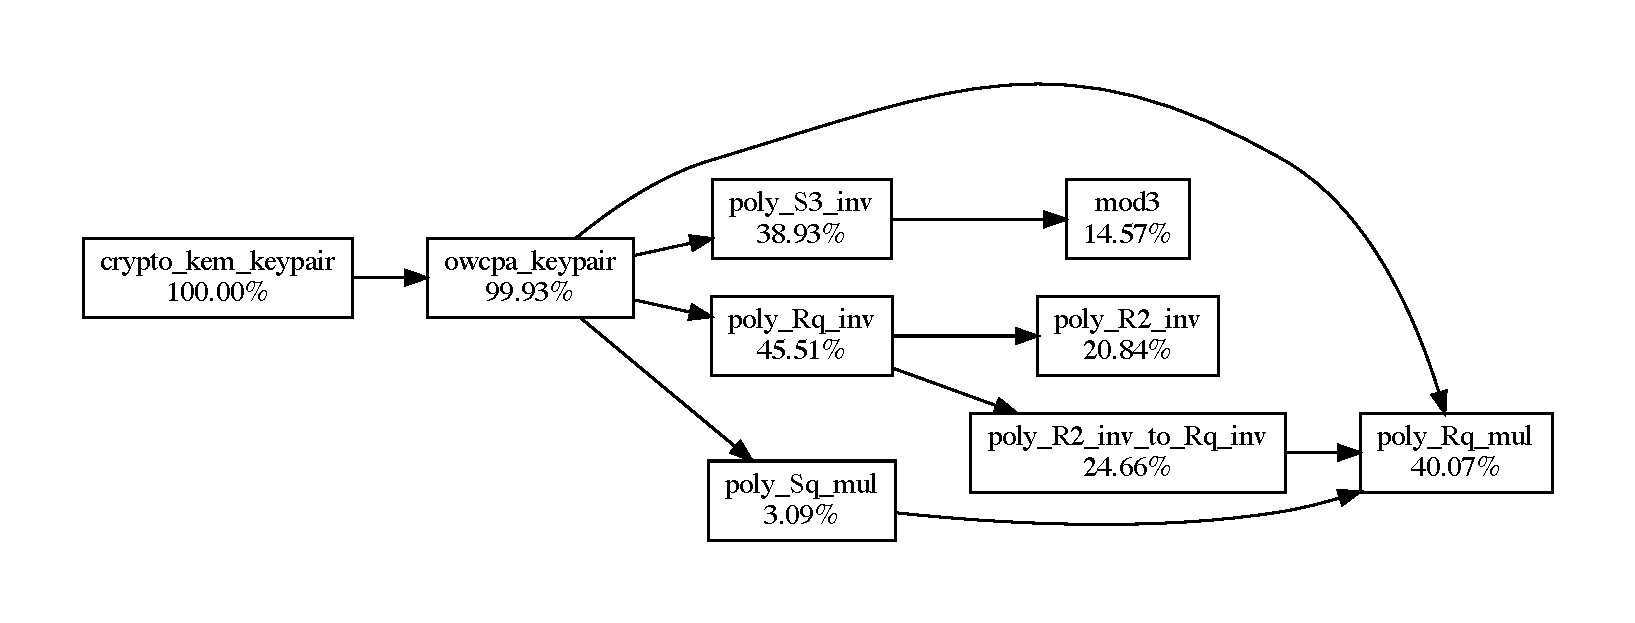
\includegraphics[scale=0.5]{chapters/results/hot-paths/ntru/crypto_kem_keypair.pdf}
    \caption{Relative instruction count of \gls{ntru}'s \textit{crypto\_kem\_keypair}}
    \label{figure:result:hot-paths:ntru:crypto_kem_keypair}
\end{figure}

Figure \ref{figure:result:hot-paths:ntru:crypto_kem_enc} describes the encapsulation API function. The key is generated using random bytes which are fed through 256-bit \gls{aes} in its Electronic Code Book (ECB) configuration to produce uniformly random bytes. Again, we see a significant percentage of the instructions spent in the polynomial library - in \textit{poly\_Rq\_mul}.

\begin{figure}[H]
    \centering
    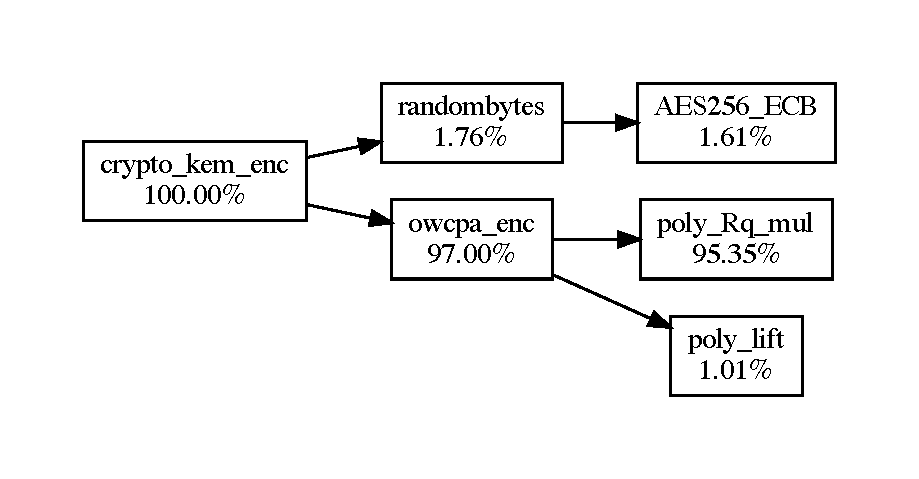
\includegraphics[scale=0.5]{chapters/results/hot-paths/ntru/crypto_kem_enc.pdf}
    \caption{Relative instruction count of \gls{ntru}'s \textit{crypto\_kem\_keypair}}
    \label{figure:result:hot-paths:ntru:crypto_kem_enc}
\end{figure}

The decryption function of \gls{ntru} is presented in figure \ref{figure:result:hot-paths:ntru:crypto_kem_dec}. Virtually all of the instructions spent decrypting (decapsulating) a key is spent in the \textit{poly\_Rq\_mul} function.

\begin{figure}[H]
    \centering
    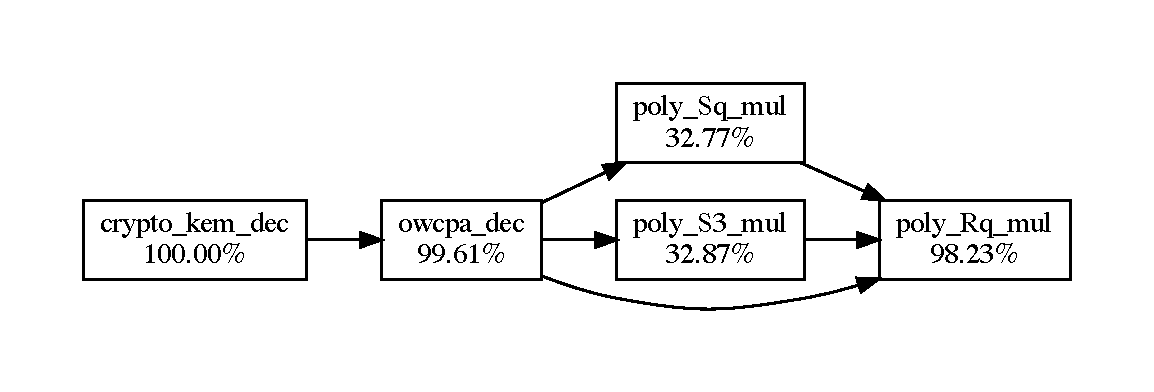
\includegraphics[scale=0.5]{chapters/results/hot-paths/ntru/crypto_kem_dec.pdf}
    \caption{Relative instruction count of \gls{ntru}'s \textit{crypto\_kem\_dec}}
    \label{figure:result:hot-paths:ntru:crypto_kem_dec}
\end{figure}

Looking at the code of \textit{poly\_Rq\_mul} as shown in figure \ref{figure:result:hot-paths:ntru:poly_Rq_mul}, it is evident that the vast majority of instructions are spent on multiplying and adding numbers in loops. The value of \textit{NTRU\_N} corresponds to the parameter set. For \gls{ntru} HRSS 701, the value is 701 and for \gls{ntru} HPS 4096821 the value is 821.

\begin{figure}[H]
    \centering
    \begin{lstlisting}[language=C]
void poly_Rq_mul(poly *r, const poly *a, const poly *b) {
  int k, i;

  for (k = 0; k < NTRU_N; k++) {
    r->coeffs[k] = 0;
    for (i = 1; i < NTRU_N - k; i++) // 10.21%
      r->coeffs[k] += a->coeffs[k + i] * b->coeffs[NTRU_N - i]; // 42.75%
    for (i = 0; i < k + 1; i++) // 8.20%
      r->coeffs[k] += a->coeffs[k - i] * b->coeffs[i]; // 38.79%
  }
}
    \end{lstlisting}
    \caption{Annotated source code of \gls{ntru}'s \textit{poly\_Rq\_mul}}
    \label{figure:result:hot-paths:ntru:poly_Rq_mul}
\end{figure}

To summarize, it is shown that factors such as the speed of \gls{aes} has little to do with the overall performance of the algorithm. Furthermore, it seems as if the polynomial library functions account for the vast majority of instructions spent on key-pair generation, encryption and decryption. The function \textit{poly\_Rq\_mul}, which multiplies two polynomials in $\mathbb{R}^q$, accounts for most of the calculations performed.

\subsection{Classic McEliece}
The \gls{mceliece} reference implementation consists of three API methods - \textit{crypto\_kem\_keypair}, \textit{crypto\_kem\_enc} and \textit{crypto\_kem\_dec} for key-pair generation, encryption (encapsulation) and decryption (decapsulation), respectively\todo{A bit CTRL+C CTRL+V from previous, rewrite?}. These API functions may in turn call several internal functions. We will only present the hot-paths for the \gls{mceliece} 8192128 non-f variant because it can quite accurately represent the hot-paths for all \gls{mceliece} variants.

In figure \ref{figure:result:hot-paths:classic-mceliece:crypto_kem_keypair}, we can see the \textit{crypto\_kem\_keypair} function and its only significant internal function, the \textit{pk\_gen} function that takes up 98.57\% of the execution time. In figure \ref{figure:result:hot-paths:classic-mceliece:pk_gen}, a more in-depth representation of the \textit{pk\_gen} function is presented. In that figure, all of its internal functions are shown. As can be seen, they do not make up much of the accumulated instruction counts. Most of the instructions are inside of the \textit{pk\_gen} function itself.

\begin{figure}[H]
    \centering
    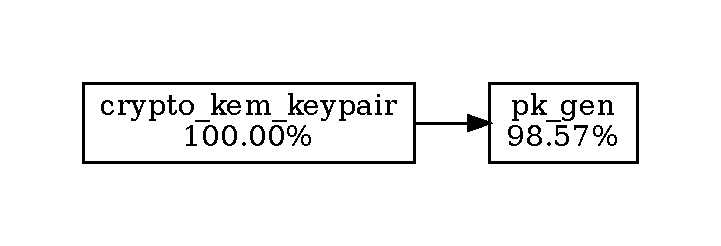
\includegraphics[scale=0.5]{chapters/results/hot-paths/classic-mceliece/8192128/crypto_kem_keypair.pdf}
    \caption{Relative instruction count of \gls{mceliece}'s \textit{crypto\_kem\_keypair}}
    \label{figure:result:hot-paths:classic-mceliece:crypto_kem_keypair}
\end{figure}

\begin{figure}[H]
    \centering
    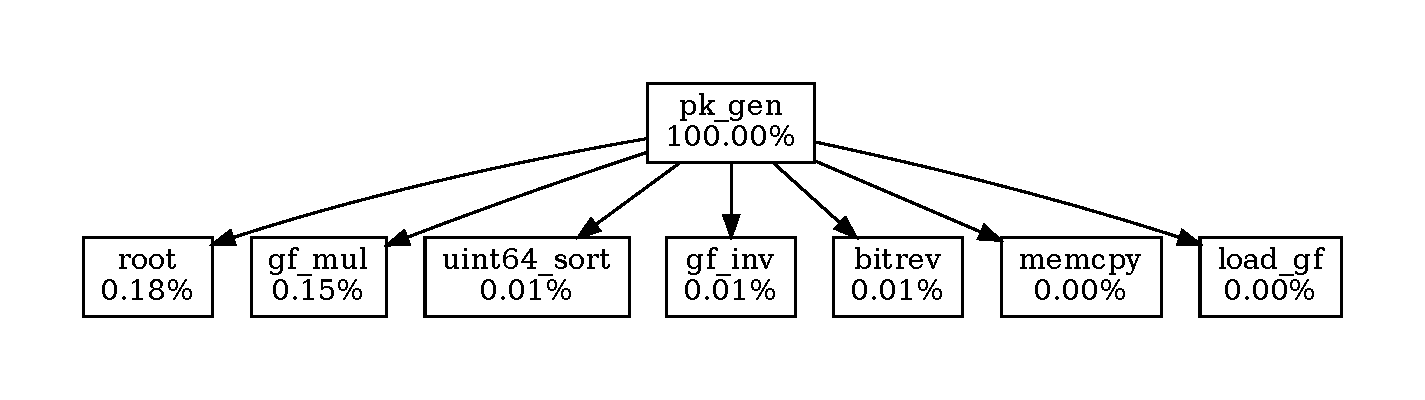
\includegraphics[scale=0.5]{chapters/results/hot-paths/classic-mceliece/8192128/pk_gen.pdf}
    \caption{Relative instruction count of \gls{mceliece}'s \textit{pk\_gen}}
    \label{figure:result:hot-paths:classic-mceliece:pk_gen}
\end{figure}

The encryption function of \gls{mceliece} is presented in figure \ref{figure:result:hot-paths:classic-mceliece:crypto_kem_enc}. Most time is spent in the syndrome function. In figure \ref{figure:result:hot-paths:classic-mceliece:crypto_kem_enc} the decryption function is presented. The majority of the time is spent in the \textit{synd} function.

\begin{figure}[H]
    \centering
    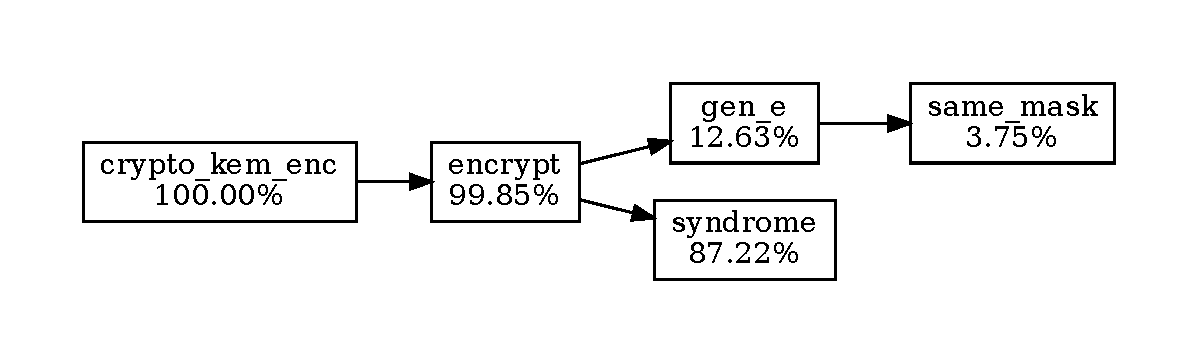
\includegraphics[scale=0.5]{chapters/results/hot-paths/classic-mceliece/8192128/crypto_kem_enc.pdf}
    \caption{Relative instruction count of \gls{mceliece}'s \textit{crypto\_kem\_enc}}
    \label{figure:result:hot-paths:classic-mceliece:crypto_kem_enc}
\end{figure}


\begin{figure}[H]
    \centering
    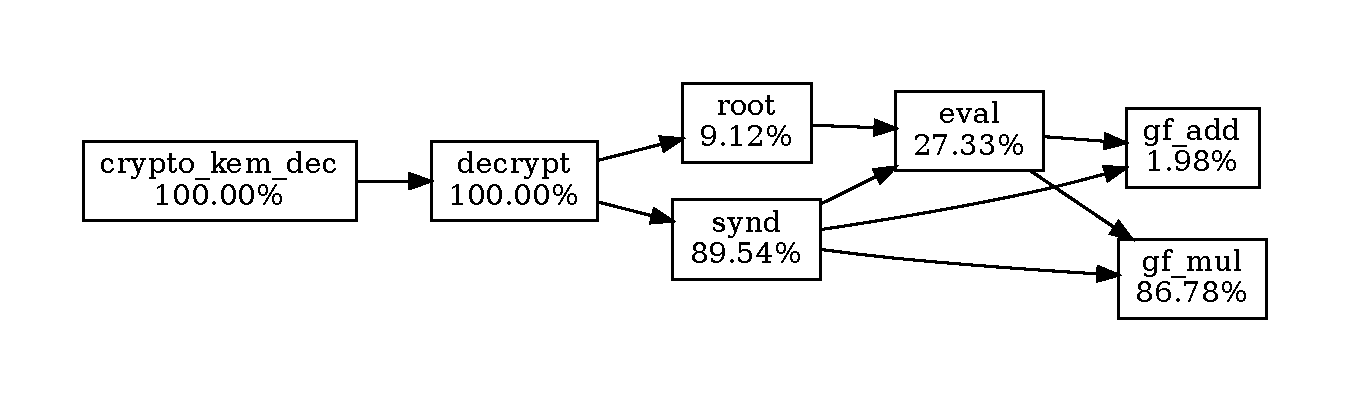
\includegraphics[scale=0.5]{chapters/results/hot-paths/classic-mceliece/8192128/crypto_kem_dec.pdf}
    \caption{Relative instruction count of \gls{mceliece}'s \textit{crypto\_kem\_dec}}
    \label{figure:result:hot-paths:classic-mceliece:crypto_kem_dec}
\end{figure}

\todo[inline]{Var tydliga med hot paths och tid. Exempelvis så lär diagrammet för pk\_gen visa 0\% för vissa funktioner så som root, men om vi ser till hot paths så lär vi se att de kallas flera miljoner gånger. Kanske ha en graf som visar antalet invocations?}

\todo[inline]{Ingen microbenchmark för eval, gf\_mul och gf\_add - de körs så många gånger att overheaden för profiling blev 1000x. McEliece kallar på många många tusen funktioner (hundra tusen, uppemot miljoner?) - det i sig bör ge mer overhead. }

\section{The Performance of Post-Quantum Key Exchange Mechanisms}

This section presents the results of the experiment as outlined in section \ref{section:method:experiment}. It further discusses the performance of \gls{post-quantum} \glspl{kem} and how they may differ on various architectures and hardware.

\subsection{Heap Usage}

As outlined in the method, section \ref{section:method:experiment:phase1:measurements}, we measured the heap usage of the algorithms by monitoring heap allocation and deallocation methods such as malloc using heaptrack. We found that the heap allocation did not change across environments nor between the analyzed optimizations except for some few. As for the implementations, this is rather unsurprising as changing how the allocations worked would alter the behavior of the code. As we found that the heap behavior of the algorithms were consistent throughout our test, we will for the rest of this section not refer to any specific environment or optimization used for the algorithms unless otherwise noted. When talking about allocation, we will refer to the peak allocation - that is, the maximum allocated bytes recorded during a function's lifetime. Our measurements did not capture the peak heap allocation during a benchmark as it would include memory allocations introduced by our tooling. The heap usage metrics do not reflect total memory usage as memory in the form of parameters passed to the algorithms or memory that's part of the stack is not included.

At one point, the \gls{ntru} implementations allocated $264$ bytes generating a keypair. These bytes were allocated by OpenSSL to initialize the library's envelope suite of functions. In context, this is done as the \gls{ntru} implementation uses OpenSSL's \gls{aes} ECB implementation to generate uniform pseduo-random bytes. The invocation of the \gls{aes} function itself resulted in $208$ bytes being allocated by the OpenSSL \gls{aes} ECB implementation. Beyond these bytes, the \gls{ntru} implementation did not require any additional heap allocation during its runtime.

Just like the \gls{ntru} implementations, the \gls{mceliece} implementations make use of OpenSSL to create uniform pseudo-random bytes. As such, the same $264$ bytes are allocated to initialize OpenSSL's envelope suite of functions, as well as the $208$ bytes to actually encrypt random data to produce a uniformly distributed series of bytes. No further allocations were found to be made.

The \gls{ecdhe} and \gls{dhe} implementations are based entirely on functions made available via the OpenSSL library. All of the implementations had an increase in the number of allocations made when compared to \gls{ntru} and \gls{mceliece}. The \gls{dhe} implementation when run in the IBM Community Cloud environment saw an allocation of $16960$ bytes during keypair generation made from a function to calculate the constant-time modulo exponentiation on an arbitrary large number. All other environments allocated $9024$ bytes for the same invocation. Furthermore, the keypair generation saw the allocation of a further $1024$ bytes in the IBM Community Cloud environment seemingly related to the same modulo operation.
The operation of dividing an integer was found to correlate to an additional $536$ bytes in the Cloud Provider 1 environment and $528$ bytes in all of the other environments. The environments saw an additional $1432$ bytes corresponding to the handling of arbitrary large numbers whilst generating a keypair. Fetching random data raised the allocation with $632$ bytes in all environments. There were further allocations made, all of which are summarized in Table \ref{table:results:memory:dhe-heap}. In the table, the peak heap usage of each function of the implementation has been summed up to produce a sum of peaks. This value does not correspond to the peak heap usage of the algorithm as a whole. The \gls{ecdhe} implementation behaved much like the \gls{dhe}, with the peaks differing between some environments. The implementation too worked with OpenSSL's arbitrary numbers and as such had several of the same allocations as the \gls{dhe} implementations. The peaks are presented in Table \ref{table:results:memory:ecdhe-heap}.

\begin{table}
    \centering
    \small
    \caption{Heap Allocation in Bytes for \gls{dhe}}
    \label{table:results:memory:dhe-heap}
    \begin{tabularx}{\linewidth}{X c c c}
        \toprule
        \thead{Environment} & \thead{OpenSSL Version} & \multicolumn{2}{c}{\thead{Sum of Peaks}}\\
        & & \thead{Keypair} & \thead{Exchange} \\
        \midrule
        IBM Community Cloud & 1.1.1g FIPS & 42800 & 39908 \\
        Cloud Provider 1 & 1.1.1 & 14156 & 11934 \\
        Cloud Provider 2 & 1.1.1f & 14040 & 11762\\
        Modern Workstation & 1.1.1f & 14040 & 11762 \\
        Modern Laptop & 1.1.1f & 14040 & 11762 \\
        Old Mid-Range Laptop & 1.1.1f & 14040 & 11762\\
        Old Low-Range Laptop & 1.1.1f & 14040 & 11762\\
        \bottomrule
    \end{tabularx}
\end{table}
\todo{Does not correctly reflect the actual usage? Zero is most likely wrong as the exchange function creates a key. Furthermore, the values currently reflect crypto\_kem\_keypair and crypto\_kem\_exchange, not perform\_keypair and perform\_exchange}

\begin{table}
    \centering
    \small
    \caption{Heap Allocation in Bytes for \gls{ecdhe}}
    \label{table:results:memory:ecdhe-heap}
    \begin{tabularx}{\linewidth}{X c c c c}
        \toprule
        \thead{Environment} & \thead{Curve} & \thead{OpenSSL Version} & \multicolumn{2}{c}{\thead{Sum of Peaks}}\\
        & & & \thead{Keypair} & \thead{Exchange} \\
        \midrule
        IBM Community Cloud & P-256 & 1.1.1g FIPS & 12184 & 0 \\
        IBM Community Cloud & 25519 & 1.1.1g FIPS & 4524 & 1024 \\

        Cloud Provider 1 & P-256 & 1.1.1 & 9220 & 0 \\
        Cloud Provider 1 & 25519 & 1.1.1 & 8380 & 0 \\

        Cloud Provider 2 & P-256 & 1.1.1f & 4884 & 1872 \\
        Cloud Provider 2 & 25519 & 1.1.1f & 2556 & 512\\

        Modern Workstation & P-256 & 1.1.1f & 4884 & 1872 \\
        Modern Workstation & 25519 & 1.1.1f & 2556 & 512 \\
        
        Modern Laptop & P-256 & 1.1.1f & 4884 & 1872 \\
        Modern Laptop & 25519 & 1.1.1f & 2556 & 512 \\
        
        Old Mid-Range Laptop & P-256 & 1.1.1f & 4884 & 1872\\
        Old Mid-Range Laptop & 25519 & 1.1.1f & 2556 & 512\\
        
        Old Low-Range Laptop & P-256 & 1.1.1f & 4884 & 1872\\
        Old Low-Range Laptop & 25519 & 1.1.1f & 2556 & 512\\
        \bottomrule
    \end{tabularx}
\end{table}
\todo[inline]{Does not correctly reflect the actual usage? Zero is most likely wrong as the exchange function creates a key. Furthermore, the values currently reflect crypto\_kem\_keypair and crypto\_kem\_exchange, not perform\_keypair and perform\_exchange

Is this all due to OpenSSL allocating and handling its own memory? Easy to blame them...
}

\subsection{Stack Usage}

In terms of stack usage, the results vary between the implementations, compilers and features. For instance, the polynomial math function poly\_Rq\_mul in \gls{ntru}, which was identified as constituting most of the time spent in the algorithm, varies between taking up $70499$ and $188$ bytes. In all environments, the HPS 4096821 AVX2 variant takes up $70499$ bytes. This does not change between compilers or optimization flags, which could be due to the fact that the implementation is written in assembly - leaving little room for the compiler to alter the behavior. The same goes for the HRSS 701 variant of \gls{ntru} - the size is consistently 55317 bytes across environments and optimization flags. The lowest sizes are found when the reference implementation is compiled with optimization. The sizes are presented in Table \ref{table:results:memory:ntru-stack}. Although the optimization flags used were not chosen for improving the size of the binary, the size of the function has been lowered in all cases. Although the same version of GCC was used for several environments, the results differed between $188$ and $192$ bytes. Clang continually produced larger regions than GCC. Furthermore, more recent versions of the compilers seem to have produced smaller sizes.

\begin{table}
    \small
    \centering
    \caption{Stack Size of poly\_Rq\_mul in Bytes for the Optimized Reference Implementation}
    \label{table:results:memory:ntru-stack}
    \begin{tabularx}{\linewidth}{X c c c c}
        \toprule
        \thead{Environment} & \thead{Compiler} & \thead{Compiler Version} & \thead{Optimized Size} & \thead{Reference Size}\\
        \midrule
        Cloud Provider 1 & clang & 6.0.0 & 702 & - \\
        IBM Community Cloud & clang & 10.0.1 & 522 & - \\
        Cloud Provider 2 & clang & 10.0.0 & 380 & - \\
        Modern Laptop & clang & 10.0.0 & 380 & - \\
        Modern Workstation & clang & 10.0.0 & 380 & - \\
        Modern Laptop & clang & 10.0.0 & 380 & - \\
        Old Low-Range Laptop & clang & 10.0.0 & 300 & - \\
        Old Mid-Range Laptop & clang & 10.0.0 & 300 & - \\
    
        IBM Community Cloud & gcc & 8.3.1 & 242 & 382 \\
        Old Low-Range Laptop & gcc & 9.3.0 & 196 & 255 \\
        Old Mid-Range Laptop & gcc & 9.3.0 & 196 & 255 \\
        Cloud Provider 1 & gcc & 7.5.0 & 192 & 253\\
        Cloud Provider 2 & gcc & 9.3.0 & 188 & 255\\
        Modern Laptop & gcc & 9.3.0 & 188 & 255\\
        Modern Workstation & gcc & 9.3.0 & 188 & 255\\
        \bottomrule
    \end{tabularx}
\end{table}

The same correlation between optimization flags and compiler versions could not be found in the case of \gls{mceliece} and pk\_gen. In that case, the largest recorded size was found in IBM Community Cloud's optimized reference implementation with $22858$ bytes. The optimized AVX2 implementation of the Modern Workstation and Modern Laptop came second with $22123$ bytes. Lastly, the smallest size recorded was found in the optimized reference implementation of Old Mid-Range Laptop and Old Low-Range Laptop at $2026$ bytes.

As for other functions of the \glspl{kem}, the data is too massive to comprehensively refer to here. There are, however, tables in the appendix for average sizes as compared to the reference implementation compiled with GCC. In Table \ref{table:result:ntru-average-stack-increase-cloud}, for example, one may see that Clang seems to produce smaller binaries. Furthermore, the optimized AVX2 builds result in the largest binaries - with symbols taking 8-10 times the size of the reference implementation.

\todo[inline]{Discuss stack usage of ECDHE, DHE?}

\subsection{Parameter Sizes}

The measurements presented up until this point have been related to either the runtime behavior of the algorithms, or the static requirements they place on the environment in the form of stack usage. These measurements have not included the parameters fed to the algorithms - which could affect real-world applications. The remaining part of this section will present data gathered from the various implementations.

The \glspl{kem} tested conform to the same API. Their signatures are presented in figure \ref{figure:result:memory:kem-api}. The function crypto\_kem\_keypair, which generates a keypair takes in a public key and a secret key. The encapsulation function, crypto\_kem\_enc, takes in a ciphertext buffer, a key buffer and the public key of a peer. Lastly, the decapsulation function, crypto\_kem\_dec takes in a key buffer, the ciphertext as received from a peer and the secret key. The sizes of these parameters differ between algorithms and implementations - but is not changed depending on the environment or optimizations. Table \ref{table:results:memory:kem-parameter-sizes} shows the sizes of the parameters in bytes. The sizes do not differ between the semi-systematic (f) variants of \gls{mceliece}. Therefore only two variants of \gls{mceliece} are presented.

\begin{figure}
    \centering
    \begin{lstlisting}[language=C]
int crypto_kem_keypair(unsigned char *public_key, unsigned char *private_key);
int crypto_kem_enc(unsigned char *ciphertext, unsigned char *key, const unsigned char *public_key);
int crypto_kem_dec(unsigned char *key, const unsigned char *ciphertext, const unsigned char *private_key);
    \end{lstlisting}
    \caption{The API of the \gls{kem} Implementations}
    \label{figure:result:memory:kem-api}
\end{figure}

\begin{table}
    \centering
    \small
    \caption{Parameter Sizes in Bytes of the \glspl{kem} Under Test}
    \label{table:results:memory:kem-parameter-sizes}
    \begin{tabularx}{\linewidth}{X c c c c c}
        \toprule
        \thead{Algorithm} & \thead{Parameters} & \thead{public\_key} & \thead{private\_key} & \thead{ciphertext} & \thead{key}\\
        \midrule
        \gls{mceliece} & 8192128(f) & 1357824 & 14120 & 240 & 32 \\
        \gls{mceliece} & 6960119(f) & 1047319 & 13948 & 226 & 32 \\
        \gls{ntru} & HRSS 701 & 1138 & 1450 & 1138 & 32 \\
        \gls{ntru} & HPS 4096821 & 1230 & 1590 & 1230 & 32 \\
        \bottomrule
    \end{tabularx}
\end{table}

The APIs are similar, but not the same for the \gls{kex} implementations. That is due to \gls{dh} requiring the so called Diffie-Hellman Parameters $p$ and $g$. The APIs are shown in figure \ref{figure:results:memory:kex-api}. As with the \gls{kem} implementations, the \gls{kex} implementations use two buffers for a public and a private key when generating a keypair. The \gls{dh} implementation also requires the previously mentioned domain parameters $p$ and $g$ - both buffers of bytes containing the respective parameter. The crypto\_dh\_enc functions further use a key buffer. There is no analogous ciphertext as the \glspl{kex} are fundamentally different from the \glspl{kem} as covered in \ref{section:background:diffie-hellman}. The sizes of the parameters are presented in Table \ref{table:results:memory:kex-parameter-sizes}.

\begin{figure}
    \centering
    \begin{lstlisting}[language=C]
// Diffie-Hellman
int crypto_dh_keypair(unsigned char *public_key, unsigned char *private_key, unsigned char *p, unsigned char *g);

// Diffie-Hellman
int crypto_dh_enc(unsigned char *key, const unsigned char *private_key, const unsigned char *public_key, unsigned char *p, unsigned char *g);

// Elliptic-Curve Diffie-Hellman
int crypto_dh_keypair(unsigned char *public_key, unsigned char *private_key);

// Elliptic-Curve Diffie-Hellman
int crypto_dh_enc(unsigned char *key, const unsigned char *private_key, const unsigned char *public_key);
    \end{lstlisting}
    \caption{The API of the \gls{kex} Implementations}
    \label{figure:results:memory:kex-api}
\end{figure}

\begin{table}
    \centering
    \small
    \caption{Parameter Sizes in Bytes of the \glspl{kex} Under Test}
    \label{table:results:memory:kex-parameter-sizes}
    \begin{tabularx}{\linewidth}{X c c c c c c}
        \toprule
        \thead{Algorithm} & \thead{Parameters} & \thead{public\_key} & \thead{private\_key} & \thead{$p$} & \thead{$g$} & \thead{key}\\
        \midrule
        \gls{dh} & 2048    &255 & 255 & 256  & 1 & 32 \\
        \gls{ecdh} & P-256 & 65 & 32 & - & - & 32 \\
        \gls{ecdh} & 25519 & 32 & 32 & - & - & 32 \\
        \bottomrule
    \end{tabularx}
\end{table}

\subsection{Sequential Performance}

The performance of the algorithms in a single run was analyzed by performing a thousand sequential runs in series, for each algorithm under test at two different occasions. The complete method is outlined in section \ref{section:method:experiment:phase1}.

As covered in section \ref{section:background:mceliece}, \gls{mceliece} supports two forms of keypair-generation algorithms - a systematic form and a semi-systematic form. The systematic forms, such as \gls{mceliece} 8192128 and the semi-systematic forms, such as \gls{mceliece} 8192128f, use different algorithms for generating the keypairs. The authors of the \gls{nist} submission state that these two forms may have different performance characteristics \cite{mceliece2020}. In Table \ref{table:results:sequential-mceliece-6960119-keypair-modern-workstation}, these two forms can be seen with every set of performance improvements tested in the experiment. As can be seen in the table, the reference implementation in its systematic form is remarkably inconsistent, with a standard deviation of $20580.20$ as compared to the $6.91$ of the semi-systematic form. The change in performance characteristics is also visible in the mean, with the semi-systematic form taking about $30\%$ of the time on average as compared to the systematic form. In both cases, the \gls{avx2} implementation has the second largest standard deviation with $302.58$ and $6.91$ for the systematic form and the semi-systematic form, respectively. Despite being a \gls{simd} implementation, \gls{avx2} performs worse than the optimized reference implementation in both forms of the algorithm. The optimized \gls{avx2} implementation, however, outperforms the optimized reference implementation with four to six times the performance. The same results were found to generalize for several environments, as shown in Table \ref{table:results:sequential:mceliece-6960119-keypair} and \ref{table:results:sequential:mceliece-6960119f-keypair}.

\begin{table}
    \centering
    \caption{Duration of \gls{mceliece} 6960119 Keypair Generation On Modern Workstation}
    \label{table:results:sequential-mceliece-6960119-keypair-modern-workstation}
    \begin{tabularx}{\linewidth}{l X c c c c}
        \toprule
        \thead{Compiler} & \thead{Flags} & \thead{Mean} & \thead{Standard\\Deviation} & \multicolumn{2}{c}{\thead{95\% CI}}\\
        & & & & \thead{Lower} & \thead{Upper} \\
        \midrule
        \thead{non-systematic form}\\
                         gcc &                  ref &             21885.78 &             20580.20 &             17376.37 &             26395.19\\
                         gcc &                 avx2 &               562.39 &               302.58 &               549.13 &               575.66\\
                       clang &        ref-optimized &               696.65 &               571.35 &               671.60 &               721.70\\
                         gcc &        ref-optimized &               421.15 &               317.77 &               407.22 &               435.09\\
                         gcc &       avx2-optimized &                72.26 &                38.78 &                70.56 &                73.96\\
                       clang &       avx2-optimized &                70.28 &                38.12 &                68.61 &                71.95\\
    
    \midrule
      \thead{semi-systematic form}\\
                        gcc &                  ref &              6476.15 &                 6.91 &              6475.33 &              6476.97\\
                         gcc &                 avx2 &               315.24 &                 0.96 &               315.19 &               315.28\\
                       clang &        ref-optimized &               230.14 &                 0.74 &               230.11 &               230.18\\
                         gcc &        ref-optimized &               159.12 &                 0.61 &               159.09 &               159.15\\
                         gcc &       avx2-optimized &                40.45 &                 0.84 &                40.42 &                40.49\\
                       clang &       avx2-optimized &                39.93 &                 1.50 &                39.86 &                39.99\\
        \bottomrule
    \end{tabularx}
\end{table}

In all environments but one, we found consistent performance throughout all sequential runs, non-deterministic behavior and outliers aside. The Cloud Provider 2 environment provided inconsistent results throughout the sequential performance benchmarks - across various algorithms and runs. As seen in figure \ref{figure:results:sequential:mceliece-decrpyt-cloud-provider-2}, there are several occasions where the performance shift over time. In the figure, the speedup relative to the reference GCC implementation is used as opposed to the absolute duration of each iteration. Depending on how deterministic the behavior of the algorithms are, as well as how stable the environment is, one could have expected more or less the same performance throughout the test. As the Cloud Provider 2 environment uses two virtual CPU cores, it is not entirely unexpected to find such inconsistent results. The same behavior was not found in any of the environments tested with dedicated hardware, nor the Cloud Provider 1 environment.

\begin{figure}
    \centering
    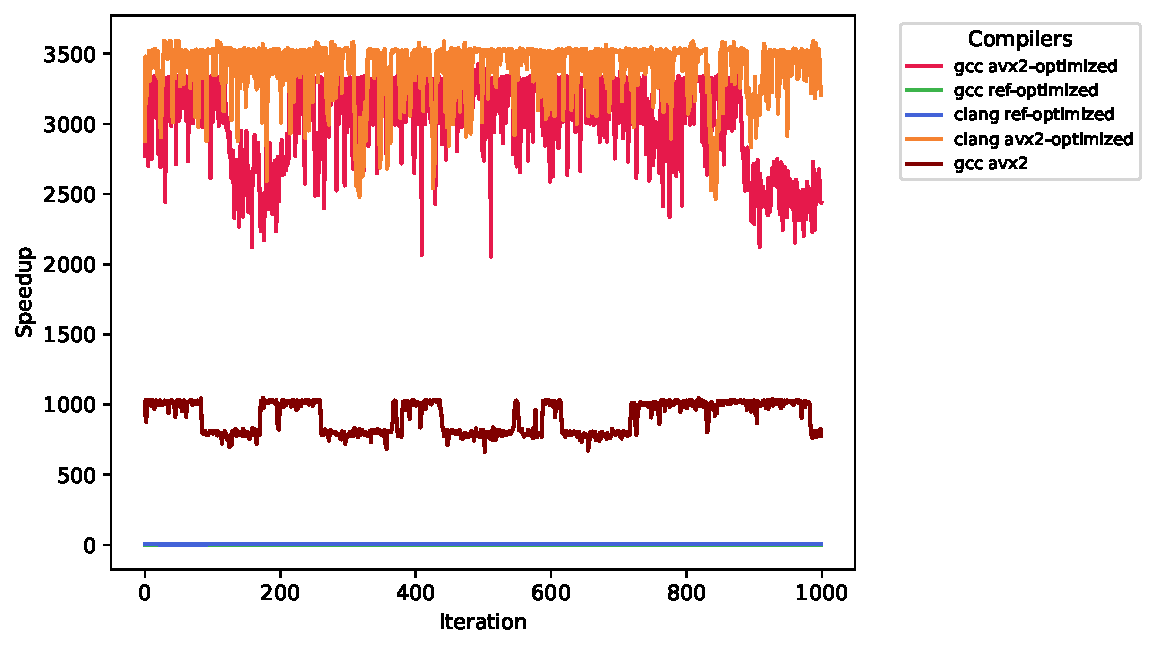
\includegraphics[scale=0.75]{chapters/results/sequential/mceliece_6960119_decrypt_Cloud Provider 2.pdf}
    \caption{The Speedup of \gls{mceliece} 6960119 Over Time. Note that the green and blue lines are coincident}
    \label{figure:results:sequential:mceliece-decrpyt-cloud-provider-2}
\end{figure}

In Table \ref{figure:results:sequential:ntru-hrss701} all of the average durations and speedups for each optimization and environment are shown. In the table, one may see conclusive evidence that the optimized \gls{avx2} implementations perform the best in all environments with support for \gls{avx2}. It is not clear, however, what compiler produces the best performance. In the environments without support for \gls{avx2}, the optimized reference implementation performed the best. Just as with the \gls{avx2} implementations, it's unclear whether or not GCC or Clang produced the best results. It seems as if GCC produces more consistent results, with less variation in the averages. In the Old Low-Range Laptop environment, for example, one may see that Clang requires about two times the duration of the comparable subject compiled with GCC. In other cases, Clang seems to be on par with, or better than, GCC. As the speedup is percentual based on the environment, one may expect them to be similar across environments. That is, the speedup of using \gls{avx2} instead of the reference implementation, should in theory be similar on both the Modern Workstation and Modern Laptop, for example. In practice we found this to not be true. Although similar, the \gls{avx2} implementation compiled and optimized by Clang on the Modern Workstation has an additional 78 times speedup when compared to the Modern Laptop. On the other hand, the Old Mid-Range Laptop and the Old Low-Range Laptop perform near identically in terms of speedup.

\begin{table}[H]
    \centering
    \footnotesize
    \caption{Sequential Duration and Speedup of \gls{ntru} HRSS 701}
    \label{figure:results:sequential:ntru-hrss701}
    \begin{tabularx}{\linewidth}{l l c c c c c c}
        \toprule
        \thead{Environment} & \thead{Flags} & \multicolumn{3}{c}{\thead{Average Duration (ms)}} & \multicolumn{3}{c}{\thead{Speedup}}\\
        & & keypair & encrypt & decrypt & keypair & encrypt & decrypt \\
        \midrule
        \multirowcell{8}{Modern\\ Workstation}
          & \textbf{gcc} & & & & & \\
          & ref & 34.373 & 0.910 & 2.660 & 0.0 & 0.0 & 0.0\\
          & ref-optimized & 3.386 & 0.235 & 0.641 & 9.2 & 2.9 & 3.2\\
          & avx2 & 0.240 & 0.029 & 0.037 & 142.2 & 30.8 & 71.1\\
          & avx2-optimized & 0.066 & 0.018 & 0.016 & 517.4 & 49.7 & 167.3\\
          & \textbf{clang} & & & & & \\
          & ref-optimized & 5.786 & 0.206 & 0.563 & 4.9 & 3.4 & 3.7\\
          & avx2-optimized & 0.070 & 0.016 & 0.015 & 491.8 & 54.3 & 181.2\\
          \midrule
          \multirowcell{8}{Modern\\ Laptop}
          & \textbf{gcc} & & & & & \\
          & ref & 41.808 & 1.149 & 3.321 & 0.0 & 0.0 & 0.0\\
          & ref-optimized & 4.202 & 0.278 & 0.816 & 8.9 & 3.1 & 3.1\\
          & avx2 & 0.322 & 0.051 & 0.048 & 128.9 & 21.5 & 67.7\\
          & avx2-optimized & 0.085 & 0.026 & 0.024 & 491.4 & 42.5 & 138.3\\
          & \textbf{clang} & & & & & \\
          & ref-optimized & 7.250 & 0.264 & 0.772 & 4.8 & 3.4 & 3.3\\
          & avx2-optimized & 0.087 & 0.024 & 0.032 & 479.0 & 46.1 & 103.1\\
          \midrule
          \multirowcell{5}{Old\\ Mid-Range\\ Laptop}
          & \textbf{gcc} & & & & & \\
          & ref & 61.040 & 1.579 & 4.584 & 0.0 & 0.0 & 0.0\\
          & ref-optimized & 6.376 & 0.416 & 1.131 & 8.6 & 2.8 & 3.1\\
          & \textbf{clang} & & & & & \\
          & ref-optimized & 12.342 & 0.483 & 1.305 & 3.9 & 2.3 & 2.5\\
          \midrule
          \multirowcell{5}{Old\\ Low-Range\\ Laptop}
          & \textbf{gcc} & & & & & \\
          & ref & 77.043 & 1.952 & 5.667 & 0.0 & 0.0 & 0.0\\
          & ref-optimized & 7.929 & 0.502 & 1.391 & 8.7 & 2.9 & 3.1\\
          & \textbf{clang} & & & & & \\
          & ref-optimized & 15.615 & 0.600 & 1.670 & 3.9 & 2.3 & 2.4\\
          \midrule
          \multirowcell{8}{Cloud\\ Provider\\ 1}
          & \textbf{gcc} & & & & & \\
          & ref & 50.464 & 1.353 & 3.959 & 0.0 & 0.0 & 0.0\\
          & ref-optimized & 5.607 & 0.394 & 1.091 & 8.0 & 2.4 & 2.6\\
          & avx2 & 0.408 & 0.056 & 0.065 & 122.7 & 23.3 & 60.2\\
          & avx2-optimized & 0.114 & 0.027 & 0.028 & 442.4 & 49.8 & 142.7\\
          & \textbf{clang} & & & & & \\
          & ref-optimized & 8.137 & 0.286 & 0.797 & 5.2 & 3.7 & 4.0\\
          & avx2-optimized & 0.108 & 0.031 & 0.029 & 465.6 & 43.1 & 134.6\\
          \midrule
          \multirowcell{8}{Cloud\\ Provider\\ 2}
          & \textbf{gcc} & & & & & \\
          & ref & 59.660 & 1.593 & 4.686 & 0.0 & 0.0 & 0.0\\
          & ref-optimized & 5.778 & 0.404 & 1.106 & 9.3 & 2.9 & 3.2\\
          & avx2 & 0.477 & 0.051 & 0.068 & 124.2 & 30.5 & 68.4\\
          & avx2-optimized & 0.148 & 0.057 & 0.054 & 400.9 & 26.9 & 86.4\\
          & \textbf{clang} & & & & & \\
          & ref-optimized & 10.064 & 0.367 & 0.966 & 4.9 & 3.3 & 3.9\\
          & avx2-optimized & 0.130 & 0.037 & 0.030 & 458.8 & 42.3 & 152.6\\
          \midrule
          \multirowcell{5}{IBM\\ Community\\ Cloud}
          & \textbf{gcc} & & & & & \\
          & ref & 63.455 & 2.105 & 6.066 & 0.0 & 0.0 & 0.0\\
          & ref-optimized & 7.202 & 0.485 & 1.426 & 7.8 & 3.3 & 3.3\\
          & \textbf{clang} & & & & & \\
          & ref-optimized & 8.815 & 0.389 & 1.136 & 6.2 & 4.4 & 4.3\\
        \bottomrule
    \end{tabularx}
\end{table}

By studying the average duration taken by the various subjects in each environment, one may clearly see that \gls{avx2} performs the best when it's available. When \gls{avx2} is not available, the optimized reference implementation performs the best. The results are however indecisive in terms of what compiler performed the best in each environment.

\begin{table}[H]
    \centering
    \small
    \caption{Comparison of CPU Cycles of Our and the Submission Authors' Measurements}
    \label{table:results:sequential:nist-vs-ours}
    \begin{tabularx}{\linewidth}{X c r r r r}
        \toprule
        \thead{Algorithm} & \thead{Operation} & \multicolumn{2}{c}{Reference Cycles} & \multicolumn{2}{c}{AVX2 Cycles}\\
        & & \thead{Ours} & \thead{Theirs} & \thead{Ours} & \thead{Theirs}\\
        \midrule
        \multicolumn{4}{l}{\gls{mceliece}}\\
        mceliece6960119 & keypair & 2063786004 & \multicolumn{1}{c}{-} & 380284953 & 438217685\\
        mceliece6960119f & keypair & 801046672 & \multicolumn{1}{c}{-} & 207228427 & 246508730\\
        mceliece8192128 & keypair & 2227969526 & \multicolumn{1}{c}{-} & 453667430 & 514489441\\
        mceliece8192128f & keypair & 835007190 & \multicolumn{1}{c}{-} & 275660079 & 316202817\\
        
        mceliece6960119(f) & encrypt & 41429828 & \multicolumn{1}{c}{-} & 205954 & 161224\\
        mceliece8192128(f) & encrypt & 40992651 & \multicolumn{1}{c}{-} & 238652 & 178093\\
        
        mceliece6960119(f) & decrypt & 41429828 & \multicolumn{1}{c}{-} & 205954 & 301480\\
        mceliece8192128(f) & decrypt & 40992651 & \multicolumn{1}{c}{-} & 238652 & 326531\\
        \midrule
        \multicolumn{4}{l}{\gls{ntru}}\\
        ntruhps4096821 & keypair & 22392736 & 22511180 & 688900 & 431667\\
        ntruhrss701 & keypair & 16893273 & 16487419 & 320425 & 340823\\
        
        ntruhps4096821 & encrypt & 6782969 & 1566922 & 297125 & 98809\\
        ntruhrss701 & encrypt & 4552302 & 1069326 & 88768 & 50441\\
        
        ntruhps4096821 & decrypt & 18128147 & 4237744 & 104332 & 75384\\
        ntruhrss701 & decrypt & 13511286 & 3113303 & 190756 & 62267\\
        \bottomrule
    \end{tabularx}
\end{table}
\todo{Comment on table, mention that it's Modern Workstation}
% mceliece Ours: ref-optimized modern workstation, theirs Intel  Xeon ref -O3 etc...
% ntru: ours ref-optimized modern workstation, theirs intel i 3-6000? etc...
% ntru ours: avx2-optimized modern ... theris i7-4770K (Haswell)
% supercop 1% av ntruhps4096821, 60% av ntruhrss701 wtf?
% amd64; CoffeeLake (906ea); 2017 Intel Core i7-8700; 6 x 3200MHz; bitvise, supercop-20190910
% https://bench.cr.yp.to/results-kem.html
% NTRU stated that their results were to be presented on the same page, but they were not

\subsection{Throughput Performance}

As outlined in section \ref{section:method:experiment:phase2}, the throughput of the algorithms in each environment under test was evaluated for a series of parallelism configurations. The initial plan was to use the best-performing implementation of each algorithm for each environment, as identified by the sequential benchmarks. The results from the sequential benchmark previously presented were not conclusive and we therefore ended up running the parallel benchmarks on both GCC and Clang builds of the best-performing variant.

The throughput of the \gls{dhe} implementation was found to consistently slow down after the number of threads surpass the number of physical cores multiplied with the degree of \gls{smt}. In figure \ref{figure:results:throughput:dh-old-mid-range-laptop}, the throughput of the Old Mid-Range Laptop can be seen. Old Mid-Range Laptop, a dual core machine with four threads, levels off at the four threads mark. As mentioned previously in section \ref{table:method:experiment:phase1:implementation-configurations}, two variants of \gls{dhe} were tested - one compiled and optimized by GCC, the other by Clang - both of which are presented in the aforementioned figure. The performance difference between the two compilers seem to be negligible, which one may expect as the OpenSSL library used to provide the implementation with virtually all of its functionality is dynamically linked. That means that it is not recompiled nor optimized by the compiler used to compile the program. The same leveling found in Old Mid-Range Laptop was also identified in all of the other environments tested.

\begin{figure}
    \centering
    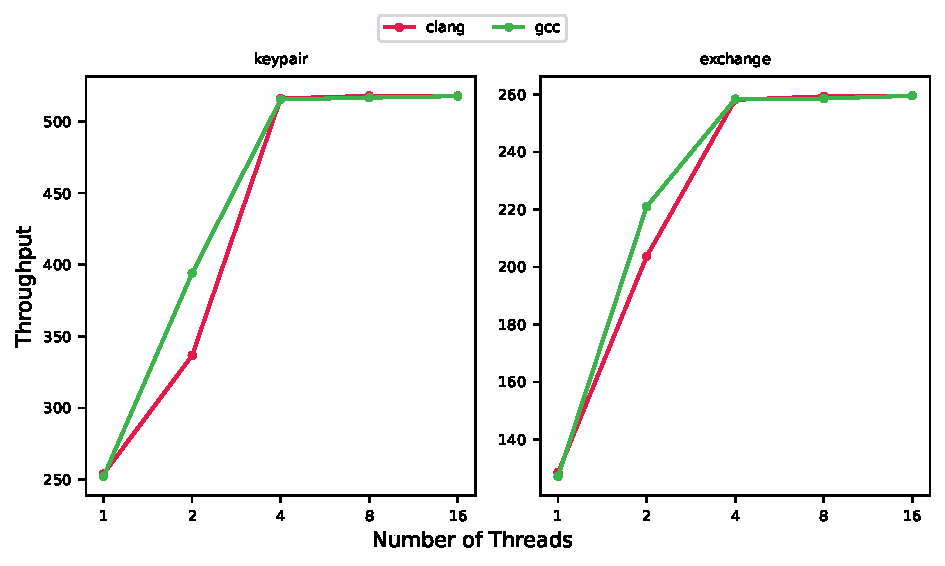
\includegraphics[scale=0.75]{chapters/results/throughput/Old Mid-Range Laptop_dh.pdf}
    \caption{Throughput of \gls{dhe} on Old Mid-Range Laptop for Various Thread Counts}
    \label{figure:results:throughput:dh-old-mid-range-laptop}
\end{figure}

The \gls{ecdhe} implementation was found to be drastically more performant than the \gls{dhe} implementation, with a speedup ranging between 5 to 350 times the throughput. The highest increase in performance was found in the IBM Community Cloud environment, seen in figure \ref{figure:results:throughput:ecdh-ibm-community-cloud}. The throughput, drastically dropped when tested on four or more threads. The peak at two threads coincides with the number of available threads\footnote{It is unknown whether or not the cores are physical cores, logical cores or virtual cores} of the environment. What's more is a 30\% drop in throughput in the exchange phase of the \gls{x25519} implementation compiled and optimized using GCC. The drop was consistent through both of the runs of the complete benchmark at two completely different occasions\todo{analyze further?}. It was found that during the \gls{x25519} run on four threads, two of the threads consistently performed half of the throughput of the other two.

\begin{figure}
    \centering
    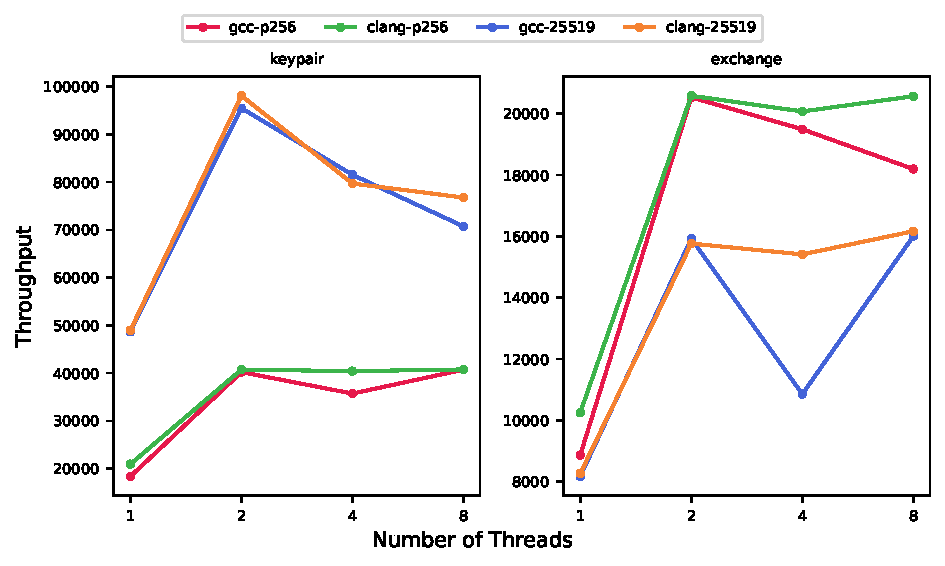
\includegraphics[scale=0.75]{chapters/results/throughput/IBM Community Cloud_ecdh.pdf}
    \caption{Throughput of \gls{ecdhe} on IBM Community Cloud for Various Thread Counts}
    \label{figure:results:throughput:ecdh-ibm-community-cloud}
\end{figure}

In Table \ref{table:results:throughput:ecdh-25519}\todo{explain table}, the throughput for each environment is shown for the \gls{x25519} keypair generation. As can be seen, the IBM Community Cloud environment outperforms all of the other environments when using one or two threads. The mainframe and cloud hardware tested saw a decrease in throughput at one point or another, whilst the consumer hardware continually performed better with more threads for all the thread counts tested\todo{explain table - what optimizations were used, what are the values?}.

    \begin{table}[H]
        \centering
        \small
        \caption{Parallel Throughput Runs for X25519 Keypair Generation}
        \label{table:results:throughput:ecdh-25519}
        \begin{tabularx}{\linewidth}{X c c c c c c c c}
            \toprule
            \thead{Environment} & \thead{Compiler} & \multicolumn{7}{c}{\thead{Threads}}\\
            & & 1 & 2 & 4 & 8 & 16 & 32 & 64 \\
            \midrule
\multirowcell{4}{Cloud\\ Provider\\ 1} & 
\multirow{2}{*}{gcc} & 20066 & 28639 & 41075 & 39385 & 43578\\
 & & 1.0 & 1.43 & 2.05 & 1.96 & 2.17\\
\cmidrule[0.05em](){3-9} & 
\multirow{2}{*}{clang} & 22183 & 28580 & 45468 & 42508 & 45103\\
 & & 1.11 & 1.42 & 2.27 & 2.12 & 2.25\\
            \midrule
\multirowcell{4}{Cloud\\ Provider\\ 2} & 
\multirow{2}{*}{gcc} & 18784 & 35641 & 34956 & 35292\\
 & & 1.0 & 1.90 & 1.86 & 1.88\\
\cmidrule[0.05em](){3-9} & 
\multirow{2}{*}{clang} & 15818 & 35574 & 31504 & 36365\\
 & & 0.84 & 1.89 & 1.68 & 1.94\\
            \midrule
\multirowcell{4}{IBM\\ Community\\ Cloud} & 
\multirow{2}{*}{gcc} & 48666 & 95482 & 81536 & 70727\\
 & & 1.0 & 1.96 & 1.68 & 1.45\\
\cmidrule[0.05em](){3-9} & 
\multirow{2}{*}{clang} & 48960 & 98079 & 79706 & 76773\\
 & & 1.01 & 2.02 & 1.64 & 1.58\\
            \midrule
\multirowcell{4}{Modern\\ Laptop} & 
\multirow{2}{*}{gcc} & 10654 & 22234 & 42188 & 65254 & 68590 & 76830\\
 & & 1.0 & 2.09 & 3.96 & 6.12 & 6.44 & 7.21\\
\cmidrule[0.05em](){3-9} & 
\multirow{2}{*}{clang} & 10605 & 20794 & 41605 & 63372 & 68244 & 77024\\
 & & 1.00 & 1.95 & 3.91 & 5.95 & 6.41 & 7.23\\
            \midrule
\multirowcell{4}{Modern\\ Workstation} & 
\multirow{2}{*}{gcc} & 13458 & 26474 & 51051 & 140658 & 186775 & 204705 & 235189\\
 & & 1.0 & 1.97 & 3.79 & 10.45 & 13.88 & 15.21 & 17.48\\
\cmidrule[0.05em](){3-9} & 
\multirow{2}{*}{clang} & 12728 & 26607 & 51969 & 143312 & 191370 & 205084 & 233812\\
 & & 0.95 & 1.98 & 3.86 & 10.65 & 14.22 & 15.24 & 17.37\\
            \midrule
\multirowcell{4}{Old\\ Low-Range\\ Laptop} & 
\multirow{2}{*}{gcc} & 8880 & 17512 & 24091 & 24448 & 26801\\
 & & 1.0 & 1.97 & 2.71 & 2.75 & 3.02\\
\cmidrule[0.05em](){3-9} & 
\multirow{2}{*}{clang} & 7758 & 19524 & 23932 & 26041 & 26870\\
 & & 0.87 & 2.20 & 2.70 & 2.93 & 3.03\\
            \midrule
\multirowcell{4}{Old\\ Mid-Range\\ Laptop} & 
\multirow{2}{*}{gcc} & 11238 & 20977 & 28151 & 30188 & 31114\\
 & & 1.0 & 1.87 & 2.50 & 2.69 & 2.77\\
\cmidrule[0.05em](){3-9} & 
\multirow{2}{*}{clang} & 10295 & 15511 & 28881 & 30570 & 31859\\
 & & 0.92 & 1.38 & 2.57 & 2.72 & 2.83 \\
            \bottomrule
        \end{tabularx}
    \end{table}
    

When looking at the throughput of \gls{mceliece} in environments which do not support \gls{avx2}, such as the IBM Community Cloud presented in figure \ref{figure:results:throughput:mceliece-ibm-community-cloud}, we found that the keypair and decrypt throughput was significantly lower than that of the encrypt stage. The performance of the decrypt stage was roughly $0.1\%$ of the encrypt stage. Furthermore, the parameter set with the largest parameters - \gls{mceliece} 8192128f achieved a higher encryption throughput than the \gls{mceliece} 6960119f variant\todo{not true! It's the other way around!}. There is also a large difference between the encrypt stage of the subjects compiled and optimized using GCC and those using Clang. Lastly, it seems as if the throughput levels off after the number of used threads surpass the number of available threads. As mentioned, the same overall behavior was found in all of the environments using the optimized reference implementation for benchmarking the parallel throughput, such as Old Mid-Range Laptop in figure \ref{figure:results:throughput:mceliece-old-mid-range-laptop}.

\begin{figure}
    \centering
    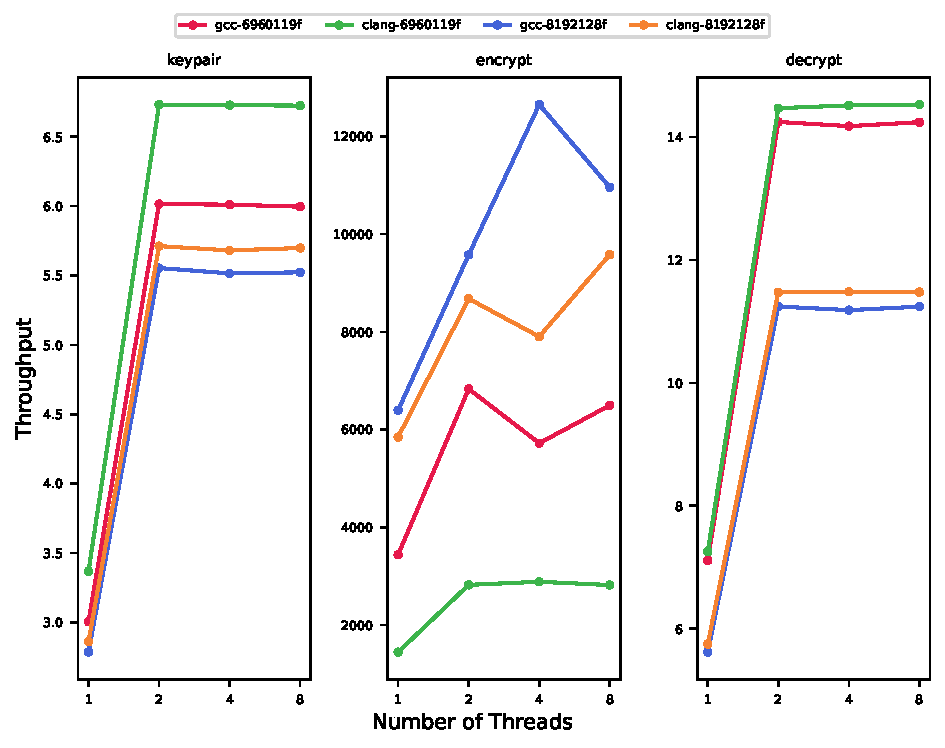
\includegraphics[scale=0.75]{chapters/results/throughput/IBM Community Cloud_mceliece.pdf}
    \caption{Throughput of \gls{mceliece} on IBM Community Cloud for Various Thread Counts}
    \label{figure:results:throughput:mceliece-ibm-community-cloud}
\end{figure} 

\begin{figure}
    \centering
    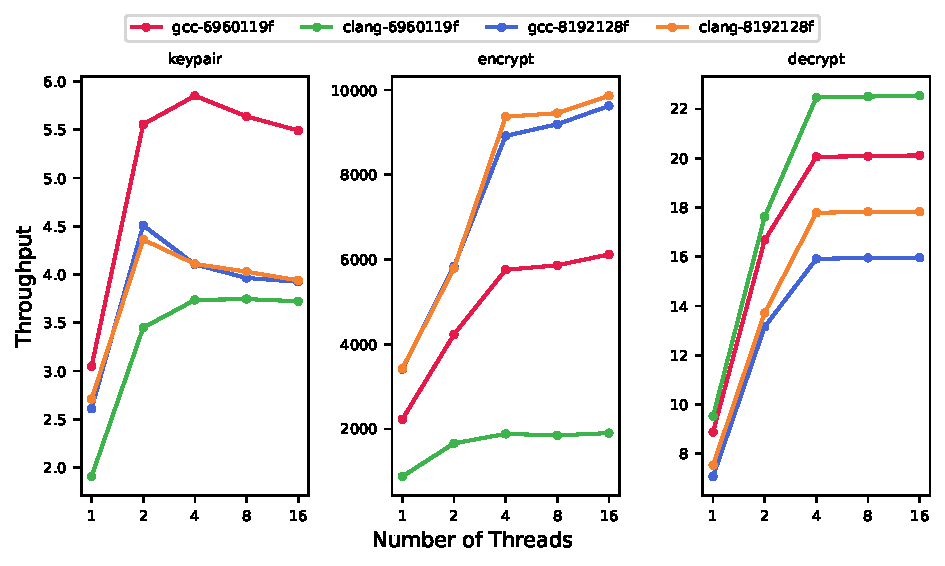
\includegraphics[scale=0.75]{chapters/results/throughput/Old Mid-Range Laptop_mceliece.pdf}
    \caption{Throughput of \gls{mceliece} on Old Mid-Range Laptop for Various Thread Counts}
    \label{figure:results:throughput:mceliece-old-mid-range-laptop}
\end{figure}

When \gls{mceliece} is run in environments with support for \gls{avx2}, such as the Modern Workstation shown in figure \ref{figure:results:throughput:mceliece:modern-workstation}, the results tell a different story. Not only are the compilers much more consistent with one another, but the difference in throughput between the two variants seem to become smaller. It is still clear to see, however, that the smallest parameter size has an overall lower throughput for keypair generation and encryption than the largest parameter size tested\todo{Is this really true? double check!}. The decrypt results seem to show that the smallest parameter size perform the best.

\begin{figure}
    \centering
    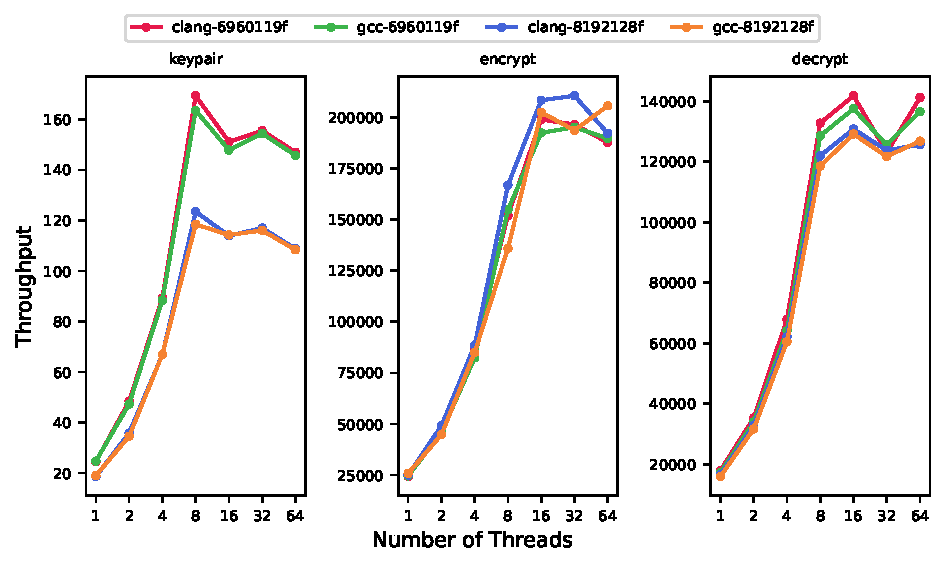
\includegraphics[scale=0.75]{chapters/results/throughput/Modern Workstation_mceliece.pdf}
    \caption{Throughput of \gls{mceliece} on Modern Workstation for Various Thread Counts}
    \label{figure:results:throughput:mceliece-modern-workstation}
\end{figure}

When running \gls{ntru} in parallel to measure throughput, we found that the performance scales well with regards to the number of threads used. In figure \ref{figure:results:throughput:ntru-modern-workstation}, \gls{ntru} HRSS 701 running in the Modern Workstation environment seems to have near-linear scaling for the thread counts tested. The variant also performs considerably better than HPS 4096821 in both the keypair generation stage and the encryption stage. The decrypt stage, however, seems to provide near identical measurements. We found that the same scaling also occurs in the Modern Laptop environment.

\begin{figure}
    \centering
    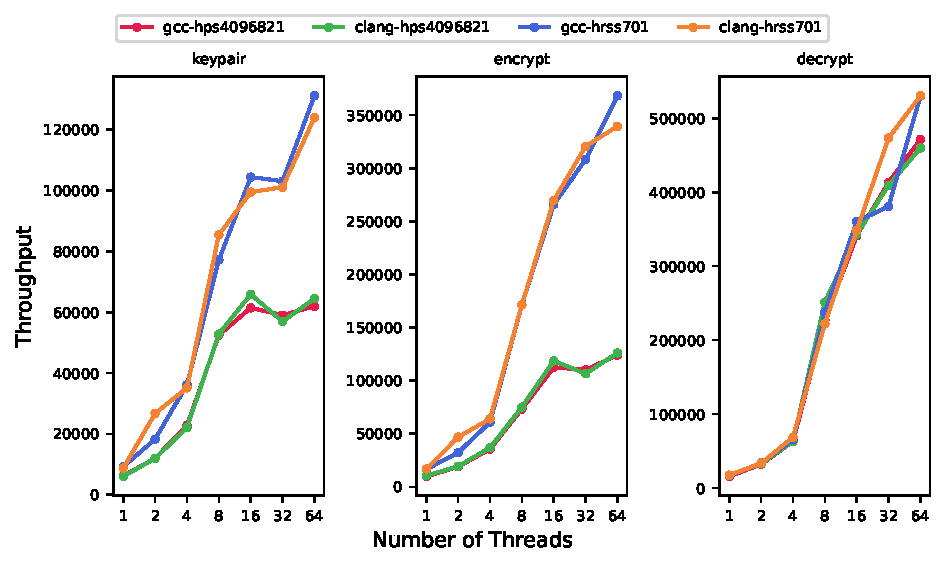
\includegraphics[scale=0.75]{chapters/results/throughput/Modern Workstation_ntru.pdf}
    \caption{Throughput of \gls{ntru} on Modern Workstation for Various Thread Counts}
    \label{figure:results:throughput:ntru-modern-workstation}
\end{figure}

In Table \ref{table:results:throughput:ntru-hrss701-decrypt}, the measurements for various compilers and thread counts are shown for all of the tested environments\todo{explain table}. The best scaling is found in the Modern Workstation environment, followed by the Modern Laptop. Although the tested cloud environments supported \gls{avx2}, they did not see the same performance increase when more threads were used. For all environments except IBM Community Cloud and Cloud Provider 2, GCC seems to produce the highest increase in throughput over the reference implementation compiled with GCC, without performance optimizations.

    \begin{table}[H]
        \centering
        \small
        \caption{Parallel Throughput Runs for ntru hrss701 (decrypt)}
        \label{table:results:throughput:ntru-hrss701-decrypt}
        \begin{tabularx}{\linewidth}{X c c c c c c c c}
            \toprule
            \thead{Environment} & \thead{Compiler} & \multicolumn{7}{c}{\thead{Threads}}\\
            & & 1 & 2 & 4 & 8 & 16 & 32 & 64 \\
            \midrule
\multirowcell{4}{Cloud\\ Provider\\ 1 \footref{avx2-optimized}} & 
\multirow{2}{*}{gcc} & 47064 & 94918 & 94690 & 101730 & 103827\\
 & & 1.0 & 2.02 & 2.01 & 2.16 & 2.21\\
\cmidrule[0.05em](){3-9} & 
\multirow{2}{*}{clang} & 39753 & 71637 & 82847 & 85968 & 85693\\
 & & 0.84 & 1.52 & 1.76 & 1.83 & 1.82\\
            \midrule
\multirowcell{4}{Cloud\\ Provider\\ 2 \footref{avx2-optimized}} & 
\multirow{2}{*}{gcc} & 33224 & 68890 & 74596 & 64194\\
 & & 1.0 & 2.07 & 2.25 & 1.93\\
\cmidrule[0.05em](){3-9} & 
\multirow{2}{*}{clang} & 39840 & 69277 & 62418 & 75534\\
 & & 1.20 & 2.09 & 1.88 & 2.27\\
            \midrule
\multirowcell{4}{IBM\\ Community\\ Cloud \footref{ref-optimized}} & 
\multirow{2}{*}{gcc} & 705 & 1056 & 1373 & 1401\\
 & & 1.0 & 1.50 & 1.95 & 1.99\\
\cmidrule[0.05em](){3-9} & 
\multirow{2}{*}{clang} & 881 & 1772 & 1735 & 1745\\
 & & 1.25 & 2.51 & 2.46 & 2.47\\
            \midrule
\multirowcell{4}{Modern\\ Laptop \footref{avx2-optimized}} & 
\multirow{2}{*}{gcc} & 14694 & 26965 & 94495 & 147789 & 172734 & 176251\\
 & & 1.0 & 1.84 & 6.43 & 10.06 & 11.75 & 11.99\\
\cmidrule[0.05em](){3-9} & 
\multirow{2}{*}{clang} & 13041 & 32001 & 87645 & 104470 & 148045 & 166157\\
 & & 0.89 & 2.18 & 5.96 & 7.11 & 10.07 & 11.31\\
            \midrule
\multirowcell{4}{Modern\\ Workstation \footref{avx2-optimized}} & 
\multirow{2}{*}{gcc} & 16668 & 33956 & 65296 & 237728 & 360264 & 380808 & 530159\\
 & & 1.0 & 2.04 & 3.92 & 14.26 & 21.61 & 22.85 & 31.81\\
\cmidrule[0.05em](){3-9} & 
\multirow{2}{*}{clang} & 17454 & 33662 & 68787 & 222164 & 348442 & 473293 & 530368\\
 & & 1.05 & 2.02 & 4.13 & 13.33 & 20.90 & 28.39 & 31.82\\
            \midrule
\multirowcell{4}{Old\\ Low-Range\\ Laptop \footref{ref-optimized}} & 
\multirow{2}{*}{gcc} & 688 & 1286 & 1492 & 1476 & 1489\\
 & & 1.0 & 1.87 & 2.17 & 2.14 & 2.16\\
\cmidrule[0.05em](){3-9} & 
\multirow{2}{*}{clang} & 583 & 1102 & 1222 & 1219 & 1218\\
 & & 0.85 & 1.60 & 1.77 & 1.77 & 1.77\\
            \midrule
\multirowcell{4}{Old\\ Mid-Range\\ Laptop \footref{ref-optimized}} & 
\multirow{2}{*}{gcc} & 873 & 941 & 1762 & 1748 & 1781\\
 & & 1.0 & 1.08 & 2.02 & 2.00 & 2.04\\
\cmidrule[0.05em](){3-9} & 
\multirow{2}{*}{clang} & 767 & 1299 & 1512 & 1515 & 1518\\
 & & 0.88 & 1.49 & 1.73 & 1.73 & 1.74 \\
            \bottomrule
        \end{tabularx}
    \end{table}
    \addtocounter{footnote}{1}
    \footnotetext{\label{ref-optimized}ref-optimized}
    \addtocounter{footnote}{1}
    \footnotetext{\label{avx2-optimized}avx2-optimized}
    

\subsection{Micro-benchmarks}

In section \ref{section:method:experiment:phase1:implementation-configurations} it was written that the monitored functions for the micro benchmark would be based off of data found in the hot paths analysis. In the end, the functions presented in Table \ref{table:results:performance:micro-functions} were monitored during the micro benchmark. Note that although the randombytes function is available in both \gls{ntru} and \gls{mceliece}, it was found in section \ref{section:results:hot-paths} to not be significant enough to warrant further analysis.

\begin{table}[H]
    \centering
    \small
    \caption{Monitored Functions}
    \label{table:results:performance:micro-functions}
    \begin{tabularx}{\linewidth}{l X}
        \toprule
        \thead{Name} & \thead{Description} \\
        \midrule
        \multicolumn{2}{c}{\thead[l]{\gls{mceliece} and \gls{ntru}}} \\
        %\midrule
        crypto\_kem\_keypair & Generate a keypair \\
        crypto\_kem\_enc & Generate and encapsulate a key \\
        crypto\_kem\_dec & Decapsulate an encapsulated key \\
        \midrule
        \multicolumn{2}{c}{\thead[l]{\gls{mceliece}}} \\
        pk\_gen & Generate the public-key\\
        gen\_e & Generate an error vector of a specific weight (encryption)\\
        syndrome & Create the syndrome using the public key and an error vector (encryption)\\
        % syndrome\_asm & The same as syndrome, but implemented in assembly targeting AVX2\\
        root & A polynomial at one or more field elements are evaluated (decryption)\\
        synd & Syndrome computation (decryption)\\
        \midrule
        \multicolumn{2}{c}{\thead[l]{\gls{ntru}}} \\
        poly\_Rq\_mul & Multiply a polynomial with another in $\mathbb{R}_q$\\
        poly\_S3\_inv & Invert a polynomial in $\mathbb{S}_3$\\
        randombytes & Retrieve uniformly random bytes \\
        poly\_Rq\_inv & Invert a polynomial in $\mathbb{R}_2$\\
        poly\_R2\_inv & Invert a polynomial in $\mathbb{R}_2$\\
        poly\_R2\_inv\_to\_Rq\_inv & Lift an inverted polynomial from $\mathbb{R}_2$ to $\mathbb{R}_q$ \\
        poly\_Sq\_mul & Multiply a polynomial in $\mathbb{S}_q$ with another\\
        \bottomrule
    \end{tabularx}
\end{table}
\todo[inline]{gf\_add, gf\_mul missing from the measurements due to extreme overhead? Several millions of invocations too much for perf?}

To evaluate what changes in the implementations contribute to a certain speedup, micro-benchmarks were run as further described in section \ref{section:method:experiment:phase1}. One of the micro-benchmarks performed was the counting of the number of cache misses occurring in an environment. The cache misses for various environments and performance optimizations for \gls{mceliece} 8192128f keypair generation is presented in Table \ref{table:results:micro:cache-misses-mceliece-8192128f-enc}. The same stage for the \gls{ntru} HRSS 701 implementations tested are presented in Table \ref{table:results:micro:cache-misses-ntru-hrss701-enc}. In both of the tables, the Old Low-Range Laptop is missing for some configurations, due to it failing to complete the micro benchmarks a multitude of times. Not all environments supported measuring the cache misses. Therefore the Cloud Provider 1 and IBM Community Cloud are not presented in the following tables.

The number of cache misses in \gls{mceliece}, when compared to \gls{ntru}, is substantially higher with comparable means being up to 190 times as many. The standard deviation is also considerably higher than those found in \gls{ntru} benchmarks. Despite running several generations older hardware with less then half the cache of the Modern Laptop, the Old Low-Range Laptop seem to consistently have fewer cache misses. The only cloud hardware tested, Cloud Provider 2, has an unknown amount of cache available for use during the benchmark, it being a shared environment with virtual cores. The Cloud Provider 2 saw an increased number of cache misses when compared to dedicated consumer hardware such as the Old Mid-Range Laptop, the Old Low-Range Laptop and the Modern Workstation environments.

\begin{table}[H]
    \centering
    \small
    \caption{Cache Misses in the Encryption Stage of \gls{mceliece} 8192128f}
    \label{table:results:micro:cache-misses-mceliece-8192128f-enc}
    \begin{tabularx}{\linewidth}{l c c c c c c}
        \toprule
        \thead{Environment} & \thead{Compiler} & \thead{Flags} & \thead{Mean} & \thead{Standard\\Deviation} & \multicolumn{2}{c}{\thead{95\% CI}}\\
        & & & & & \thead{Lower} & \thead{Upper} \\
        \midrule
               Modern Laptop &                  gcc &                  ref &                32211 &                 8953 &                31819 &                32604\\
               Modern Laptop &                  gcc &        ref-optimized &                 1849 &                 5766 &                 1596 &                 2102\\
               Modern Laptop &                  gcc &                 avx2 &                 1225 &                 4118 &                 1044 &                 1406\\
            Cloud Provider 2 &                  gcc &       avx2-optimized &                 1652 &                 3130 &                 1515 &                 1789\\
               Modern Laptop &                  gcc &       avx2-optimized &                  816 &                 3069 &                  681 &                  950\\
               Modern Laptop &                clang &        ref-optimized &                  716 &                 2326 &                  614 &                  818\\
               Modern Laptop &                clang &       avx2-optimized &                  657 &                 2306 &                  556 &                  758\\
            Cloud Provider 2 &                  gcc &        ref-optimized &                21023 &                 2147 &                20929 &                21117\\
        Old Mid-Range Laptop &                  gcc &        ref-optimized &                 1545 &                 1359 &                 1485 &                 1604\\
            Cloud Provider 2 &                  gcc &                 avx2 &                  602 &                 1335 &                  543 &                  661\\
            Cloud Provider 2 &                clang &       avx2-optimized &                  345 &                 1260 &                  290 &                  400\\
            Cloud Provider 2 &                  gcc &                  ref &                22037 &                  826 &                22001 &                22074\\
        Old Low-Range Laptop &                  gcc &        ref-optimized &                 1185 &                  788 &                 1136 &                 1234\\
        Old Mid-Range Laptop &                  gcc &                  ref &                 3092 &                  712 &                 3061 &                 3124\\
            Cloud Provider 2 &                clang &        ref-optimized &                  108 &                  674 &                   78 &                  137\\
        Old Mid-Range Laptop &                clang &        ref-optimized &                  685 &                  337 &                  670 &                  700\\
        Old Low-Range Laptop &                  gcc &                  ref &                  771 &                  264 &                  759 &                  782\\
        Old Low-Range Laptop &                clang &        ref-optimized &                  455 &                  147 &                  446 &                  464\\
          Modern Workstation &                clang &        ref-optimized &                    3 &                   50 &                    1 &                    6\\
          Modern Workstation &                  gcc &                  ref &                    4 &                   49 &                    1 &                    6\\
          Modern Workstation &                  gcc &        ref-optimized &                    1 &                   12 &                    0 &                    1\\
          Modern Workstation &                clang &       avx2-optimized &                    0 &                    2 &                    0 &                    0\\
          Modern Workstation &                  gcc &                 avx2 &                    0 &                    2 &                    0 &                    0\\
          Modern Workstation &                  gcc &       avx2-optimized &                    0 &                    1 &                    0 &                    0\\
        \bottomrule
    \end{tabularx}
\end{table}

With an average of 6911670 cache misses when the GCC reference implementation was run in the Cloud Provider 2 environment, keypair generation in \gls{mceliece} 8192128 had the largest number of cache misses recorded during our testing. For the same algorithm and compiler configuration, the Modern Workstation had an average of 20403 cache misses. In the other end of the spectrum, the Modern Workstation saw an average of a single cache miss for all configurations of \gls{ntru} HPS 4096821 keypair generation. Using the same configurations, the Cloud Provider 2 environment saw an average of between 1440 and 3468 cache misses. 

That the \gls{mceliece} implementations had a drastically larger amount of cache misses than the \gls{ntru} implementations was found in all of the tests of the experiment.

\begin{table}
    \centering
    \small
    \caption{Cache misses in the encryption stage of \gls{ntru} HRSS 701}
    \label{table:results:micro:cache-misses-ntru-hrss701-enc}
    \begin{tabularx}{\linewidth}{l c c c c c c}
        \toprule
        \thead{Environment} & \thead{Compiler} & \thead{Flags} & \thead{Mean} & \thead{Standard\\Deviation} & \multicolumn{2}{c}{\thead{95\% CI}}\\
        & & & & & \thead{Lower} & \thead{Upper} \\
        \midrule
               Modern Laptop &                  gcc &                  ref &                  169 &                  318 &                  155 &                  183\\
            Cloud Provider 2 &                  gcc &       avx2-optimized &                  123 &                  210 &                  114 &                  132\\
               Modern Laptop &                clang &       avx2-optimized &                   51 &                  170 &                   44 &                   59\\
               Modern Laptop &                clang &        ref-optimized &                   67 &                  164 &                   60 &                   74\\
               Modern Laptop &                  gcc &                 avx2 &                   43 &                  163 &                   36 &                   50\\
               Modern Laptop &                  gcc &       avx2-optimized &                   49 &                  159 &                   42 &                   56\\
               Modern Laptop &                  gcc &        ref-optimized &                   64 &                  158 &                   57 &                   71\\
            Cloud Provider 2 &                clang &        ref-optimized &                   76 &                   94 &                   72 &                   80\\
            Cloud Provider 2 &                  gcc &        ref-optimized &                   78 &                   93 &                   74 &                   82\\
            Cloud Provider 2 &                clang &       avx2-optimized &                   72 &                   79 &                   69 &                   76\\
            Cloud Provider 2 &                  gcc &                 avx2 &                   45 &                   74 &                   42 &                   49\\
            Cloud Provider 2 &                  gcc &                  ref &                   86 &                   72 &                   83 &                   89\\
        Old Mid-Range Laptop &                  gcc &                  ref &                   28 &                   42 &                   26 &                   30\\
        Old Mid-Range Laptop &                  gcc &        ref-optimized &                    7 &                   22 &                    6 &                    8\\
        Old Mid-Range Laptop &                clang &        ref-optimized &                    7 &                   18 &                    6 &                    8\\
        Old Low-Range Laptop &                  gcc &                  ref &                    2 &                   18 &                    1 &                    3\\
        Old Low-Range Laptop &                clang &        ref-optimized &                    1 &                    4 &                    1 &                    1\\
        Old Low-Range Laptop &                  gcc &        ref-optimized &                    1 &                    3 &                    0 &                    1\\
          Modern Workstation &                clang &       avx2-optimized &                    0 &                    2 &                    0 &                    0\\
          Modern Workstation &                  gcc &       avx2-optimized &                    0 &                    1 &                    0 &                    0\\
          Modern Workstation &                  gcc &                 avx2 &                    0 &                    1 &                    0 &                    0\\
          Modern Workstation &                  gcc &                  ref &                    0 &                    1 &                    0 &                    0\\
          Modern Workstation &                  gcc &        ref-optimized &                    0 &                    1 &                    0 &                    0\\
          Modern Workstation &                clang &        ref-optimized &                    0 &                    1 &                    0 &                    0\\
        \bottomrule
    \end{tabularx}
\end{table}

% Discussion
% \chapter{Discussion}
\label{chapter:discussion}

\section{Post-Quantum Cryptography on IBM Z}

As mentioned in~\cite{microsoft2020, ibm:z15:2019}, the fact that current hardware provides cryptographic agility is important as the \gls{post-quantum} standard evolves. By providing users with the ability to update the firmware of \glspl{hsm} as well as adding user defined extensions, we believe it is likely that the \gls{nist} submissions may be implemented efficiently on the \glspl{hsm} as the algorithms mature.

The IBM 4769 \gls{hsm} supports \gls{dilithium}, a lattice-based signature algorithm. The implementation is not entirely clear, but it is assumed to be implemented in the \gls{asic}. It is unclear whether or not the functions of the \gls{dilithium} implementation is split, allowing other lattice-based cryptosystems to be implemented using the acceleration offered by the \gls{asic}. If such an implementation was possible via an extension, we assume that the performance increase would be considerate when compared to software-based implementations, given the nature of the \gls{asic} implementations. Even if other lattice-based cryptosystems could not make use of the \gls{asic}, the \gls{fpga} integrated in the \gls{hsm} should in theory offer a significant speedup for \gls{post-quantum} \glspl{kem}~\cite{zhu2021, roy2020}. We believe that, due to the seemingly lack of low-level primitives for lattice-based crypto on IBM's \glspl{hsm}, it is unlikely that we would be able to see an increase in performance of the \gls{post-quantum} \glspl{kem}. Given a study of \gls{fpga} implementations, however, one could expect to see a considerable increase in throughput.

Though we were unable to utilize IBM's \gls{hsm} offerings, we believe that they would significantly increase the speed of the classical algorithms \gls{ecdhe} and \gls{dhe} as the \glspl{hsm} support these algorithms. Even without using the \glspl{hsm}, we did see a significant increase in performance for the \gls{ecdhe} due to its support for \gls{ecc} in \gls{cpacf}. In our parallel benchmarks for measuring the throughput of the classical algorithms, we saw a peak throughput of 100000 keypairs and 20000 \gls{ecdhe} exchanges when using the \gls{x25519} algorithm. We believe that these results give a glimpse of what's possible when successfully targeting the \gls{z15} platform. 

As seen in section \ref{section:results:z15}, the 4769 \gls{hsm} supports \gls{aes}, \gls{sha3} and random number generation. These algorithms were identified to be of importance when it comes to performance tuning of \gls{post-quantum} \glspl{kem}. In the case of some lattice-based \glspl{kem} it was found that a majority of the computation time was spent using \gls{sha3} functions. We therefore believe that by utilizing these primitives as drop-in replacements in the studied implementations, one could expect a significant performance increase. We were not able to put this theory to the test as we were unable to get access to IBM's \gls{hsm} offerings.

IBM \gls{z15} features \gls{simd} operations at 5.2GHz. Based on the literature we have studied, it seems unlikely that the \gls{z15} suffers from the same downclocking when performing \gls{simd} operations as \gls{avx2} on Intel processors. As such, we believe that \gls{simd} implementations on \gls{z15} would result in a higher throughput than a comparable implementation run on consumer or cloud hardware. We found that the \gls{avx2} implementations studied provided inconsistent throughputs. We believe that this, in part, has to do with the aforementioned downlocking of the CPU core when performing \gls{avx} operations on Intel hardware as previously described in section \ref{section:background:simd-avx}. If the stability of \gls{simd} operations on \gls{z15} performs at sustained 5.2GHz, the performance would most likely outperform that of comparable Intel machines.

The use of \gls{simd} instructions on \gls{z15} is a topic we had to omit in this paper due to time constraints. As all of the vectorized \gls{nist} submissions used \gls{avx2} in several thousands of lines of assembly, we found it difficult to efficiently study their implementations and translate them for use on \gls{z15}. Though vector intrinsics would provide us with a more efficient way of translating the implementations for use on \gls{z15}, none of the implementations studied had provided such an implementation in their submission or elsewhere. A more automatic approach would be to use IBM XL which features an automatic conversion of code to \gls{simd} instructions, where applicable~\cite{ibm:xl-autosimd}. We were however unable to access IBM XL due to its licensing cost and as such our results largely rely on non-vectorized code when running on \gls{z15}.

IBM have invested in making Z a quantum safe platform~\cite{ibm:z15:2019} and as such we believe they will continue focus on improving the performance and security of the \gls{post-quantum} \glspl{kem} implementations they offer today and in the future. Based on literature, we have identified that a high-performance \gls{post-quantum} \gls{kem} implementation relies on high-performance \gls{sha3} implementations, random number generation and polynomial arithmetic. By offering hardware-based support for these features, as well as by introducing hardware-accelerated polynomial primitives such as polynomial multiplication, we believe that IBM would further assert the potentials the performance of \gls{post-quantum} \glspl{kem} on Z. In terms of polynomial multiplication, the use of \glspl{ntt} or Karatsuba algorithms was found to be dominant in the algorithms submitted to \gls{nist}. By providing such implementations in hardware, polynomial multiplication could be further optimized.

One complaint regarding the performance of \gls{simd} instructions on hardware with support for \gls{avx2} has been the limited number of vector registers - 16 256-bit registers per processor~\cite{guneysu2013}. The \gls{z15} processor has 32 128-bit registers per processor~\cite{redbook:z15}, meaning that it does not offer a better set of registers than other hardware. As seen in section \ref{section:results:z15}, the low count of available \gls{simd} registers means that an increased number of load and store operations will be required~\cite{guneysu2013}. As we have been unable to find literature comparing the load and store operations performance of \gls{z15} and other hardware, we believe more work is required on the topic to analyze the performance impacts of \gls{post-quantum} \glspl{kem} in that regard.

\todo[inline]{
Minnessäkerhet
We have not focused on memory security in this blabbasd.... IBM memory security...

Cache-storlekar. L3 på Z är gigantisk, våra egna resultat verkar tyda på att cache kan vara viktigt.

Argue that some cryptos use 16-bit, others 64-bit. It may be important. For crypto agility we need both?
}

\section{Readiness for the Post-Quantum Transition}

Jacobi and Webb~\cite{jacobi2020} claim that mainframes process 90\% of the world's credit card transactions. This sensitive information must be kept secure. Therefore one may argue that the transition to post-quantum cryptography needs to happen earlier in the banking sector than in other sectors. A question one may then ask them self is, how would the transition to post-quantum cryptography affect mainframe users? Our data suggests that the performance hit would be severe, especially on mainframe hardware. Mainframes have an outstanding \gls{ecdh} performance because it takes advantage of the \gls{cpacf} co-processor to accelerate the calculations. But \gls{cpacf} does not support any of the post-quantum cryptographic algorithms. After \gls{nist}'s standardization process is finished, IBM should consider adding support for the standardized algorithms on the \gls{cpacf} to alleviate the performance impact of the transition. Furthermore, could IBM add support for it in their cryptocards.

Suppose we have a scenario where we replace the \gls{ecdhe} algorithm in \gls{tls} 1.2 with \gls{kem} and keep everything else unchanged. Then consider a using requesting a website such as a search engine. Note that this is only a theoretical scenario; in reality, further parts will likely be changed to accommodate the \gls{post-quantum} \glspl{kem}. Further, the best case will be used in this scenario - the most optimized versions of the algorithms running on a modern workstation. How would the performance of \gls{tls} be affected? If we replace \gls{ecdhe} with \gls{mceliece} 6960119f, the client will notice an extra delay of about 80 ms, about 800 times slower than today. For the server, this will significantly lower the throughput. If we replace \gls{ecdhe} with \gls{ntru} HPS 4096821, the extra delay is about 0.3 ms, around 4 times slower, probably not noticeable for a client. But for a server handling thousands of requests a second, the transition to post-quantum will be prominent. It is not yet clear if one will be required to generate a new key for every transaction when switching to \glspl{kem} from the traditional \glspl{kex}. If it is not required, we may remove the key generation time from the calculation. The extra delay could be cut down to about 0.1 ms and 0.05 ms for \gls{mceliece} and \gls{ntru}, respectively. We can see that \gls{mceliece} is slower in comparison to \gls{ntru}, but we need to take into account that \gls{mceliece} 6960119f has a higher security level.

To make implementations of cryptos more cross-platform, one may use vector-based intrinsics. The support for these varies between platforms, however. For example, \gls{ibmz} only supports a limited range of the functions. In order to effectively rely on vector intrinsics, we would need a standard that all platforms have support for. A problem with using intrinsics is that it can be hard to ensure constant time operations over multiple platforms. Because the intrinsics would be compiled into different instructions for each architecture, this is also true for the IBM XL AutoSIMD feature that can convert \gls{avx} to \gls{ibmz} \gls{simd} instructions.

\section{The Performance of Post-Quantum Key Encapsulation Mechanisms}

% mceliece - teoretiskt (enligt författarna) sätt är icke-f snabbare än f - men i praktiken är det verkligen inte så. icke-f mycket icke-determinstiskt
According to the \gls{nist} submission of Albrecht et. al.~\cite{mceliece2020}, the systematic (non-f) variant of \gls{mceliece} theoretically performs better during key generation than the semi-systematic (f) variant as it requires less computational work per key-generation attempt. They further state that this is true for as long as the systematic variant succeeds in finding a valid key with as few tries as possible. In reality, we found that the systematic variant consistently performs worse than the semi-systematic variant. Although theoretically faster, it seems as if the key generation of the systematic variant requires more tries than the authors anticipated. We further found that the systematic variant performs considerably more non-deterministically with a larger standard deviation than that of the semi-systematic variant. Although the implementation provided by the authors of the \gls{nist} submission is not yet standardized, we believe that one should pursuit the semi-systematic variant of \gls{mceliece} if \gls{nist} decides on standardizing it - if solely taking performance into account. Albrecht et. al. further discuss that it is unknown if the performance gain of the semi-systematic variant warrants its more complicated implementation or if users will even benefit from the speedup. As we found that the semi-systematic \gls{mceliece} variant 8192128f performed more than three times as fast as the systematic reference implementation and almost two times as fast as the systematic \gls{avx2} implementation, we believe that the more complex semi-systematic form is indeed warranted when only considering the performance of the \gls{kem}.

%%% === TODO LARGE CHANGE IN TOPIC HERE === %%%
% Cloud hardware - dip in performance over time. Counter argument - cloud provider 1 not behaving the same?
When performing our tests on cloud hardware, we anticipated a less consistent result than on dedicated consumer hardware. We believed that, due the virtualized and shared nature of the resources, the cloud environments would yield varied results over time as other users of the system utilized the hardware. We found that the Cloud Provider 2 environment had several performance discrepancies over time when running \glspl{kem} in sequential iterations. We also found, however, that Cloud Provider 1 largely functioned as the dedicated consumer hardware we tested. Although it is difficult to conclude from the small sample of cloud providers in our tests, we argue that there is in fact a non-zero chance that virtualized cloud hardware performs less consistently than dedicated hardware, given that Cloud Provider 2 had performance discrepancies in all of our sequential benchmarks. 

% Modern Laptop - Cache misses, oregelbundna minnesaccess
Another phenomena found in our data is how the Modern Laptop environment consistently yields the largest number of cache misses. Despite having a considerably newer CPU and more available cache than the Old Mid-Range Laptop and the Old Low-Range Laptop, the Modern Laptop environment performed much worse, as seen in Tables \ref{table:results:micro:cache-misses-mceliece-8192128f-enc} and \ref{table:results:micro:cache-misses-ntru-hrss701-enc}. We believe that this is due to the agressive prefetch mechanisms found in newer CPUs. These mechanism could badly predict what memory is necessary for future computation and as such evict memory that is used by the algorithms we benchmarked. The older machines could have less agressive mechanisms, or lack them all together, leading to fewer faults. We believe that this prefetching of cache did not constitute an issue for the Modern Workstation as it had double the amount of cache, resulting in virtually zero cache misses across the board.

%%% === TODO LARGE CHANGE IN TOPIC HERE === %%%
% -- mceliece använder betydligt mycket mer minne än övriga algoritmer - inte lämpligt för IoT etc?
When considering the memory footprint of the proposed \glspl{kem}, one must take into account the stack usage, heap usage as well as the parameter sizes of the algorithms. We found that the heap usage of the algorithms is negligible. The parameter sizes, however, vary considerably between \gls{mceliece} and \gls{ntru}. \gls{mceliece} requires between one and one point three megabytes of memory to store a public key, whilst \gls{ntru} requires a hundredth of that - roughly 1000 bytes. Although \gls{mceliece}'s private key is considerably smaller, it is still ten times as large as \gls{ntru}'s private key at roughly 13KiB. We therefore believe that \gls{mceliece} is impractical for use in low-memory environments such as embedded devices.

%%% === TODO LARGE CHANGE IN TOPIC HERE === %%%
% -- ntru skalar mycket bättre än mceliece sett till trådar
The data we collected for throughput and scaling of the algorithms identified that none of the classical algorithms scaled well when increasing the number of threads that concurrently executed the algorithms. In fact, it seemed as if the worst scaling and throughput was found in \gls{dhe}, followed by \gls{mceliece}. The algorithms saw virtually no increase in throughput once the number of threads surpassed the number of cores of the system. The performance of \gls{ecdhe} varied depending on the environment it was run in, but in general, the scaling was better than that of \gls{dhe}, with improvements made beyond the system's core count. The best scaling by far was found in the AVX2 optimized \gls{ntru} HRSS 701 implementations that saw a near-linear increase in performance with regards to the number of threads - even when passing the core count of the machine itself. Furthermore, the scaling of \gls{ntru} HRSS 701 was found to be the best in Modern Laptop and Modern Workstation, with the latest CPUs included in the test. We therefore strongly believe that \gls{ntru} HRSS 701 is a top candidate for \gls{post-quantum} \glspl{kem}, when only considering performance. Although not strictly comparable, we believe that one may expect similar performance of \gls{ntru} and the classical \gls{ecdhe}, judging from our measurements of throughput and scaling.

\todo[inline]{
-- argue that non-openssl aes is better due to less memory use?
}

\section{The Security of Post-Quantum Key Encapsulation Mechanisms}

% -- ntru mycket snabbare än mceliece, men säkerhetskategorin är lägre. HRSS 701 snabbare än HPS4096821, men säkerhetsnivån är lägre.
Our study has disregarded the security of the \gls{nist} submissions, letting us focus on the performance of the algorithms. It goes without saying that the security of the algorithms is of upmost importance. As we have not performed a study of the security of the algorithms on our own, we rely on the information presented by the \gls{nist} submissions themselves. As presented in \ref{table:background:submissions-security-level}, all of the \gls{mceliece} variants we tested are security level 5. The security level of \gls{ntru} varies between 3 and 5 for the HPS 4096821 variant and between 1 and 3 for the HRSS 701 variant, depending on the locality model used. We found that the HRSS 701 variant of \gls{ntru} overall performed the best out of all \gls{kem} algorithms tested. We further found that \gls{mceliece} variants performed the worst. We therefore believe, given our results, that there may be a correlation between the performance and security level of \gls{post-quantum} algorithms.

Although one may believe our sample set is small, we argue that one has to consider the broader picture. As mentioned in~\cite{ntru2020}, HPS 4096821 and HRSS 701 originated from two different \gls{nist} submissions. We therefore believe that, in part, these algorithms are different from one another - further increasing the size of the sample set. We do believe, however, that a further study of the correlation is required to definitively state whether or not there is a correlation between the security level of an algorithm and its performance.

% -- Återkoppla till säkerhetskategorierna - kategori 1 är AES128.
% -- Koppla ihop med Grover - AES 256 blir teoretiskt AES 128, vilket gör säkerhetsnivån halveras. I praktiken påstår nist2017 att det inte är ett problem - då den är svår att köra. Teoreitskt kan det då vara ett måste med kategori 5.
As described in section \ref{section:background:security-categories}, the categories are largely based on the strength of classic block-ciphers. Security category 1, for example, is defined based on attacks on AES 128. The fifth and strongest security category, category 5, is defined based on attacks on AES 256. These definitions, as well as the implications of Grover's algorithm described in section \ref{section:background:classical-cryptography-threats}, could result in the categories being redefined if Grover's algorithm becomes practical. Such a redefinition could result in category 5 post-quantum to be as strong as category 1 pre-quantum. That is, one may argue that only category 5 algorithms should be considered true post-quantum algorithms.

\section{On Performance Measurements}

% -- diskutera skillnader i våra mätvärden och NIST submissions. SUPERCOP estimerar, beter sig icke-deterministiskt, vi räknar?.
When studying previous work before outlining the method of this thesis, we identified that \gls{supercop} seemed to be the de-facto tool for measuring the performance of cryptographic algorithms. It was referenced and used in both the \gls{mceliece}~\cite{mceliece2020} and the \gls{ntru}~\cite{ntru2020} submissions to \gls{nist}. When studying the source code, we found several areas of concerns which led us to not use the software. One of the reasons was the use of older versions of the \gls{nist} submissions. We were interested in the third round of submissions, whilst \gls{supercop} provided the implementations of the second round. Another reason which contributed to our disregard of \gls{supercop} was the use of the estimated number of CPU cycles performed as the performance measurement. We identified that the code relied heavily on using the elapsed time and the base frequency of the CPU to calculate the number of required CPU cycles. As we were interested in high-quality measurements of not only CPU-cycles, but also instruction counts, cache misses etcetera, we found the Linux kernel API to be more apt for our use case. As it uses the hardware counters found in many CPUs, we argue that our measurements are accurate since they are counted and not calculated, as is the case in \gls{supercop}. Not only did we find the use of perf leading to more deterministic results, but the number of CPU cycles we measured were overall higher than the values found in the \gls{nist} submissions, as presented in Table \ref{table:results:sequential:nist-vs-ours}. We argue that the use of estimated CPU cycles yields inaccurate results which may easily be affected by many variables of the environment, such as the base clock of the CPU. The \gls{supercop} user guide recommends that one disable both hyper-threading and boosting so that it may more accurately calculate the number of CPU cycles~\cite{supercop}. We believe that it is not a common practice in reality to turn off both hyper-threading and boosting, which led us to use both technologies in our measurements. To decrease the risk of environmental factors such as boosting to affect our measurements, we repeated all of the measurements up to a thousand times per benchmark. We also repeated the entire benchmark at two completely different occasions. We argue that a method of measuring the performance, such as the one used by us in this thesis, would provide the public with more accurate and real-world values regarding the performance of the cryptographic algorithms. Despite us using the Linux kernel perf API, we believe that there are valid reasons use \gls{supercop}'s method of measuring CPU cycles. The Linux kernel API requires hardware support in order to accurately measure CPU cycles, instruction counts etcetera. This led us to not be able to accurately benchmark all environments with regards to the CPU cycle count. \gls{supercop}'s solution, however, is less hardware-dependant and as such more suitable for cross-platform measurements on non-Intel hardware and non-Linux operating systems. To help researchers and users achieve more accurate performance measurements, we believe that the industry as a whole could benefit from the addition of hardware-based performance counters in more processor architectures and models.

% i3:a, i7:a på ntru-körningar, xeon på mceliece, svårt att jämföra?
Comparing the performance of the \gls{nist} submissions was further complicated by the wide variety of hardware used. The \gls{ntru} submission~\cite{ntru2020} used a 3.2 GHz Intel Core i3-6100T for running the reference implementation. The same submission then used an Intel Core i7-4770k to run the AVX2 implementation. The \gls{mceliece} submission~\cite{mceliece2020} used an Intel Xeon E3-1275 v3 for its performance measurements. Although we tested a wide range of hardware, we were unable to use the same hardware as the authors. We argue that the fact that a single system was not used for all of the performance benchmarks complicate the comparisons in performance. For example, the Intel Core i3-6100T has 3MB cache~\cite{i36100t} and the Xeon E3-1275 v3 8MB~\cite{xeon31275}. As we found that the number of cache misses were considerably reduced when the available cache was increased, we believe that it is entirely possible for the performance measurements presented in the \gls{ntru} submission to be considerably worse than if they would have used the same environment as the \gls{mceliece} submission. In part, one may argue that this issue is up to \gls{nist} to solve before considering the standardization of an algorithm, but we believe it makes for a more difficult comparison when such a variety of hardware is used to represent the algorithms' performance no matter the stage of the submissions.

% mceliece Ours: ref-optimized modern workstation, theirs Intel  Xeon ref -O3 etc...
% ntru: ours ref-optimized modern workstation, theirs intel i 3-6000? etc...
% ntru ours: avx2-optimized modern ... theris i7-4770K (Haswell)
% supercop 1% av ntruhps4096821, 60% av ntruhrss701 wtf?
% amd64; CoffeeLake (906ea); 2017 Intel Core i7-8700; 6 x 3200MHz; bitvise, supercop-20190910
% https://bench.cr.yp.to/results-kem.html
% NTRU stated that their results were to be presented on the same page, but they were not

% Threats to Validity
\section{Threats to Validity}

\todo[inline]{ diskutera hur benchmarks inte säkerställer att rätt svar ges från algoritmerna. Detta utelämnas p.g.a. prestanda / träffsäkerhet i mätningar. Vi löser det genom att ha tester som är samma kod som benchmarken, fast med validering}

\todo[inline]{
-- Update after result and method changes.

-- Difficult to measure in Cloud environments - shared hosting etc.

-- Dedicated hardware for mainframes may behave differently

-- Did not use Intel C++ Compiler (ICC)

-- Did not use IBM XL
}

\subsection{Conclusion validity}

\todo[inline]{Add Conclusion validity}

\subsection{Internal validity}
\label{section:method:internal-validity}
% History - An unrelated event influences the outcomes.
Other software running on the OS may influence the results. To prevent this, we will minimize the set of programs running on the system and run the experiment multiple times at different times.

% Maturation - The outcomes of the study vary as a natural result of time.
Another factor, \gls{jit} compilation and garbage collection could influence the results. As we use the programming languages C and Assembly this will not be a problem as they do not use \gls{jit} compilation and provide full control of memory. Other programs running on the system which use JIT compilation or garbage collection falls under the previous category.

\todo{GPU kernel \gls{jit} compilation}

\todo{Swap locks the system while writing/reading to from disk}
\todo{Cache misses}

\todo{Windows Update?}

The post-quantum implementations are not final nor standardized, which may affect the performance of the implementations and the relevance of the results in the future. \gls{dhe} and \gls{ecdhe} have been standardized and optimized for many years and have mature implementations, they are likely fully optimized by this point.

% Instrumentation - Different measures are used in the pre-test and post-test phases.
We have written the measurement tools, the implementation may have shortcomings and OS differences may lead to different results. To ensure the correctness and consistency between platforms we both have reviewed the code and tested it on different platforms\todo{??????}.

%Testing - The pre-test influences the outcomes of the post-test.
Hardware can throttle because of the temperature increase caused by the benchmarks. This could result in worse performance than intended when running consecutive tests. To mitigate this, benchmarks will not be run directly after each other. We will instead wait for the temperature of the system to normalize to the same level it was before the test was started.

We cannot necessarily use the same OS for the mainframes and x86, which could cause varying results. This is however not an issue. We do not aim to pit x86 against Z, rather represent a type of computer and evaluate their readiness.

%Selection bias - Groups are not comparable at the beginning of the study.
One may argue that the choice of the two post-quantum algorithms is biased, but we argue that that point is invalid. The algorithms were selected from four finalists in round 3 of \gls{nist}'s standardization process. \gls{ntru}, \gls{crystals-kyber}, and \gls{saber} are all lattice-based algorithms, and at most one of these will be standardized. \gls{ntru} was selected based on the comment \gls{nist} gave each of the participants\todo{insert the comment?}. \gls{mceliece} was the only non-lattice-based finalist. It also has a long and good reputation\cite{nist2020}. In addition to these four finalists, there are alternate candidates still in round 3. These were not considered. The choice was made to bring down the scope to a manageable level for this work.

As has been mentioned previously, we lean heavily on \gls{nist} recommendations as they in many cases provide the authoritative recommendation of algorithms used by protocol implementers (\todo{to some extent EU paper as well????}). As we have not identified any other standardization process like that of \gls{nist}, we have concluded that relying on their expertise in this context is correct.

For the implementations of \gls{dhe} and \gls{ecdhe}, we only use the underlying algorithms provided by \gls{openssl} and \gls{openssl} with the IBM engine. This was done as \gls{openssl} was identified as the main library for these algorithms on the tested platforms. Using other libraries such as BoringSSL might have resulted in different measurements. The implementations available in \gls{openssl} have been rigorously tested and analyzed by the industry over the decades it has seen use. We are therefore confident that, although the exact measurements may differ between libraries, \gls{openssl} provides a solid foundation for our use case as a representation of today's algorithms.

\todo{We have only selected a subset of potential optimizations?}

%Attrition - Dropout from participants
\todo{Not applicable? Perhaps all subjects and platforms will not be able to see all optimizations or compiler flags?}

\subsection{Construct validity}

% Extent to which the experiment setting actually reflects the construct under study. Treatment reflects the construct of the cause well. Output reflects the construct of the effect well

% Construct validity evaluates whether a measurement tool really represents the thing we are interested in measuring. It’s central to establishing the overall validity of a method.

As previously mentioned, we are interested in measuring the following values:

\todo[inline]{These do not correspond to the ones we actually measure? Update. Also; clarify that we're measuring two different things - single iteration and multi-core.}
\begin{itemize}
    \item Encapsulation throughput in number of required CPU cycles, instruction count and wall clock time
    \item Decapsulation throughput in number of required CPU cycles, instruction count and wall clock time
    \item Keypair throughput in number of required CPU cycles, instruction count and wall clock time
    \item Hardware utilization in terms of memory (heap and stack allocation)
    \item Hardware utilization in terms of processing (logical core utilization)
\end{itemize}

For our measurements, we rely on the standard Linux kernel-based API named perf (perf\_event\_open). The API was introduced in Linux 2.6.31 which was released in 2009\footnote{\href{https://www.linux.com/news/linux-2631-released/}{https://www.linux.com/news/linux-2631-released/}}. The API has grown, and as is tradition with the Linux development, each iteration of the API has been reviewed extensively by multiple people throughout the years. We are confident that the API provides as accurate data as the kernel is able to collect.

To make the API usable, we provide a lightweight instrumentation tool which is used to measure the values as listed above. By using the C pre-processor, usage of the tool is readable and configurable and written to not introduce any overhead over the raw Linux API when performing measurements. We therefore argue that the tool does not introduce any additional risks over the base API.

By reading the official documentation of the API, we have ensured that the values we measure correspond to those we are interested in. That is, when we use the API to measure CPU cycles, for example, we have asserted that our code indeed refers to the correct measurements as described in the documentation.

\subsection{Content validity}

% Refers to the extent to which a measure represents all facets of a given construct.
%"refers to the degree to which an assessment instrument is relevant to, and representative of, the targeted construct it is designed to measure."

To answer our first research question, \textit{Does performance of post-quantum cryptography algorithms differ between architectures and if so, how?},  we do not need to measure anything other than at the start and end of the algorithm invocation. This, since the algorithm's usage will include all of the system's parts. As such, measuring the time, CPU cycles and total instructions of the entire system should suffice.

For our other research questions we examine optimizations of different parts of the algorithm. We need to see how the parts in the system as a whole are performing. For this, we will use micro-benchmarks. Micro-benchmarks may add a non-trivial overhead that depends on the number of benchmarks. We will evaluate the impact of these. We will perform the experiment once with and once without the micro-benchmarks to see the difference and make sure it is not statistically significant. If there is a significant amount of overhead, each micro-benchmark will be run in complete isolation.

When measuring memory usage, we cannot measure any other performance metric as it could induce a higher memory load unrelated to the algorithm under test. Instead, we perform the measurement of the memory usage of the key-pair generation, encryption, and decryption separate from the CPU measurements.

\todo{Measurement issues with perf - overflow or negative numbers in uint64}

\subsection{Criterion validity}
In the publications for the \gls{nist} submissions, the authors have written their own performance analysis using the \gls{supercop} benchmark tool. The presented measurements are for the total number of cycles used by the algorithms for generating keys, encapsulation and decapsulation. As these figures have not been validated by a third party, we will not use them to validate ours. We will however present comparisons in order to identify potential issue in their measurements or ours.

\subsection{External validity}

% Sampling bias.
As previously discussed under section \ref{section:method:internal-validity}, internal validity, one may argue that the selection of subjects is biased as we do not take the entire population of post-quantum and modern-day algorithms into account. Such a comparison would however be unfeasible. That is why the presented sample is based on the accumulative recommendations of several organizations. We therefore argue that our sample is representative of the algorithms that are and likely will be in use.

% History.
Another factor that may hurt the generalizability of the results is the potential of a series of unrelated events influencing the outcome. We have identified several actions to help mitigate this risk, as discussed further in section \ref{section:method:internal-validity}, internal validity.

% Experimenter effect.
The implementations used for benchmarks are not created by us. They have, however, been slightly altered in order to support various forms of optimization. This fact may result in the tested implementations performing differently than if the original implementers would have applied the optimizations. It is therefore plausible that the measurements of the samples will not be general to other implementations using the same techniques.

% Aptitude treatment.
As there are several optimization techniques such as vectorization and compiler flags applied simultaneously, there is a potential for techniques to cancel each other out or in other ways impact the performance negatively. We will mitigate this risk by evaluating each form of optimization in isolation, before combining all techniques into a truly optimized implementation.

% Situation effect.
Factors such as various settings, time of day and location may limit the generalizability of the presented findings. We have identified several mitigative actions as defined under \ref{section:method:internal-validity}, internal validity.

% Counter threats.
To counter threats across the experiment we aim to improve replication of the results by enabling third parties to carry out the experiment on their own. This is done by providing detailed methodology, the used tools and any accumulated data. The data, tools and the tested implementations used are available as open source\footnote{\href{https://github.com/profiling-pqc-kem-thesis}{https://github.com/profiling-pqc-kem-thesis}}.

\todo[inline]{Perforator, perf lib, go, perf eller något verkar ibland returnera -1 vilket ger talet 9223372036854775808 (int64). Detta är antagligen en bugg i verktygen som vi bortsåg ifrån i resultaten. Vi dubbelkollade så att vi säkert kunde ta bort resultaten utan att det påverkade statistiken. Totalt verkade det utgöra 0.7\% av värdena.

Data från körning på workstation:

Antal "fel":
    330 gen_e
    339 poly_R2_inv
    164 poly_R2_inv_to_Rq_inv
     49 poly_Rq_inv
   2293 poly_Rq_mul
     56 poly_S3_inv
    713 poly_Sq_mul
    281 randombytes
     24 root
     50 syndrome
    522 syndrome_asm

Totalt antal:
  16048 gen_e
   12036 poly_R2_inv
    4012 poly_R2_inv_to_Rq_inv
   12036 poly_Rq_inv
  204504 poly_Rq_mul
   12036 poly_S3_inv
   24036 poly_Sq_mul
   36108 randombytes
   30673 root
    8024 syndrome
    1578 syndrome_asm
}

% ========== READ ME
%\todo[inline]{
%only a single run of callgrind on mceliece and ntru's tests. mceliece is non-deterministic and may behave weird in a single run.
%}


%\todo{Validity: vänd på körschemat när man kör så att inte NTRU får köras på natten varje gång - utan att sådana saker slås ut.}
%\todo{Shell-script som kör alla tester - vänta 10-20 minuter mellan varje test}
%\todo{Taskigt att mäta avx på intel, men inget vektoriserat på IBM}


% todo[inline]{
% Vi behövde köra om micro en jäkla massa gånger - främst på gammal / "low-end" hårdvara. Low-end-laptop fick inte komplett data trots många omkörningar.
%}

% todo we did not get OpenSSL working on IBM, which could have altered the results for ecdh, dh

% Conclusions
% \chapter{Conclusions and Future Work}
\label{chapter:conclusion}

% 1. Återintroduktion till problemet - 1 stycke
% Vad är problemet, varför behöver vi byta till PQ.
% Vad NIST gör. Vad vi anser är problemet - vi vill mäta ...
% Introducera // upprepa RQ1-3 igen.
% Enkelt att förlänga - ta med fler aspekter från introduktionen
% Nämn Shor, Grover, siffror (90% av PCI?), nämn research grap - lite mer om mainframes. Lite metod, kanske, mer vad vi gjort?
\noindent Web traffic, online banking, \glspl{vpn} and messaging applications are secured using public-key cryptography algorithms. The algorithms in use will continue to be secure from attacks from conventional computers for the foreseeable future.  But the rise of quantum computers and algorithms, such as Shor's, threaten the security of the classical algorithms and may completely break the classical algorithms in the near future. These developments have been followed for a long time and progress has been made throughout the years to introduce \gls{post-quantum} algorithms. The \acrfull{nist} published an open call for \gls{post-quantum} \gls{kem} and signature algorithm submissions, thus starting their standardization process. Their third round of submissions provided the two prominent \gls{kem} finalists \gls{mceliece} and \gls{ntru}. Although research has been done on the performance of the submissions, we identified a gap in the research. We measured the performance on mainframe hardware. We also measured the performance on consumer and cloud hardware to provide context. With regards to these developments, we have answered the following research questions.

\begin{description}
    \item \textbf{RQ1} What specialized instructions and features applicable for \gls{post-quantum} \acrlong{kem}s are available in \gls{ibmz}?
    
    \item \textbf{RQ2} Does the performance of \gls{post-quantum} \acrlong{kem}s differ between architectures and if so, how?
    
    \item \textbf{RQ3} What techniques may be used to increase the performance of \gls{post-quantum} \acrlong{kem}s?
\end{description}

\noindent\textbf{RQ1}. We focused our work on the \gls{z15}. Though we were unable to target the processor with target-specific optimizations for the \gls{post-quantum} \glspl{kem}, we believe our results provide us with enough information to state that considerable performance gains are to be made on \gls{z15} hardware. As the \gls{z15} supports \gls{cpacf}, several key symmetric primitives such as \gls{sha3} and \gls{aes} may be accelerated. Furthermore, the support for \glspl{hsm} with purpose-built hardware for accelerating these primitives allows for further performance increases. Though the \glspl{hsm} do not support the \gls{post-quantum} \glspl{kem} we studied, they do offer programmability and cryptographic agility, enabling future algorithms to be accelerated once standardized. The \gls{z15} further offers \gls{simd} instructions at sustained 5.2GHz, theoretically allowing for highly performant software implementations of \gls{post-quantum} algorithms. 

\noindent\textbf{RQ2}. By researching the sequential performance of algorithms as well as their throughput, we have collected data on the performance characteristics. Based on our measurements, it is clear that the performance of \gls{post-quantum} \glspl{kem} varies largely between architectures and environments. Modern computers running on \gls{x86} hardware utilizing the \gls{avx2} instruction set, performs considerably better than older \gls{x86} computers without support for \gls{avx}. The performance on the non-vectorized implementations on \gls{z15} were similar to that on \gls{x86} hardware.\todo{Further information here?}

\noindent\textbf{RQ3}. We identified that vectorization of \gls{post-quantum} algorithms makes a key difference in performance based on our measurements. Though not all algorithms saw a significant performance increase when vectorized, hardware implementations in either \glspl{asic} or \glspl{fpga} were found to significantly increase performance, based on literature. Our measurements further provide evidence that the algorithmic change of using the semi-systematic form of \gls{mceliece} outperforms the non-systematic variant. To increase the throughput of the \glspl{kem} more threads may be used. We found that \gls{ntru} scaled the best with regards to the number of threads used.

% 2. Tydligt via hur man svarar på forskningsfrågor - 3 stycke
% RQ1 - skiljer sig tydligt. moderna workstation x86 etc. presterar mycket bra - mycket AVX2. Äldra x86 presterar klart sämre. Mainframe har potential att dra nytta av CPACF när stöd finns. FPGA etc. i HSM.
% RQ2 - CPACF, HSM, SIMD, (Memory safety), (Enormous cache?)
% RQ3 - Vectorization - SIMD, Hardware implementations (ASIC / FPGA), algorithmic changes - semi-systematic mceliece. Tillgängliggöra mer cache, fler trådar?.

%3. Allmän summering - baserat på våra mätningar bla bla bla
%Återkoppla till introduktion?

%Vi kommer se en perfromance-hit, men det kan vara så att plattformer hinner med. Utvecklingen är snabb och har pågått under en lång tid. IBM, Microsoft m.fl. har investerat för att vara väl förberedda. Vi har ett antal år kvar, beroende på källa.

% Outlook, hur framtiden ser ut, 3-10 år? Hårdvaran är redo - men det är en stor performance impact - speciellt för servrar. Förtydliga varje del som redan finns?

\noindent\textbf{Outlook}. When considering the readiness of hardware for the transition to \gls{post-quantum} \glspl{kem}, we found that the \glspl{kem} submitted to \gls{nist} in their current state do not perform nearly as well as the classical algorithms. A transition today would therefore result in a noticeable overhead for clients and have an even greater impact on servers. As the algorithms and implementations have improved significantly in a short period of time, it is likely that the software will continue to improve and lower the overhead before the \gls{post-quantum} transition occurs. To further help the transition, processors should see increased performance in \gls{simd} instructions and an increase in cache sizes. Furthermore, processor designers should commit to bring constant-time vector instructions as well as wider and further vector registers to help improve the speed of the \gls{post-quantum} \glspl{kem}. By bringing hardware-accelerated polynomial multiplication, current and future lattice-based cryptosystems may be further optimized. Hardware-based \gls{kem} implementations were found in literature to be practical and performant, making them a prominent solution for lowering the potential performance impact of the transition.

% 4. Future work - "baserat på det vi lärt oss nu, kan man undersöka det här A, det här B och det här C..."
% TODO: Kolla på hur latency påverkas - future work? SaberX4 high-throughput software ...
% Analysera latency, inte bara throughput.
% Applicera samma metod på samtliga submissions.
% Ta fram perf-liknande verktyg för z15 för hårdvarubaserad mätning.
% Dedikerad hårdvara för mainframes, HSMs, CPACF - stort fokus?
% Totalt ungefär 3-5 (concl.) + 3-5 stycken (future.)
% Fördjupa mer

\noindent\textbf{Future work}. We have identified several potential topics for which future work may be warranted. For one, our work measures throughput performance without any regard to how the latency of the algorithms is affected. By studying the latency alongside the throughput, one may have provided data to further understand how the two correlate. Furthermore, we decided to limit our work to two \gls{nist} submissions as the time constraints we were under would not enable us to study further algorithms. By applying the method presented in this thesis to further algorithms, we believe one could achieve a broader understanding of the performance of \gls{post-quantum} \glspl{kem} on various hardware. To further increase the amount of data collectable from the \gls{z15} platform, we believe a study of perf-like tools for the platform is warranted. Furthermore, a more complete study targeting the \gls{z15}, applying a more direct and practical method with new implementations for the platform, would yield a more representative result for the performance of the \gls{z15}.

% All references are in a separate file: thesis-refs.bib
\setlength{\bibsep}{4pt}
\bibliography{thesis-refs}
\bibliographystyle{IEEEtranS}

% Appendix
%\appendix
\chapter{Appendix}

\begin{table}
    \centering
    \caption{Average symbol increase in \gls{ntru} on cloud hardware}
    \label{table:result:ntru-average-stack-increase-cloud}
    \begin{tabularx}{\linewidth}{X c c c c}
        \toprule
        \thead{Environment} & \thead{Parameters} & \thead{Compiler} & \thead{Flags} & \thead{Relative Size}\\
        \midrule
            Cloud Provider 1 &           hps4096821 &                  gcc &                  ref &                  1.0\\
            Cloud Provider 1 &           hps4096821 &                clang &        ref-optimized &                4.99\\
            Cloud Provider 1 &           hps4096821 &                  gcc &        ref-optimized &                5.04\\
            Cloud Provider 1 &           hps4096821 &                  gcc &                 avx2 &                5.25\\
            Cloud Provider 1 &           hps4096821 &                clang &       avx2-optimized &                9.67\\
            Cloud Provider 1 &           hps4096821 &                  gcc &       avx2-optimized &               10.03\\
            Cloud Provider 1 &              hrss701 &                  gcc &                  ref &                  1.0\\
            Cloud Provider 1 &              hrss701 &                clang &        ref-optimized &                4.34\\
            Cloud Provider 1 &              hrss701 &                  gcc &        ref-optimized &                4.48\\
            Cloud Provider 1 &              hrss701 &                  gcc &                 avx2 &                4.49\\
            Cloud Provider 1 &              hrss701 &                clang &       avx2-optimized &                8.13\\
            Cloud Provider 1 &              hrss701 &                  gcc &       avx2-optimized &                8.47\\
            Cloud Provider 2 &           hps4096821 &                  gcc &                  ref &                  1.0\\
            Cloud Provider 2 &           hps4096821 &                  gcc &        ref-optimized &                3.34\\
            Cloud Provider 2 &           hps4096821 &                clang &        ref-optimized &                3.56\\
            Cloud Provider 2 &           hps4096821 &                  gcc &                 avx2 &                5.18\\
            Cloud Provider 2 &           hps4096821 &                  gcc &       avx2-optimized &                8.22\\
            Cloud Provider 2 &           hps4096821 &                clang &       avx2-optimized &                8.28\\
            Cloud Provider 2 &              hrss701 &                  gcc &                  ref &                  1.0\\
            Cloud Provider 2 &              hrss701 &                  gcc &        ref-optimized &                3.68\\
            Cloud Provider 2 &              hrss701 &                  gcc &                 avx2 &                4.43\\
            Cloud Provider 2 &              hrss701 &                clang &        ref-optimized &                4.45\\
            Cloud Provider 2 &              hrss701 &                  gcc &       avx2-optimized &                7.59\\
            Cloud Provider 2 &              hrss701 &                clang &       avx2-optimized &                8.21\\
        \bottomrule
    \end{tabularx}
\end{table}

\begin{table}
    \centering
    \caption{Average symbol increase in \gls{ntru} on mainframe hardware}
    \label{table:result:ntru-average-stack-increase-mainframe}
    \begin{tabularx}{\linewidth}{X c c c c}
        \toprule
        \thead{Environment} & \thead{Parameters} & \thead{Compiler} & \thead{Flags} & \thead{Relative Size}\\
        \midrule
         IBM Community Cloud &              hrss701 &                  gcc &                  ref &                  1.0\\
         IBM Community Cloud &              hrss701 &                clang &        ref-optimized &                2.30\\
         IBM Community Cloud &              hrss701 &                  gcc &        ref-optimized &                4.43\\
         IBM Community Cloud &           hps4096821 &                  gcc &                  ref &                  1.0\\
         IBM Community Cloud &           hps4096821 &                clang &        ref-optimized &                2.57\\
         IBM Community Cloud &           hps4096821 &                  gcc &        ref-optimized &                7.28\\
        \bottomrule
    \end{tabularx}
\end{table}

\begin{table}
    \centering
    \footnotesize
    \caption{Average symbol increase in \gls{ntru} on modern consumer hardware}
    \label{table:result:ntru-average-stack-increase-modern-consumer}
    \begin{tabularx}{\linewidth}{X c c c c}
        \toprule
        \thead{Environment} & \thead{Parameters} & \thead{Compiler} & \thead{Flags} & \thead{Relative Size}\\
        \midrule
               Modern Laptop &           hps4096821 &                  gcc &                  ref &                  1.0\\
               Modern Laptop &           hps4096821 &                clang &        ref-optimized &                3.56\\
               Modern Laptop &           hps4096821 &                  gcc &        ref-optimized &                3.56\\
               Modern Laptop &           hps4096821 &                  gcc &                 avx2 &                5.18\\
               Modern Laptop &           hps4096821 &                clang &       avx2-optimized &                8.28\\
               Modern Laptop &           hps4096821 &                  gcc &       avx2-optimized &                8.36\\
               Modern Laptop &              hrss701 &                  gcc &                  ref &                  1.0\\
               Modern Laptop &              hrss701 &                  gcc &        ref-optimized &                3.91\\
               Modern Laptop &              hrss701 &                  gcc &                 avx2 &                4.43\\
               Modern Laptop &              hrss701 &                clang &        ref-optimized &                4.45\\
               Modern Laptop &              hrss701 &                  gcc &       avx2-optimized &                7.73\\
               Modern Laptop &              hrss701 &                clang &       avx2-optimized &                8.21\\
          Modern Workstation &           hps4096821 &                  gcc &                  ref &                  1.0\\
          Modern Workstation &           hps4096821 &                clang &        ref-optimized &                3.56\\
          Modern Workstation &           hps4096821 &                  gcc &        ref-optimized &                3.56\\
          Modern Workstation &           hps4096821 &                  gcc &                 avx2 &                5.18\\
          Modern Workstation &           hps4096821 &                clang &       avx2-optimized &                8.28\\
          Modern Workstation &           hps4096821 &                  gcc &       avx2-optimized &                8.36\\
          Modern Workstation &              hrss701 &                  gcc &                  ref &                  1.0\\
          Modern Workstation &              hrss701 &                  gcc &        ref-optimized &                3.91\\
          Modern Workstation &              hrss701 &                  gcc &                 avx2 &                4.43\\
          Modern Workstation &              hrss701 &                clang &        ref-optimized &                4.45\\
          Modern Workstation &              hrss701 &                  gcc &       avx2-optimized &                7.73\\
          Modern Workstation &              hrss701 &                clang &       avx2-optimized &                8.21\\
        \bottomrule
    \end{tabularx}
\end{table}

\begin{table}
    \centering
    \footnotesize
    \caption{Average symbol increase in \gls{ntru} on old consumer hardware}
    \label{table:result:ntru-average-stack-increase-old-consumer}
    \begin{tabularx}{\linewidth}{X c c c c}
        \toprule
        \thead{Environment} & \thead{Parameters} & \thead{Compiler} & \thead{Flags} & \thead{Relative Size}\\
        \midrule
               Old Low-Range Laptop &              hrss701 &                  gcc &                  ref &                  1.0\\
        Old Low-Range Laptop &              hrss701 &                  gcc &        ref-optimized &                3.33\\
        Old Low-Range Laptop &              hrss701 &                clang &        ref-optimized &                4.12\\
        Old Low-Range Laptop &           hps4096821 &                  gcc &                  ref &                  1.0\\
        Old Low-Range Laptop &           hps4096821 &                clang &        ref-optimized &                2.27\\
        Old Low-Range Laptop &           hps4096821 &                  gcc &        ref-optimized &                3.52\\
        Old Mid-Range Laptop &              hrss701 &                  gcc &                  ref &                  1.0\\
        Old Mid-Range Laptop &              hrss701 &                  gcc &        ref-optimized &                3.33\\
        Old Mid-Range Laptop &              hrss701 &                clang &        ref-optimized &                4.12\\
        Old Mid-Range Laptop &           hps4096821 &                  gcc &                  ref &                  1.0\\
        Old Mid-Range Laptop &           hps4096821 &                clang &        ref-optimized &                2.27\\
        Old Mid-Range Laptop &           hps4096821 &                  gcc &        ref-optimized &                3.52\\
        \bottomrule
    \end{tabularx}
\end{table}

\begin{table}
    \centering
    \footnotesize
    \caption{Average symbol increase in \gls{mceliece} on cloud hardware}
    \label{table:result:mceliece-average-stack-increase-cloud}
    \begin{tabularx}{\linewidth}{X c c c c}
        \toprule
        \thead{Environment} & \thead{Parameters} & \thead{Compiler} & \thead{Flags} & \thead{Relative Size}\\
        \midrule
            Cloud Provider 1 &             6960119f &                  gcc &                  ref &                  1.0\\
            Cloud Provider 1 &             6960119f &                  gcc &                 avx2 &                1.17\\
            Cloud Provider 1 &             6960119f &                  gcc &        ref-optimized &                1.59\\
            Cloud Provider 1 &             6960119f &                  gcc &       avx2-optimized &                1.77\\
            Cloud Provider 1 &             6960119f &                clang &        ref-optimized &                2.01\\
            Cloud Provider 1 &             6960119f &                clang &       avx2-optimized &                2.22\\
            Cloud Provider 1 &              8192128 &                  gcc &                  ref &                  1.0\\
            Cloud Provider 1 &              8192128 &                  gcc &                 avx2 &                1.19\\
            Cloud Provider 1 &              8192128 &                  gcc &        ref-optimized &                1.51\\
            Cloud Provider 1 &              8192128 &                  gcc &       avx2-optimized &                1.72\\
            Cloud Provider 1 &              8192128 &                clang &        ref-optimized &                1.74\\
            Cloud Provider 1 &              8192128 &                clang &       avx2-optimized &                2.32\\
            Cloud Provider 1 &              6960119 &                  gcc &                  ref &                  1.0\\
            Cloud Provider 1 &              6960119 &                  gcc &                 avx2 &                1.18\\
            Cloud Provider 1 &              6960119 &                  gcc &        ref-optimized &                1.58\\
            Cloud Provider 1 &              6960119 &                  gcc &       avx2-optimized &                1.76\\
            Cloud Provider 1 &              6960119 &                clang &        ref-optimized &                2.00\\
            Cloud Provider 1 &              6960119 &                clang &       avx2-optimized &                2.21\\
            Cloud Provider 1 &             8192128f &                  gcc &                  ref &                  1.0\\
            Cloud Provider 1 &             8192128f &                  gcc &                 avx2 &                1.18\\
            Cloud Provider 1 &             8192128f &                  gcc &        ref-optimized &                1.52\\
            Cloud Provider 1 &             8192128f &                  gcc &       avx2-optimized &                1.73\\
            Cloud Provider 1 &             8192128f &                clang &        ref-optimized &                1.75\\
            Cloud Provider 1 &             8192128f &                clang &       avx2-optimized &                2.33\\
            Cloud Provider 2 &             6960119f &                  gcc &                  ref &                  1.0\\
            Cloud Provider 2 &             6960119f &                  gcc &                 avx2 &                1.19\\
            Cloud Provider 2 &             6960119f &                  gcc &        ref-optimized &                1.26\\
            Cloud Provider 2 &             6960119f &                  gcc &       avx2-optimized &                1.55\\
            Cloud Provider 2 &             6960119f &                clang &        ref-optimized &                2.02\\
            Cloud Provider 2 &             6960119f &                clang &       avx2-optimized &                2.18\\
            Cloud Provider 2 &              8192128 &                  gcc &                  ref &                  1.0\\
            Cloud Provider 2 &              8192128 &                  gcc &                 avx2 &                1.20\\
            Cloud Provider 2 &              8192128 &                  gcc &        ref-optimized &                1.23\\
            Cloud Provider 2 &              8192128 &                  gcc &       avx2-optimized &                1.50\\
            Cloud Provider 2 &              8192128 &                clang &        ref-optimized &                1.85\\
            Cloud Provider 2 &              8192128 &                clang &       avx2-optimized &                2.43\\
            Cloud Provider 2 &              6960119 &                  gcc &                  ref &                  1.0\\
            Cloud Provider 2 &              6960119 &                  gcc &                 avx2 &                1.20\\
            Cloud Provider 2 &              6960119 &                  gcc &        ref-optimized &                1.25\\
            Cloud Provider 2 &              6960119 &                  gcc &       avx2-optimized &                1.55\\
            Cloud Provider 2 &              6960119 &                clang &        ref-optimized &                2.01\\
            Cloud Provider 2 &              6960119 &                clang &       avx2-optimized &                2.17\\
            Cloud Provider 2 &             8192128f &                  gcc &                  ref &                  1.0\\
            Cloud Provider 2 &             8192128f &                  gcc &                 avx2 &                1.19\\
            Cloud Provider 2 &             8192128f &                  gcc &        ref-optimized &                1.23\\
            Cloud Provider 2 &             8192128f &                  gcc &       avx2-optimized &                1.50\\
            Cloud Provider 2 &             8192128f &                clang &        ref-optimized &                1.86\\
            Cloud Provider 2 &             8192128f &                clang &       avx2-optimized &                2.44\\
        \bottomrule
    \end{tabularx}
\end{table}

\begin{table}
    \centering
    \small
    \caption{Average symbol increase in \gls{mceliece} on mainframe hardware}
    \label{table:result:mceliece-average-stack-increase-mainframe}
    \begin{tabularx}{\linewidth}{X c c c c}
        \toprule
        \thead{Environment} & \thead{Parameters} & \thead{Compiler} & \thead{Flags} & \thead{Relative Size}\\
        \midrule
         IBM Community Cloud &              6960119 &                  gcc &                  ref &                  1.0\\
         IBM Community Cloud &              6960119 &                  gcc &        ref-optimized &                1.50\\
         IBM Community Cloud &              6960119 &                clang &        ref-optimized &                1.89\\
         IBM Community Cloud &              8192128 &                  gcc &                  ref &                  1.0\\
         IBM Community Cloud &              8192128 &                  gcc &        ref-optimized &                1.36\\
         IBM Community Cloud &              8192128 &                clang &        ref-optimized &                1.66\\
         IBM Community Cloud &             8192128f &                  gcc &                  ref &                 1.0\\
         IBM Community Cloud &             8192128f &                  gcc &        ref-optimized &                1.38\\
         IBM Community Cloud &             8192128f &                clang &        ref-optimized &                1.66\\
         IBM Community Cloud &             6960119f &                  gcc &                  ref &                  1.0\\
         IBM Community Cloud &             6960119f &                  gcc &        ref-optimized &                1.52\\
         IBM Community Cloud &             6960119f &                clang &        ref-optimized &                1.89\\
        \bottomrule
    \end{tabularx}
\end{table}


\begin{table}
    \centering
    \footnotesize
    \caption{Average symbol increase in \gls{mceliece} on modern consumer hardware}
    \label{table:result:mceliece-average-stack-increase-modern-consumer}
    \begin{tabularx}{\linewidth}{X c c c c}
        \toprule
        \thead{Environment} & \thead{Parameters} & \thead{Compiler} & \thead{Flags} & \thead{Relative Size}\\
        \midrule
               Modern Laptop &             6960119f &                  gcc &                  ref &                  1.0\\
               Modern Laptop &             6960119f &                  gcc &                 avx2 &                1.18\\
               Modern Laptop &             6960119f &                  gcc &        ref-optimized &                1.27\\
               Modern Laptop &             6960119f &                  gcc &       avx2-optimized &                1.55\\
               Modern Laptop &             6960119f &                clang &        ref-optimized &                2.02\\
               Modern Laptop &             6960119f &                clang &       avx2-optimized &                2.20\\
               Modern Laptop &              8192128 &                  gcc &                  ref &                  1.0\\
               Modern Laptop &              8192128 &                  gcc &                 avx2 &                1.20\\
               Modern Laptop &              8192128 &                  gcc &        ref-optimized &                1.23\\
               Modern Laptop &              8192128 &                  gcc &       avx2-optimized &                1.49\\
               Modern Laptop &              8192128 &                clang &        ref-optimized &                1.85\\
               Modern Laptop &              8192128 &                clang &       avx2-optimized &                2.44\\
               Modern Laptop &              6960119 &                  gcc &                  ref &                  1.0\\
               Modern Laptop &              6960119 &                  gcc &                 avx2 &                1.19\\
               Modern Laptop &              6960119 &                  gcc &        ref-optimized &                1.26\\
               Modern Laptop &              6960119 &                  gcc &       avx2-optimized &                1.54\\
               Modern Laptop &              6960119 &                clang &        ref-optimized &                2.01\\
               Modern Laptop &              6960119 &                clang &       avx2-optimized &                2.19\\
               Modern Laptop &             8192128f &                  gcc &                  ref &                  1.0\\
               Modern Laptop &             8192128f &                  gcc &                 avx2 &                1.19\\
               Modern Laptop &             8192128f &                  gcc &        ref-optimized &                1.24\\
               Modern Laptop &             8192128f &                  gcc &       avx2-optimized &                1.49\\
               Modern Laptop &             8192128f &                clang &        ref-optimized &                1.86\\
               Modern Laptop &             8192128f &                clang &       avx2-optimized &                2.45\\
          Modern Workstation &             6960119f &                  gcc &                  ref &                 1.0\\
          Modern Workstation &             6960119f &                  gcc &                 avx2 &                1.18\\
          Modern Workstation &             6960119f &                  gcc &        ref-optimized &                1.27\\
          Modern Workstation &             6960119f &                  gcc &       avx2-optimized &                1.55\\
          Modern Workstation &             6960119f &                clang &        ref-optimized &                2.02\\
          Modern Workstation &             6960119f &                clang &       avx2-optimized &                2.20\\
          Modern Workstation &              8192128 &                  gcc &                  ref &                  1.0\\
          Modern Workstation &              8192128 &                  gcc &                 avx2 &                1.20\\
          Modern Workstation &              8192128 &                  gcc &        ref-optimized &                1.23\\
          Modern Workstation &              8192128 &                  gcc &       avx2-optimized &                1.49\\
          Modern Workstation &              8192128 &                clang &        ref-optimized &                1.85\\
          Modern Workstation &              8192128 &                clang &       avx2-optimized &                2.44\\
          Modern Workstation &              6960119 &                  gcc &                  ref &                  1.0\\
          Modern Workstation &              6960119 &                  gcc &                 avx2 &                1.19\\
          Modern Workstation &              6960119 &                  gcc &        ref-optimized &                1.26\\
          Modern Workstation &              6960119 &                  gcc &       avx2-optimized &                1.54\\
          Modern Workstation &              6960119 &                clang &        ref-optimized &                2.01\\
          Modern Workstation &              6960119 &                clang &       avx2-optimized &                2.19\\
          Modern Workstation &             8192128f &                  gcc &                  ref &                  1.0\\
          Modern Workstation &             8192128f &                  gcc &                 avx2 &                1.19\\
          Modern Workstation &             8192128f &                  gcc &        ref-optimized &                1.24\\
          Modern Workstation &             8192128f &                  gcc &       avx2-optimized &                1.49\\
          Modern Workstation &             8192128f &                clang &        ref-optimized &                1.86\\
          Modern Workstation &             8192128f &                clang &       avx2-optimized &                2.45\\
        \bottomrule
    \end{tabularx}
\end{table}

\begin{table}
    \centering
    \footnotesize
    \caption{Average symbol increase in \gls{mceliece} on old consumer hardware}
    \label{table:result:mceliece-average-stack-increase-old-consumer}
    \begin{tabularx}{\linewidth}{X c c c c}
        \toprule
        \thead{Environment} & \thead{Parameters} & \thead{Compiler} & \thead{Flags} & \thead{Relative Size}\\
        \midrule
               Old Low-Range Laptop &              6960119 &                  gcc &                  ref &                  1.0\\
        Old Low-Range Laptop &              6960119 &                  gcc &        ref-optimized &                1.26\\
        Old Low-Range Laptop &              6960119 &                clang &        ref-optimized &                2.24\\
        Old Low-Range Laptop &              8192128 &                  gcc &                  ref &                  1.0\\
        Old Low-Range Laptop &              8192128 &                  gcc &        ref-optimized &                1.23\\
        Old Low-Range Laptop &              8192128 &                clang &        ref-optimized &                2.17\\
        Old Low-Range Laptop &             8192128f &                  gcc &                  ref &                  1.0\\
        Old Low-Range Laptop &             8192128f &                  gcc &        ref-optimized &                1.24\\
        Old Low-Range Laptop &             8192128f &                clang &        ref-optimized &                2.18\\
        Old Low-Range Laptop &             6960119f &                  gcc &                  ref &                  1.0\\
        Old Low-Range Laptop &             6960119f &                  gcc &        ref-optimized &                1.27\\
        Old Low-Range Laptop &             6960119f &                clang &        ref-optimized &                2.25\\
        Old Mid-Range Laptop &              6960119 &                  gcc &                  ref &                  1.0\\
        Old Mid-Range Laptop &              6960119 &                  gcc &        ref-optimized &                1.26\\
        Old Mid-Range Laptop &              6960119 &                clang &        ref-optimized &                2.24\\
        Old Mid-Range Laptop &              8192128 &                  gcc &                  ref &                  1.0\\
        Old Mid-Range Laptop &              8192128 &                  gcc &        ref-optimized &                1.23\\
        Old Mid-Range Laptop &              8192128 &                clang &        ref-optimized &                2.17\\
        Old Mid-Range Laptop &             8192128f &                  gcc &                  ref &                  1.0\\
        Old Mid-Range Laptop &             8192128f &                  gcc &        ref-optimized &                1.24\\
        Old Mid-Range Laptop &             8192128f &                clang &        ref-optimized &                2.18\\
        Old Mid-Range Laptop &             6960119f &                  gcc &                  ref &                  1.0\\
        Old Mid-Range Laptop &             6960119f &                  gcc &        ref-optimized &                1.27\\
        Old Mid-Range Laptop &             6960119f &                clang &        ref-optimized &                2.25\\
        \bottomrule
    \end{tabularx}
\end{table}

\begin{figure}
    \centering
    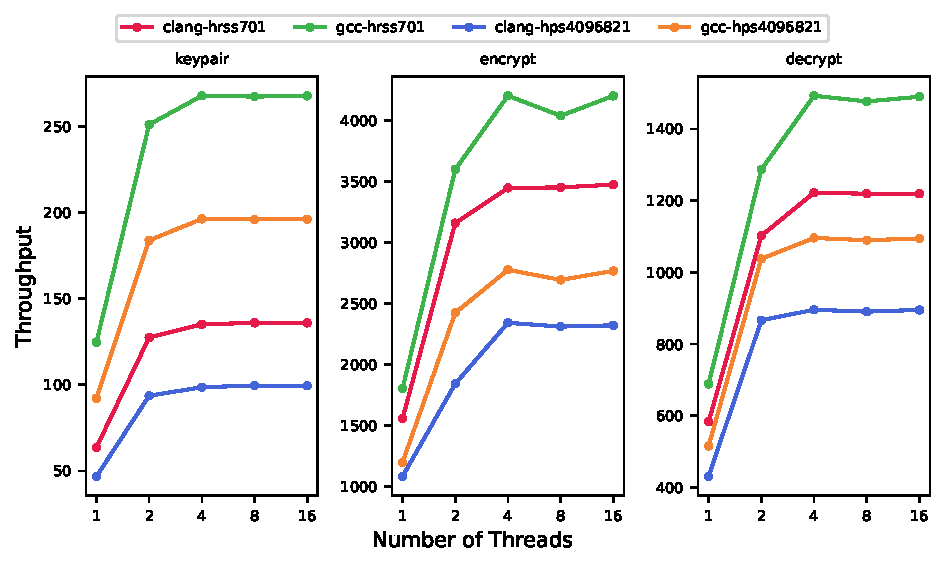
\includegraphics[scale=0.75]{chapters/results/throughput/Old Low-Range Laptop_ntru.pdf}
    \caption{Throughput of \gls{ntru} on Old Low-Range Laptop}
    \label{figure:results:throughput:ntru:old-low-range-laptop}
\end{figure}

\begin{figure}
    \centering
    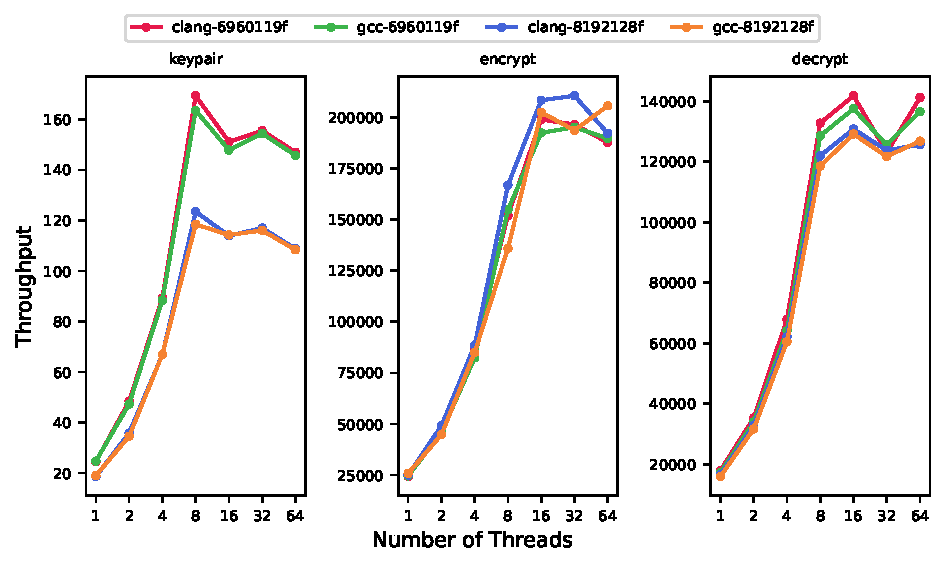
\includegraphics[scale=0.75]{chapters/results/throughput/Modern Workstation_mceliece.pdf}
    \caption{Throughput of \gls{mceliece} on Modern Workstation}
    \label{figure:results:throughput:mceliece:modern-workstation}
\end{figure}

\begin{figure}
    \centering
    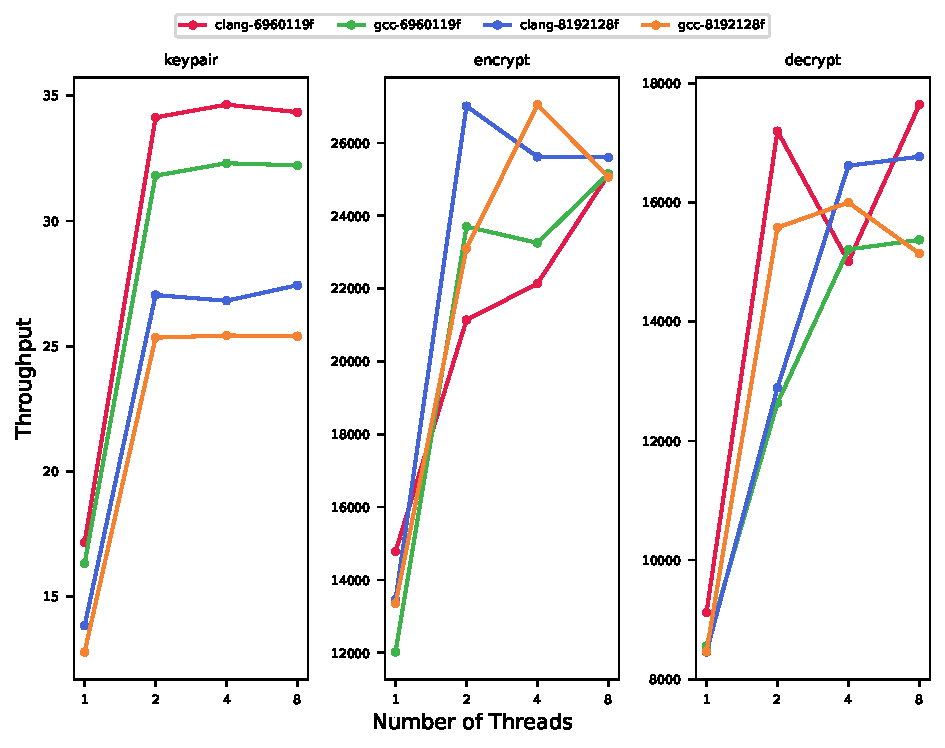
\includegraphics[scale=0.75]{chapters/results/throughput/Cloud Provider 2_mceliece.pdf}
    \caption{Throughput of \gls{mceliece} on Cloud Provider 2}
    \label{figure:results:throughput:mceliece:cloud-provider-2}
\end{figure}
\todo{Replace with the new table format?}
\begin{table}
    \centering
    \footnotesize
    \caption{Duration of \gls{mceliece} 6960119 keypair-generation for various environments}
    \label{table:results:sequential:mceliece-6960119-keypair}
    \begin{tabularx}{\linewidth}{l c c c c c c}
        \toprule
        \thead{Environment} & \thead{Compiler} & \thead{Flags} & \thead{Iterations} & \thead{Average Duration} & \thead{Speedup}\\
        \midrule
          \multirowcell{6}{Modern\\ Workstation} &                  gcc &                  ref &                   82 &           22043.51ms &                  0.0\\
          &                clang &        ref-optimized &                 2000 &             696.65ms &                 30.6\\
          &                  gcc &                 avx2 &                 2000 &             562.39ms &                 38.2\\
          &                  gcc &        ref-optimized &                 2000 &             421.15ms &                 51.3\\
          &                  gcc &       avx2-optimized &                 2000 &              72.26ms &                304.1\\
          &                clang &       avx2-optimized &                 2000 &              70.28ms &                312.7\\
          \midrule
               \multirowcell{6}{Modern\\ Laptop} &                  gcc &                  ref &                   66 &           28196.39ms &                  0.0\\
               &                clang &        ref-optimized &                 1909 &             943.48ms &                 28.9\\
               &                  gcc &                 avx2 &                 2000 &             730.56ms &                 37.6\\
               &                  gcc &        ref-optimized &                 2000 &             522.97ms &                 52.9\\
               &                  gcc &       avx2-optimized &                 2000 &              93.89ms &                299.3\\
               &                clang &       avx2-optimized &                 2000 &              91.24ms &                308.1\\
           \midrule
        \multirowcell{3}{Old Mid-Range\\ Laptop} &                  gcc &                  ref &                   54 &           35632.53ms &                  0.0\\
        &                clang &        ref-optimized &                 1130 &            1598.85ms &                 21.3\\
        &                  gcc &        ref-optimized &                 1951 &             922.80ms &                 37.6\\
        \midrule
        \multirowcell{3}{Old Low-Range\\ Laptop} &                  gcc &                  ref &                   38 &           48365.79ms &                  0.0\\
        &                clang &        ref-optimized &                  878 &            2050.63ms &                 22.6\\
        &                  gcc &        ref-optimized &                 1563 &            1154.21ms &                 40.9\\
            \midrule
            \multirowcell{6}{Cloud\\ Provider 1} &                  gcc &                  ref &                   58 &           33822.17ms &                  0.0\\
            &                  gcc &        ref-optimized &                 1715 &            1049.88ms &                 31.2\\
            &                clang &        ref-optimized &                 1816 &             993.36ms &                 33.0\\
            &                  gcc &                 avx2 &                 2000 &             865.83ms &                 38.1\\
            &                  gcc &       avx2-optimized &                 2000 &              97.95ms &                344.3\\
            &                clang &       avx2-optimized &                 2000 &              91.33ms &                369.3\\
            \midrule
            \multirowcell{6}{Cloud\\ Provider 2} &                  gcc &                  ref &                   56 &           34358.41ms &                  0.0\\
             &                clang &        ref-optimized &                 1528 &            1178.51ms &                 28.2\\
             &                  gcc &                 avx2 &                 1843 &             977.72ms &                 34.1\\
             &                  gcc &        ref-optimized &                 2000 &             698.16ms &                 48.2\\
             &                  gcc &       avx2-optimized &                 2000 &             114.33ms &                299.5\\
             &                clang &       avx2-optimized &                 2000 &             109.24ms &                313.5\\
             \midrule
         \multirowcell{3}{IBM\\ Community Cloud} &                  gcc &                  ref &                   24 &           83750.71ms &                  0.0\\
         &                clang &        ref-optimized &                 2000 &             846.66ms &                 97.9\\
         &                  gcc &        ref-optimized &                 2000 &             834.29ms &                 99.4 \\
        \bottomrule
    \end{tabularx}
\end{table}
\todo{Replace with the new table format?}
\begin{table}
    \centering
    \footnotesize
    \caption{Duration of \gls{mceliece} 6960119f keypair-generation for various environments}
    \label{table:results:sequential:mceliece-6960119f-keypair}
    \begin{tabularx}{\linewidth}{X c c c c c c}
        \toprule
        \thead{Environment} & \thead{Compiler} & \thead{Flags} & \thead{Iterations} & \thead{Average Duration} & \thead{Speedup}\\
        \midrule
          \multirowcell{6}{Modern\\ Workstation} &                  gcc &                  ref &                  277 &            6522.89ms &                  0.0\\
          &                  gcc &                 avx2 &                 2000 &             315.24ms &                 19.7\\
          &                clang &        ref-optimized &                 2000 &             230.14ms &                 27.3\\
          &                  gcc &        ref-optimized &                 2000 &             159.12ms &                 40.0\\
          &                  gcc &       avx2-optimized &                 2000 &              40.45ms &                160.2\\
          &                clang &       avx2-optimized &                 2000 &              39.93ms &                162.4\\
          \midrule
               \multirowcell{6}{Modern\\ Laptop} &                  gcc &                  ref &                  221 &            8195.28ms &                  0.0\\
               &                  gcc &                 avx2 &                 2000 &             412.25ms &                 18.9\\
               &                clang &        ref-optimized &                 2000 &             318.60ms &                 24.7\\
               &                  gcc &        ref-optimized &                 2000 &             190.31ms &                 42.1\\
               &                  gcc &       avx2-optimized &                 2000 &              50.75ms &                160.5\\
               &                clang &       avx2-optimized &                 2000 &              48.89ms &                166.6\\
               \midrule
        \multirowcell{3}{Old Mid-Range\\ Laptop} &                  gcc &                  ref &                  144 &           12574.97ms &                  0.0\\
        &                clang &        ref-optimized &                 2000 &             524.88ms &                 23.0\\
        &                  gcc &        ref-optimized &                 2000 &             328.95ms &                 37.2\\
        \midrule
         \multirowcell{3}{Old Low-Range\\ Laptop} &                  gcc &                  ref &                  113 &           16061.37ms &                  0.0\\
        &                clang &        ref-optimized &                 2000 &             665.17ms &                 23.1\\
        &                  gcc &        ref-optimized &                 2000 &             417.25ms &                 37.5\\
        \midrule
            \multirowcell{6}{Cloud\\ Provider 1} &                  gcc &                  ref &                  188 &            9639.11ms &                  0.0\\
            &                  gcc &                 avx2 &                 2000 &             479.13ms &                 19.1\\
            &                  gcc &        ref-optimized &                 2000 &             346.59ms &                 26.8\\
            &                clang &        ref-optimized &                 2000 &             346.89ms &                 26.8\\
            &                  gcc &       avx2-optimized &                 2000 &              52.91ms &                181.2\\
            &                clang &       avx2-optimized &                 2000 &              47.80ms &                200.7\\
            \midrule
           \multirowcell{6}{Cloud\\ Provider 2}  &                  gcc &                  ref &                  158 &           11485.44ms &                  0.0\\
            &                  gcc &                 avx2 &                 2000 &             556.56ms &                 19.6\\
            &                clang &        ref-optimized &                 2000 &             407.85ms &                 27.2\\
            &                  gcc &        ref-optimized &                 2000 &             253.10ms &                 44.4\\
            &                  gcc &       avx2-optimized &                 2000 &              61.08ms &                187.1\\
            &                clang &       avx2-optimized &                 2000 &              57.67ms &                198.2\\
            \midrule
          \multirowcell{3}{IBM\\ Community Cloud} &                  gcc &                  ref &                   78 &           23366.52ms &                  0.0\\
          &                  gcc &        ref-optimized &                 2000 &             332.36ms &                 69.3\\
          &                clang &        ref-optimized &                 2000 &             296.39ms &                 77.8 \\
        \bottomrule
    \end{tabularx}
\end{table}

\begin{table}[H]
    \centering
    \footnotesize
    \caption{Sequential Duration and Speedup of \gls{ntru} HPS 4096821}
    \begin{tabularx}{\linewidth}{l l c c c c c c}
        \toprule
        \thead{Environment} & \thead{Flags} & \multicolumn{3}{c}{\thead{Average Duration (ms)}} & \multicolumn{3}{c}{\thead{Speedup}}\\
        & & keypair & encrypt & decrypt & keypair & encrypt & decrypt \\
        \midrule
        \multirowcell{8}{Modern\\ Workstation}
          & \textbf{gcc} & & & & & \\
          & ref & 47.170 & 1.344 & 3.640 & 0.0 & 0.0 & 0.0\\
          & ref-optimized & 4.586 & 0.337 & 0.865 & 9.3 & 3.0 & 3.2\\
          & avx2 & 0.445 & 0.161 & 0.044 & 104.9 & 7.3 & 81.8\\
          & avx2-optimized & 0.132 & 0.058 & 0.018 & 356.5 & 22.2 & 200.7\\
          & \textbf{clang} & & & & & \\
          & ref-optimized & 7.389 & 0.303 & 0.758 & 5.4 & 3.4 & 3.8\\
          & avx2-optimized & 0.130 & 0.054 & 0.018 & 361.7 & 23.8 & 205.2\\
          \midrule
          \multirowcell{8}{Modern\\ Laptop}
          & \textbf{gcc} & & & & & \\
          & ref & 57.391 & 1.708 & 4.479 & 0.0 & 0.0 & 0.0\\
          & ref-optimized & 5.656 & 0.422 & 1.091 & 9.1 & 3.0 & 3.1\\
          & avx2 & 0.580 & 0.201 & 0.066 & 97.9 & 7.5 & 67.3\\
          & avx2-optimized & 0.168 & 0.077 & 0.029 & 341.0 & 21.2 & 152.7\\
          & \textbf{clang} & & & & & \\
          & ref-optimized & 9.136 & 0.374 & 0.970 & 5.3 & 3.6 & 3.6\\
          & avx2-optimized & 0.166 & 0.086 & 0.037 & 344.2 & 18.9 & 120.9\\
          \midrule
          \multirowcell{5}{Old\\ Mid-Range\\ Laptop}
          & \textbf{gcc} & & & & & \\
          & ref & 83.233 & 2.340 & 6.154 & 0.0 & 0.0 & 0.0\\
          & ref-optimized & 8.609 & 0.614 & 1.514 & 8.7 & 2.8 & 3.1\\
          & \textbf{clang} & & & & & \\
          & ref-optimized & 16.842 & 0.723 & 1.837 & 3.9 & 2.2 & 2.4\\
          \midrule
          \multirowcell{5}{Old\\ Low-Range\\ Laptop}
          & \textbf{gcc} & & & & & \\
          & ref & 105.791 & 2.950 & 7.703 & 0.0 & 0.0 & 0.0\\
          & ref-optimized & 10.782 & 0.767 & 1.871 & 8.8 & 2.8 & 3.1\\
          & \textbf{clang} & & & & & \\
          & ref-optimized & 21.263 & 0.901 & 2.260 & 4.0 & 2.3 & 2.4\\
          \midrule
          \multirowcell{8}{Cloud\\ Provider\\ 1}
          & \textbf{gcc} & & & & & \\
          & ref & 68.867 & 2.012 & 5.494 & 0.0 & 0.0 & 0.0\\
          & ref-optimized & 7.490 & 0.570 & 1.440 & 8.2 & 2.5 & 2.8\\
          & avx2 & 0.724 & 0.252 & 0.075 & 94.2 & 7.0 & 72.7\\
          & avx2-optimized & 0.205 & 0.102 & 0.032 & 334.9 & 18.8 & 170.2\\
          & \textbf{clang} & & & & & \\
          & ref-optimized & 11.082 & 0.442 & 1.073 & 5.2 & 3.6 & 4.1\\
          & avx2-optimized & 0.205 & 0.095 & 0.034 & 335.4 & 20.1 & 159.6\\
          \midrule
          \multirowcell{8}{Cloud\\ Provider\\ 2}
          & \textbf{gcc} & & & & & \\
          & ref & 82.797 & 2.336 & 6.265 & 0.0 & 0.0 & 0.0\\
          & ref-optimized & 7.775 & 0.565 & 1.468 & 9.6 & 3.1 & 3.3\\
          & avx2 & 0.886 & 0.308 & 0.084 & 92.4 & 6.6 & 73.5\\
          & avx2-optimized & 0.256 & 0.104 & 0.035 & 321.9 & 21.4 & 176.7\\
          & \textbf{clang} & & & & & \\
          & ref-optimized & 14.024 & 0.556 & 1.390 & 4.9 & 3.2 & 3.5\\
          & avx2-optimized & 0.277 & 0.116 & 0.049 & 298.2 & 19.2 & 127.2\\
          \midrule
          \multirowcell{5}{IBM\\ Community\\ Cloud}
          & \textbf{gcc} & & & & & \\
          & ref & 85.807 & 2.943 & 8.544 & 0.0 & 0.0 & 0.0\\
          & ref-optimized & 9.813 & 0.707 & 1.946 & 7.7 & 3.2 & 3.4\\
          & \textbf{clang} & & & & & \\
          & ref-optimized & 12.176 & 0.574 & 1.538 & 6.0 & 4.1 & 4.6\\
        \bottomrule
    \end{tabularx}
\end{table}

\begin{table}
    \centering
    \footnotesize
    \caption{Sequential duration and speedup of \gls{mceliece} 6960119}
    \begin{tabularx}{\linewidth}{l l c c c c c c}
        \toprule
        \thead{Environment} & \thead{Flags} & \multicolumn{3}{c}{\thead{Average Duration (ms)}} & \multicolumn{3}{c}{\thead{Speedup}}\\
        & & keypair & encrypt & decrypt & keypair & encrypt & decrypt \\
        \midrule
        \multirowcell{8}{Modern\\ Workstation}
          & \textbf{gcc} & & & & & \\
          & ref & 22043.511 & 8.275 & 208.689 & 0.0 & 0.0 & 0.0\\
          & ref-optimized & 421.154 & 0.179 & 57.090 & 51.3 & 45.3 & 2.7\\
          & avx2 & 562.393 & 0.083 & 0.219 & 38.2 & 98.1 & 953.7\\
          & avx2-optimized & 72.261 & 0.041 & 0.060 & 304.1 & 200.3 & 3465.6\\
          & \textbf{clang} & & & & & \\
          & ref-optimized & 696.651 & 0.574 & 52.871 & 30.6 & 13.4 & 2.9\\
          & avx2-optimized & 70.280 & 0.040 & 0.059 & 312.7 & 205.1 & 3560.2\\
          \midrule
          \multirowcell{8}{Modern\\ Laptop}
          & \textbf{gcc} & & & & & \\
          & ref & 28196.387 & 10.122 & 252.367 & 0.0 & 0.0 & 0.0\\
          & ref-optimized & 522.974 & 0.214 & 69.371 & 52.9 & 46.4 & 2.6\\
          & avx2 & 730.559 & 0.102 & 0.265 & 37.6 & 98.1 & 951.1\\
          & avx2-optimized & 93.891 & 0.047 & 0.072 & 299.3 & 213.2 & 3501.7\\
          & \textbf{clang} & & & & & \\
          & ref-optimized & 943.476 & 0.754 & 63.391 & 28.9 & 12.4 & 3.0\\
          & avx2-optimized & 91.235 & 0.049 & 0.071 & 308.1 & 205.8 & 3543.5\\
          \midrule
          \multirowcell{5}{Old\\ Mid-Range\\ Laptop}
          & \textbf{gcc} & & & & & \\
          & ref & 35632.529 & 13.801 & 403.233 & 0.0 & 0.0 & 0.0\\
          & ref-optimized & 922.804 & 0.422 & 112.504 & 37.6 & 31.7 & 2.6\\
          & \textbf{clang} & & & & & \\
          & ref-optimized & 1598.851 & 1.110 & 105.008 & 21.3 & 11.4 & 2.8\\
          \midrule
          \multirowcell{5}{Old\\ Low-Range\\ Laptop}
          & \textbf{gcc} & & & & & \\
          & ref & 48365.795 & 17.197 & 512.801 & 0.0 & 0.0 & 0.0\\
          & ref-optimized & 1154.209 & 0.482 & 142.156 & 40.9 & 34.6 & 2.6\\
          & \textbf{clang} & & & & & \\
          & ref-optimized & 2050.628 & 1.355 & 132.891 & 22.6 & 11.7 & 2.9\\
          \midrule
          \multirowcell{8}{Cloud\\ Provider\\ 1}
          & \textbf{gcc} & & & & & \\
          & ref & 33822.172 & 12.243 & 304.847 & 0.0 & 0.0 & 0.0\\
          & ref-optimized & 1049.882 & 0.538 & 97.652 & 31.2 & 21.7 & 2.1\\
          & avx2 & 865.829 & 0.140 & 0.338 & 38.1 & 86.4 & 902.3\\
          & avx2-optimized & 97.953 & 0.074 & 0.104 & 344.3 & 165.0 & 2931.6\\
          & \textbf{clang} & & & & & \\
          & ref-optimized & 993.365 & 0.803 & 77.004 & 33.0 & 14.2 & 3.0\\
          & avx2-optimized & 91.335 & 0.073 & 0.095 & 369.3 & 167.1 & 3194.5\\
          \midrule
          \multirowcell{8}{Cloud\\ Provider\\ 2}
          & \textbf{gcc} & & & & & \\
          & ref & 34358.412 & 14.286 & 361.969 & 0.0 & 0.0 & 0.0\\
          & ref-optimized & 698.161 & 0.982 & 100.213 & 48.2 & 13.6 & 2.6\\
          & avx2 & 977.725 & 0.145 & 0.405 & 34.1 & 97.6 & 892.9\\
          & avx2-optimized & 114.328 & 0.067 & 0.120 & 299.5 & 212.9 & 3011.6\\
          & \textbf{clang} & & & & & \\
          & ref-optimized & 1178.513 & 0.812 & 90.214 & 28.2 & 16.6 & 3.0\\
          & avx2-optimized & 109.242 & 0.075 & 0.107 & 313.5 & 189.0 & 3380.3\\
          \midrule
          \multirowcell{5}{IBM\\ Community\\ Cloud}
          & \textbf{gcc} & & & & & \\
          & ref & 83750.711 & 14.486 & 670.202 & 0.0 & 0.0 & 0.0\\
          & ref-optimized & 834.286 & 0.306 & 140.493 & 99.4 & 46.3 & 3.8\\
          & \textbf{clang} & & & & & \\
          & ref-optimized & 846.662 & 0.723 & 137.474 & 97.9 & 19.0 & 3.9\\
        \bottomrule
    \end{tabularx}
\end{table}

\begin{table}[H]
    \centering
    \footnotesize
    \caption{Sequential Duration and Speedup of \gls{mceliece} 6960119f}
    \begin{tabularx}{\linewidth}{l l c c c c c c}
        \toprule
        \thead{Environment} & \thead{Flags} & \multicolumn{3}{c}{\thead{Average Duration (ms)}} & \multicolumn{3}{c}{\thead{Speedup}}\\
        & & keypair & encrypt & decrypt & keypair & encrypt & decrypt \\
        \midrule
        \multirowcell{8}{Modern\\ Workstation}
          & \textbf{gcc} & & & & & \\
          & ref & 6522.888 & 8.269 & 210.444 & 0.0 & 0.0 & 0.0\\
          & ref-optimized & 159.119 & 0.176 & 57.350 & 40.0 & 45.9 & 2.7\\
          & avx2 & 315.237 & 0.086 & 0.222 & 19.7 & 94.8 & 948.0\\
          & avx2-optimized & 40.454 & 0.042 & 0.061 & 160.2 & 196.6 & 3468.8\\
          & \textbf{clang} & & & & & \\
          & ref-optimized & 230.144 & 0.572 & 52.625 & 27.3 & 13.4 & 3.0\\
          & avx2-optimized & 39.929 & 0.041 & 0.059 & 162.4 & 198.5 & 3593.3\\
          \midrule
          \multirowcell{8}{Modern\\ Laptop}
          & \textbf{gcc} & & & & & \\
          & ref & 8195.285 & 10.105 & 255.662 & 0.0 & 0.0 & 0.0\\
          & ref-optimized & 190.306 & 0.207 & 69.822 & 42.1 & 47.7 & 2.7\\
          & avx2 & 412.250 & 0.100 & 0.268 & 18.9 & 99.6 & 951.9\\
          & avx2-optimized & 50.749 & 0.047 & 0.075 & 160.5 & 214.9 & 3398.8\\
          & \textbf{clang} & & & & & \\
          & ref-optimized & 318.597 & 0.725 & 63.797 & 24.7 & 12.9 & 3.0\\
          & avx2-optimized & 48.893 & 0.049 & 0.068 & 166.6 & 207.1 & 3736.8\\
          \midrule
          \multirowcell{5}{Old\\ Mid-Range\\ Laptop}
          & \textbf{gcc} & & & & & \\
          & ref & 12574.973 & 13.928 & 403.198 & 0.0 & 0.0 & 0.0\\
          & ref-optimized & 328.954 & 0.428 & 112.997 & 37.2 & 31.5 & 2.6\\
          & \textbf{clang} & & & & & \\
          & ref-optimized & 524.883 & 1.125 & 105.375 & 23.0 & 11.4 & 2.8\\
          \midrule
          \multirowcell{5}{Old\\ Low-Range\\ Laptop}
          & \textbf{gcc} & & & & & \\
          & ref & 16061.373 & 17.181 & 512.833 & 0.0 & 0.0 & 0.0\\
          & ref-optimized & 417.250 & 0.480 & 142.189 & 37.5 & 34.8 & 2.6\\
          & \textbf{clang} & & & & & \\
          & ref-optimized & 665.167 & 1.366 & 132.851 & 23.1 & 11.6 & 2.9\\
          \midrule
          \multirowcell{8}{Cloud\\ Provider\\ 1}
          & \textbf{gcc} & & & & & \\
          & ref & 9639.109 & 12.195 & 305.319 & 0.0 & 0.0 & 0.0\\
          & ref-optimized & 346.594 & 0.553 & 98.245 & 26.8 & 21.0 & 2.1\\
          & avx2 & 479.132 & 0.142 & 0.342 & 19.1 & 84.6 & 892.3\\
          & avx2-optimized & 52.911 & 0.078 & 0.095 & 181.2 & 154.6 & 3216.3\\
          & \textbf{clang} & & & & & \\
          & ref-optimized & 346.890 & 0.789 & 76.549 & 26.8 & 14.5 & 3.0\\
          & avx2-optimized & 47.799 & 0.075 & 0.098 & 200.7 & 160.6 & 3111.3\\
          \midrule
          \multirowcell{8}{Cloud\\ Provider\\ 2}
          & \textbf{gcc} & & & & & \\
          & ref & 11485.441 & 14.316 & 359.980 & 0.0 & 0.0 & 0.0\\
          & ref-optimized & 253.096 & 0.965 & 99.923 & 44.4 & 13.8 & 2.6\\
          & avx2 & 556.559 & 0.157 & 0.382 & 19.6 & 90.5 & 942.5\\
          & avx2-optimized & 61.076 & 0.071 & 0.115 & 187.1 & 202.1 & 3123.8\\
          & \textbf{clang} & & & & & \\
          & ref-optimized & 407.846 & 0.792 & 91.166 & 27.2 & 17.1 & 2.9\\
          & avx2-optimized & 57.669 & 0.070 & 0.112 & 198.2 & 202.9 & 3213.1\\
          \midrule
          \multirowcell{5}{IBM\\ Community\\ Cloud}
          & \textbf{gcc} & & & & & \\
          & ref & 23366.524 & 14.283 & 909.385 & 0.0 & 0.0 & 0.0\\
          & ref-optimized & 332.357 & 0.301 & 140.686 & 69.3 & 46.5 & 5.5\\
          & \textbf{clang} & & & & & \\
          & ref-optimized & 296.387 & 0.716 & 137.822 & 77.8 & 18.9 & 5.6\\
        \bottomrule
    \end{tabularx}
\end{table}

\begin{table}[H]
    \centering
    \footnotesize
    \caption{Sequential Duration and Speedup of \gls{mceliece} 8192128}
    \begin{tabularx}{\linewidth}{l l c c c c c c}
        \toprule
        \thead{Environment} & \thead{Flags} & \multicolumn{3}{c}{\thead{Average Duration (ms)}} & \multicolumn{3}{c}{\thead{Speedup}}\\
        & & keypair & encrypt & decrypt & keypair & encrypt & decrypt \\
        \midrule
        \multirowcell{8}{Modern\\ Workstation}
          & \textbf{gcc} & & & & & \\
          & ref & 26945.663 & 8.193 & 263.548 & 0.0 & 0.0 & 0.0\\
          & ref-optimized & 442.630 & 0.099 & 72.095 & 59.9 & 81.7 & 2.7\\
          & avx2 & 661.355 & 0.091 & 0.233 & 39.7 & 88.9 & 1131.8\\
          & avx2-optimized & 88.744 & 0.042 & 0.066 & 302.6 & 196.2 & 4019.6\\
          & \textbf{clang} & & & & & \\
          & ref-optimized & 435.015 & 0.100 & 66.242 & 60.9 & 80.6 & 3.0\\
          & avx2-optimized & 84.821 & 0.039 & 0.064 & 316.7 & 206.4 & 4139.6\\
          \midrule
          \multirowcell{8}{Modern\\ Laptop}
          & \textbf{gcc} & & & & & \\
          & ref & 33307.574 & 10.037 & 319.317 & 0.0 & 0.0 & 0.0\\
          & ref-optimized & 560.099 & 0.109 & 87.097 & 58.5 & 90.8 & 2.7\\
          & avx2 & 862.787 & 0.106 & 0.282 & 37.6 & 94.0 & 1130.3\\
          & avx2-optimized & 113.521 & 0.048 & 0.078 & 292.4 & 208.8 & 4087.6\\
          & \textbf{clang} & & & & & \\
          & ref-optimized & 513.795 & 0.118 & 80.537 & 63.8 & 84.1 & 3.0\\
          & avx2-optimized & 113.543 & 0.047 & 0.075 & 292.3 & 214.6 & 4239.6\\
          \midrule
          \multirowcell{5}{Old\\ Mid-Range\\ Laptop}
          & \textbf{gcc} & & & & & \\
          & ref & 51647.180 & 13.356 & 508.533 & 0.0 & 0.0 & 0.0\\
          & ref-optimized & 1096.384 & 0.264 & 141.813 & 46.1 & 49.7 & 2.6\\
          & \textbf{clang} & & & & & \\
          & ref-optimized & 1017.089 & 0.254 & 133.432 & 49.8 & 51.5 & 2.8\\
          \midrule
          \multirowcell{5}{Old\\ Low-Range\\ Laptop}
          & \textbf{gcc} & & & & & \\
          & ref & 56485.791 & 16.780 & 647.400 & 0.0 & 0.0 & 0.0\\
          & ref-optimized & 1376.720 & 0.302 & 180.795 & 40.0 & 54.5 & 2.6\\
          & \textbf{clang} & & & & & \\
          & ref-optimized & 1304.079 & 0.305 & 169.034 & 42.3 & 54.1 & 2.8\\
          \midrule
          \multirowcell{8}{Cloud\\ Provider\\ 1}
          & \textbf{gcc} & & & & & \\
          & ref & 38080.543 & 12.056 & 386.312 & 0.0 & 0.0 & 0.0\\
          & ref-optimized & 707.610 & 0.183 & 122.684 & 52.8 & 65.0 & 2.1\\
          & avx2 & 1014.527 & 0.150 & 0.368 & 36.5 & 79.5 & 1049.5\\
          & avx2-optimized & 113.585 & 0.084 & 0.108 & 334.3 & 143.2 & 3590.9\\
          & \textbf{clang} & & & & & \\
          & ref-optimized & 690.924 & 0.150 & 96.631 & 54.1 & 79.5 & 3.0\\
          & avx2-optimized & 108.353 & 0.085 & 0.106 & 350.4 & 141.1 & 3640.0\\
          \midrule
          \multirowcell{8}{Cloud\\ Provider\\ 2}
          & \textbf{gcc} & & & & & \\
          & ref & 48685.711 & 14.024 & 456.320 & 0.0 & 0.0 & 0.0\\
          & ref-optimized & 805.677 & 0.876 & 126.374 & 59.4 & 15.0 & 2.6\\
          & avx2 & 1168.784 & 0.166 & 0.398 & 40.7 & 83.7 & 1144.8\\
          & avx2-optimized & 134.115 & 0.089 & 0.129 & 362.0 & 156.8 & 3548.7\\
          & \textbf{clang} & & & & & \\
          & ref-optimized & 775.170 & 0.188 & 117.180 & 61.8 & 73.8 & 2.9\\
          & avx2-optimized & 129.397 & 0.088 & 0.123 & 375.3 & 158.0 & 3699.9\\
          \midrule
          \multirowcell{5}{IBM\\ Community\\ Cloud}
          & \textbf{gcc} & & & & & \\
          & ref & 71890.504 & 16.228 & 988.576 & 0.0 & 0.0 & 0.0\\
          & ref-optimized & 868.778 & 0.155 & 177.416 & 81.7 & 103.7 & 4.6\\
          & \textbf{clang} & & & & & \\
          & ref-optimized & 981.098 & 0.182 & 173.844 & 72.3 & 88.3 & 4.7\\
        \bottomrule
    \end{tabularx}
\end{table}

\begin{table}[H]
    \centering
    \footnotesize
    \caption{Sequential Duration and Speedup of \gls{mceliece} 8192128f}
    \begin{tabularx}{\linewidth}{l l c c c c c c}
        \toprule
        \thead{Environment} & \thead{Flags} & \multicolumn{3}{c}{\thead{Average Duration (ms)}} & \multicolumn{3}{c}{\thead{Speedup}}\\
        & & keypair & encrypt & decrypt & keypair & encrypt & decrypt \\
        \midrule
        \multirowcell{8}{Modern\\ Workstation}
          & \textbf{gcc} & & & & & \\
          & ref & 8588.338 & 8.196 & 264.055 & 0.0 & 0.0 & 0.0\\
          & ref-optimized & 163.637 & 0.096 & 72.070 & 51.5 & 84.6 & 2.7\\
          & avx2 & 391.461 & 0.090 & 0.234 & 20.9 & 90.5 & 1129.1\\
          & avx2-optimized & 53.787 & 0.043 & 0.066 & 158.7 & 188.1 & 4021.2\\
          & \textbf{clang} & & & & & \\
          & ref-optimized & 155.167 & 0.097 & 66.796 & 54.3 & 83.2 & 3.0\\
          & avx2-optimized & 51.880 & 0.042 & 0.064 & 164.5 & 196.5 & 4154.1\\
          \midrule
          \multirowcell{8}{Modern\\ Laptop}
          & \textbf{gcc} & & & & & \\
          & ref & 10736.023 & 10.024 & 318.262 & 0.0 & 0.0 & 0.0\\
          & ref-optimized & 208.830 & 0.114 & 87.173 & 50.4 & 86.6 & 2.7\\
          & avx2 & 513.274 & 0.104 & 0.281 & 19.9 & 94.9 & 1130.2\\
          & avx2-optimized & 65.011 & 0.046 & 0.078 & 164.1 & 217.6 & 4084.5\\
          & \textbf{clang} & & & & & \\
          & ref-optimized & 189.626 & 0.115 & 79.783 & 55.6 & 86.2 & 3.0\\
          & avx2-optimized & 62.089 & 0.048 & 0.079 & 171.9 & 205.9 & 4045.6\\
          \midrule
          \multirowcell{5}{Old\\ Mid-Range\\ Laptop}
          & \textbf{gcc} & & & & & \\
          & ref & 16400.446 & 13.393 & 508.357 & 0.0 & 0.0 & 0.0\\
          & ref-optimized & 382.143 & 0.253 & 141.827 & 41.9 & 52.0 & 2.6\\
          & \textbf{clang} & & & & & \\
          & ref-optimized & 365.884 & 0.259 & 133.069 & 43.8 & 50.7 & 2.8\\
          \midrule
          \multirowcell{5}{Old\\ Low-Range\\ Laptop}
          & \textbf{gcc} & & & & & \\
          & ref & 20971.226 & 16.782 & 647.595 & 0.0 & 0.0 & 0.0\\
          & ref-optimized & 487.037 & 0.305 & 180.696 & 42.1 & 54.0 & 2.6\\
          & \textbf{clang} & & & & & \\
          & ref-optimized & 461.702 & 0.303 & 168.017 & 44.4 & 54.3 & 2.9\\
          \midrule
          \multirowcell{8}{Cloud\\ Provider\\ 1}
          & \textbf{gcc} & & & & & \\
          & ref & 12602.279 & 12.301 & 386.733 & 0.0 & 0.0 & 0.0\\
          & ref-optimized & 260.829 & 0.170 & 123.386 & 47.3 & 71.3 & 2.1\\
          & avx2 & 590.632 & 0.160 & 0.356 & 20.3 & 75.9 & 1084.4\\
          & avx2-optimized & 66.302 & 0.087 & 0.105 & 189.1 & 140.6 & 3673.4\\
          & \textbf{clang} & & & & & \\
          & ref-optimized & 252.171 & 0.149 & 96.540 & 49.0 & 81.8 & 3.0\\
          & avx2-optimized & 60.345 & 0.082 & 0.099 & 207.8 & 148.1 & 3897.5\\
          \midrule
          \multirowcell{8}{Cloud\\ Provider\\ 2}
          & \textbf{gcc} & & & & & \\
          & ref & 15300.268 & 14.009 & 455.207 & 0.0 & 0.0 & 0.0\\
          & ref-optimized & 290.035 & 0.935 & 126.265 & 51.8 & 14.0 & 2.6\\
          & avx2 & 684.134 & 0.166 & 0.391 & 21.4 & 83.5 & 1163.1\\
          & avx2-optimized & 77.073 & 0.107 & 0.134 & 197.5 & 130.0 & 3396.1\\
          & \textbf{clang} & & & & & \\
          & ref-optimized & 281.187 & 0.196 & 113.827 & 53.4 & 70.4 & 3.0\\
          & avx2-optimized & 73.824 & 0.091 & 0.125 & 206.3 & 153.3 & 3630.5\\
          \midrule
          \multirowcell{5}{IBM\\ Community\\ Cloud}
          & \textbf{gcc} & & & & & \\
          & ref & 27835.442 & 17.092 & 834.731 & 0.0 & 0.0 & 0.0\\
          & ref-optimized & 360.210 & 0.157 & 177.614 & 76.3 & 108.0 & 3.7\\
          & \textbf{clang} & & & & & \\
          & ref-optimized & 350.169 & 0.181 & 173.950 & 78.5 & 93.5 & 3.8\\
        \bottomrule
    \end{tabularx}
\end{table}

\begin{figure}
    \centering
    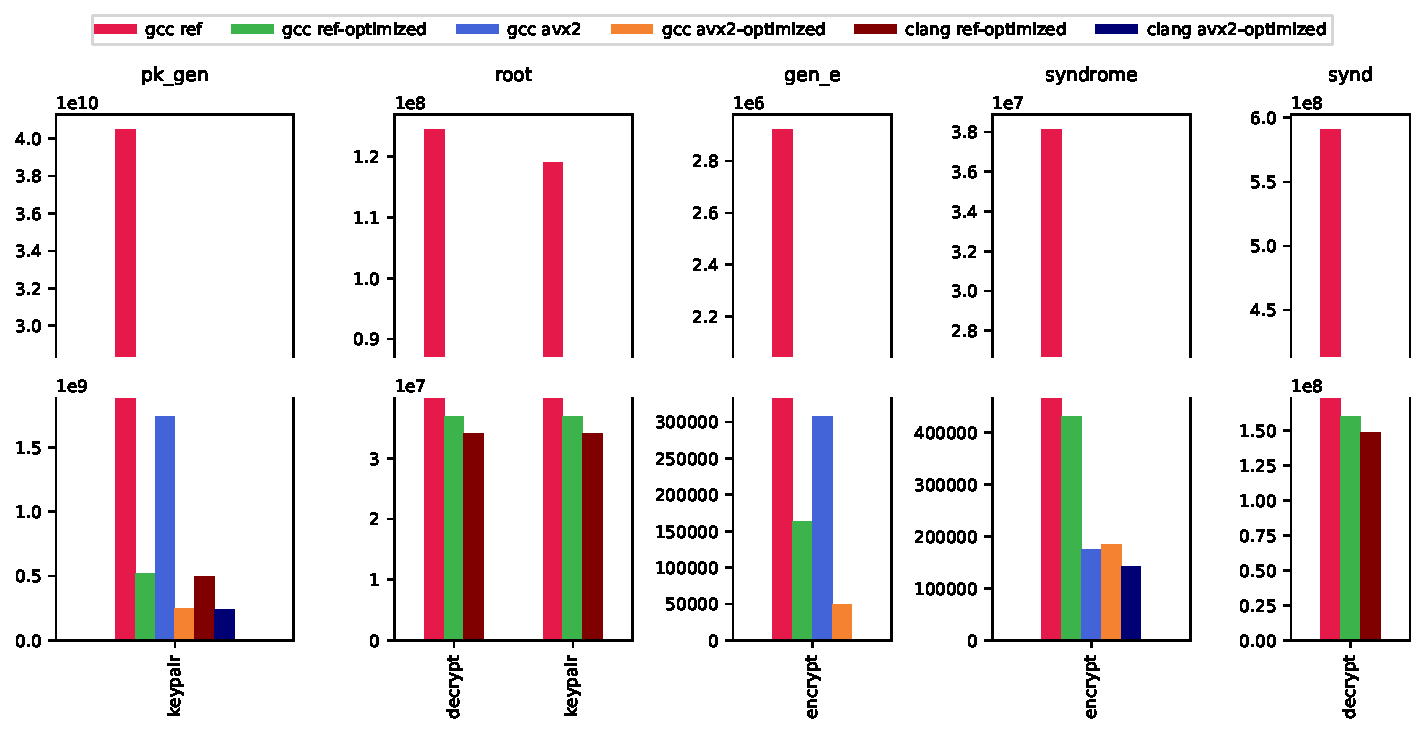
\includegraphics[width=\textwidth]{chapters/results/micro/mceliece_8192128f_Modern Workstation_cpu-cycles.pdf}
    \caption{CPU cycles consumed for \gls{mceliece} 8192128f on Modern Workstation}
    \label{figure:results:micro:mceliece-8192128f-modern-workstation}
\end{figure}

\begin{figure}
    \centering
    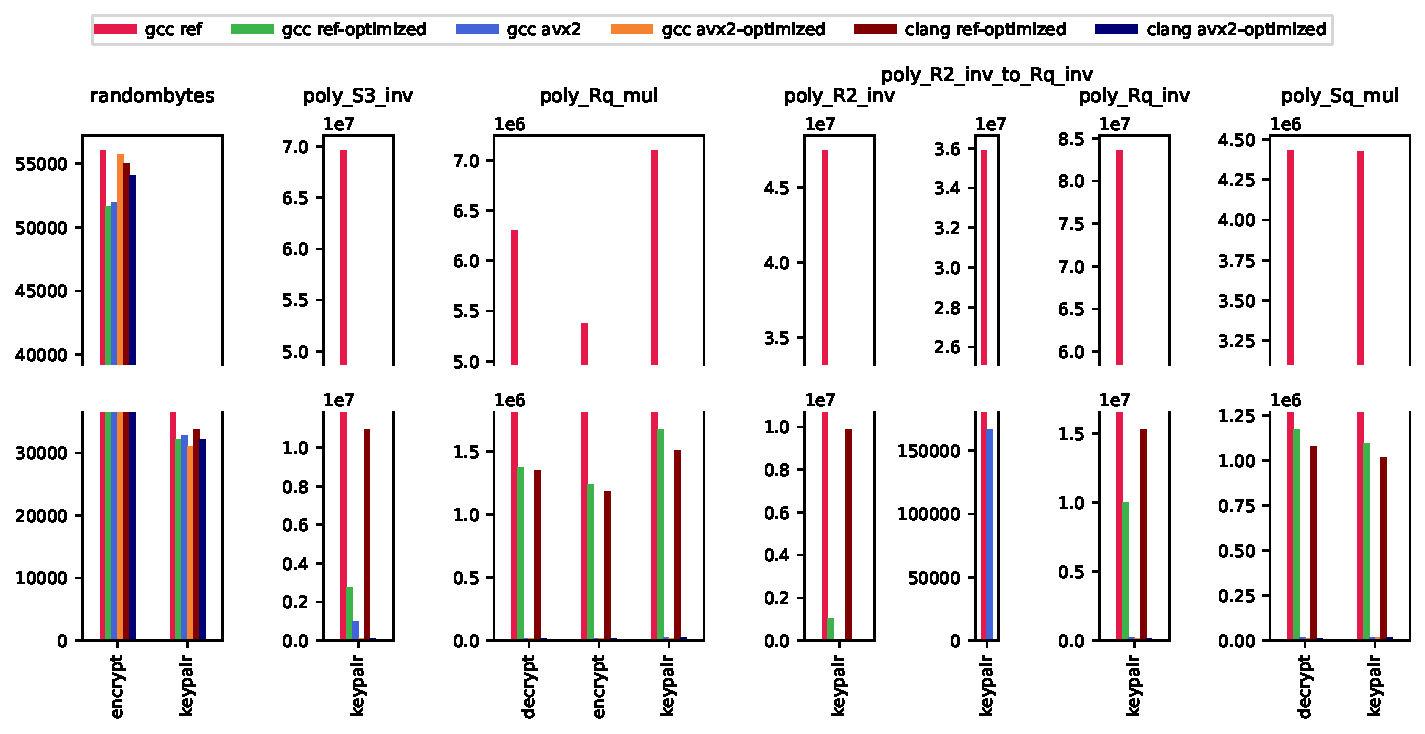
\includegraphics[width=\textwidth]{chapters/results/micro/ntru_hrss701_Modern Laptop_cpu-cycles.pdf}
    \caption{CPU cycles consumed for \gls{ntru} HRSS 701 on Modern Laptop}
    \label{figure:results:micro:ntru-hrss701-modern-laptop}
\end{figure}

% DO NOT CHANGE BELOW
% This part makes sure that the last page is even with BTH-logo.
% -------------------
\cleardoublepage
\thispagestyle{empty}
\vspace*{\fill}
\clearpage{\thispagestyle{empty}}
\changepage{3cm}{1cm}{-0.5cm}{-0.5cm}{}{-1.5cm}{}{}{}
\vspace*{\fill}
\center

{\bthcsnotextlogo{3cm}}
\\
\noindent\makebox[\linewidth]{\rule{\textwidth}{1pt}} 
Faculty of \faculty, Blekinge Institute of Technology, 371 79 Karlskrona, Sweden
% -------------------

\end{document}
